\documentclass[11pt,b5paper,twoside]{book}

%\usepackage{algorithm}  
%\usepackage{algorithmic}  
\usepackage{wallpaper} %使用wallpaper宏包

\usepackage[final]{pdfpages} %插入整页pdf
\usepackage[T1]{fontenc}
\usepackage{CJK}
\usepackage[utf8]{inputenc}
\usepackage{amsmath}
\usepackage{amsfonts}
\usepackage{amssymb}
\usepackage{subfigure}
\usepackage{graphicx}
\usepackage{grffile}
\usepackage{epstopdf}%支持eps格式图
\usepackage[centerlast]{caption}
\counterwithin{figure}{section} %图按照章节编号
\counterwithin{equation}{section} %公式按照章节编号
\counterwithin{table}{section} %表按照章节编号
%\usepackage{fourier}
\usepackage[left=2cm,right=2cm,top=2cm,bottom=2cm]{geometry}

\usepackage[export]{adjustbox}
\graphicspath{ {./images/} }

%设置缩进
\usepackage{indentfirst} 
\setlength{\parindent}{2em}

%设置行距
\linespread{1.4}

%设置章节显示
\usepackage[center]{titlesec}
%\titleformat{\chapter}
\definecolor{gray75}{gray}{0.75}
\newcommand{\hsp}{\hspace{20pt}}
\titleformat{\chapter}{\Huge\bfseries}{第\,\thechapter\,章\hsp\textcolor{gray75}{|}\hsp}{0pt}{\Huge\bfseries}

\makeatletter %使\subsection中的内容左对齐
\renewcommand{\subsection}{\@startsection{subsection}{2}{0mm}
  {-\baselineskip}{0.5\baselineskip}{\bf\leftline}}


% 更改目录的章显示
\usepackage{titletoc}
\titlecontents{chapter}[0pt]{\addvspace{1.5pt}\filright\bf}%
               {\contentspush{第\,\thecontentslabel\,章\quad}}%
               {}{\titlerule*[8pt]{.}\contentspage}

% 更改页眉页脚为第几章形式
%\usepackage{fancyhdr}%导入fancyhdr包
%\pagestyle{fancy}
%\fancyhead{} % 初始化页眉
%\renewcommand{\chaptermark}[1]{\markboth{#1}{}}
\renewcommand{\chaptermark}[1]{\markboth{\begin{CJK}{UTF8}{gkai}第\,\thechapter\,章\, #1\end{CJK}}{}}
\renewcommand{\sectionmark}[1]{\markright{\thesection\, #1}}


%\fancyhead[LE]{\textsl{\rightmark}}
%\fancyhead[RO]{\textsl{\leftmark}}
%\renewcommand{\sectionmark}[1]{\markright{\thesection\,节\, #1}}
%\renewcommand{\chaptermark}[1]{\markright{第\,\thechapter\,章\, #1}{}}

%c++代码显示环境
\usepackage{listings}
\lstset{language=C++}

%算法伪代码环境
\usepackage[ruled,vlined]{algorithm2e}
%\usepackage[linesnumbered,lined,boxed,commentsnumbered]{algorithm2e}
%\usepackage{algorithm}
%\usepackage{algorithmic}

%更改目录
\renewcommand{\contentsname}{目录}

% 更改算法显示为中文
\renewcommand{\algorithmcfname}{算法}

%更改图表的显示
\renewcommand{\figurename}{图}
\renewcommand{\tablename}{表}

\begin{document}
\begin{CJK}{UTF8}{gkai}

 
\begin{titlepage}
  \vspace*{1cm}
	\begin{center}
		{\Huge \textbf{图形瑰宝}\par}
		{\large \textbf{第三册}\par}
		%{\Huge\raggedright 图形瑰宝\par}
  		%\noindent\hrulefill\par
  		\vspace*{1cm}
  		{\large\raggedleft david kirk  著\par}
  		{\large\raggedleft 郭飞  译\par}
  		
  		\vfill
  		{\Large 2022年\par}
  		%{\Large\raggedleft Institute\par}
	\end{center}
\end{titlepage} 
\end{CJK}
%\begin{titlingpage}
%\maketitle
%\end{titlingpage}
%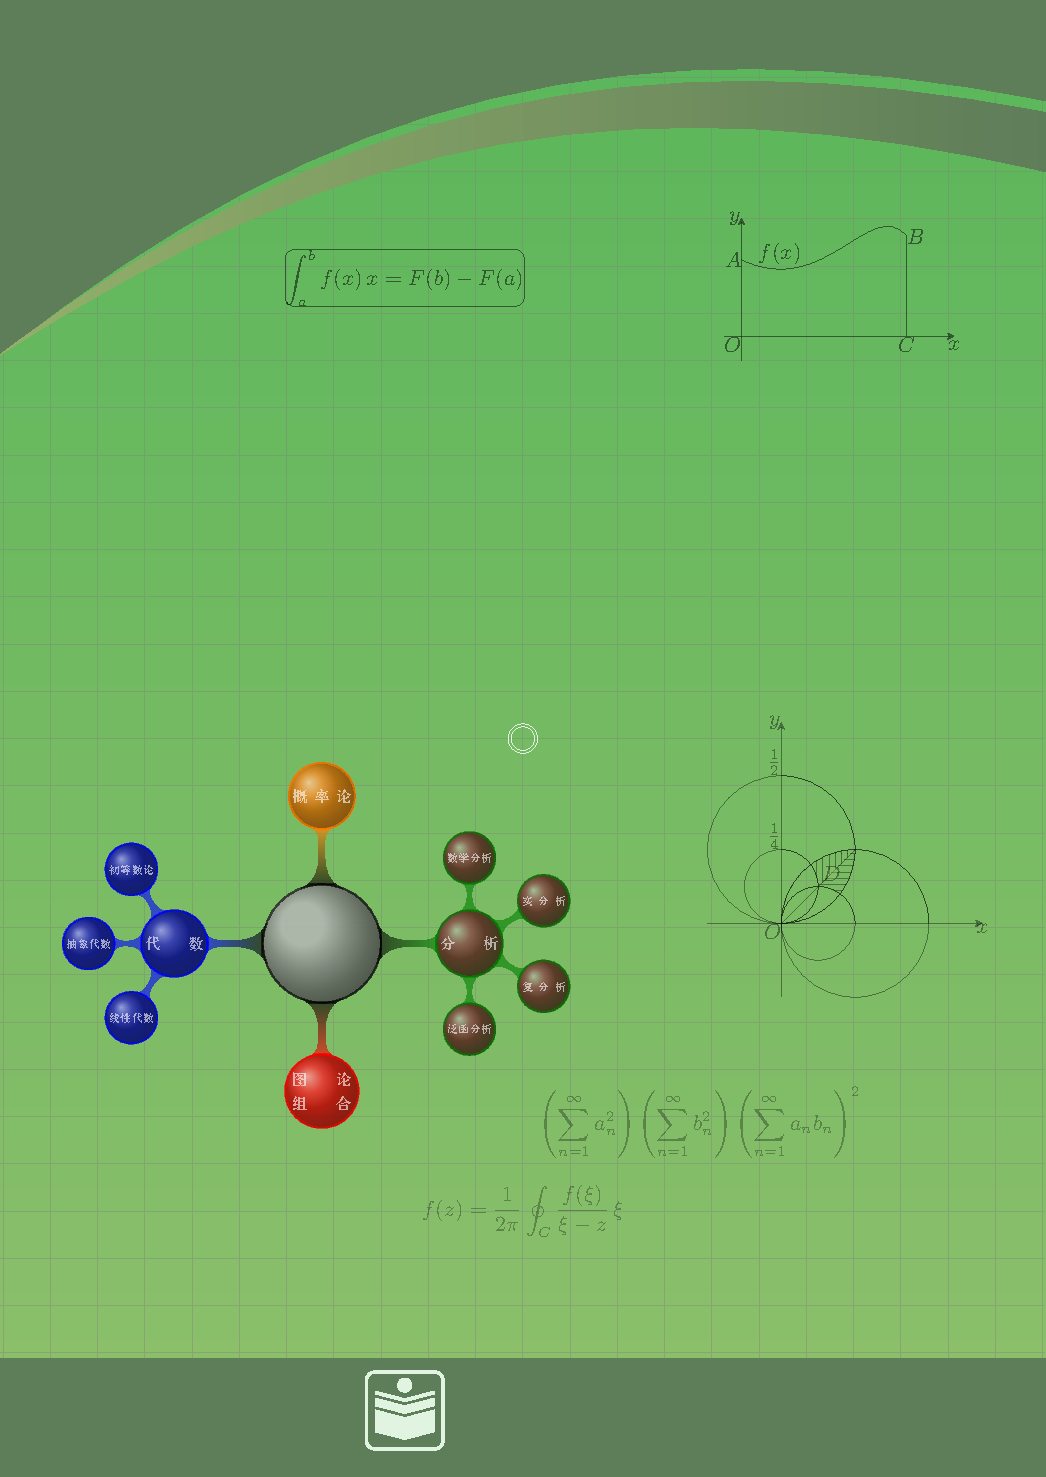
\includepdf{booktest (another copy).pdf}

%\newpage

%\maketitle

%\ThisCenterWallPaper{0.5}{./fig/cover.png}


\begin{CJK}{UTF8}{gbsn}
\tableofcontents

\newpage
\begin{CJK}{UTF8}{gkai}
\chapter{图像处理}
\end{CJK}


\begin{CJK}{UTF8}{gbsn}


本章中的所有算法都涉及对图像或像素的二维数组执行的操作。通常,图形程序员可能想要更改图像的大小、颜色或其他功能。前三个算法描述了在各种环境下拉伸或缩放图像的技术。第一条强调速度,而第二条强调质量。第四个算法描述了一种使用简化的颜色集显示全彩色图像的方法。


在某些情况下,将多个图像的特征组合起来是很有用的。第七个算法将我们现在熟悉的图像组合代数应用于黑白位图或1位图像。第八个算法讨论了如何有选择地模糊两幅图像,同时结合它们,以模拟相机的光圈景深效果。


有时,期望的结果不是另一个图像,而是图像中某些特征的另一种表示。第五、第六和第九算法描述了从图像中提取区域边界信息的技术。


\newpage
\section{位图快速拉伸}
\begin{center}
\small{
Tomas M\"oller\\
Lund Institute of Technology 
Hoganas, Sweden}
\end{center}

\subsection*{介绍}

这里提出了一个整数算法,用于将位图的任意水平线或垂直线拉伸到任何其他任意直线上。该算法可用于要求接近实时性或实时性的绘图和绘图程序。应用程序区域的例子包括扩大和缩小位图的矩形区域,以及将矩形区域包装到圆形区域上。
\subsection*{算法}
程序本身非常简单,大多数计算机图形程序员可能都熟悉它所基于的Bresenham划线算法(1965)。事实上,它可以基于任何画线算法;然而,Bresenham被选中,因为它是基于整数的,并且在计算机图形社区中非常普遍。对于那些不熟悉Bresenham算法的人来说,伪代码用于在第一个八边形中绘制线段。

\IncMargin{1em}
\begin{algorithm} 
\SetKwData{Left}{left}
\SetKwData{This}{this}
\SetKwData{Up}{up} 
\SetKwFunction{Union}{Union}
\SetKwFunction{WritePixel}{WritePixel}
\SetKwFunction{FindCompress}{FindCompress} 
\SetKwInOut{Input}{input}
\SetKwInOut{Output}{output}

\SetKwData{EdgeSet}{EdgeSet}
\SetKwData{Point}{point}
	
	\Input{由点(x1,y1)和点(x2,y2)构成的线段} 
	\Output{将线段绘制到位图上}
	 \BlankLine 
	 \BlankLine
	 
	 
	 
	 \tcp{从(x1, y1)到(x2, y2)在第一个八边形内画一条线;
所有变量都是整数}
	dx $\leftarrow$ x2 - x1\\
	dy $\leftarrow$ y2 - y1\\
	e $\leftarrow$ 2 * dy - dx\\
	\For{i$\leftarrow$ 1,i$\leqslant$ dx, i$\leftarrow$ i+1}{
		\WritePixel(x1,y1)	\tcp{在图上显示(x1,y1)}
		\While{e$\geqslant$ 0}{
			y1 $\leftarrow$ y1 + 1\\
			e $\leftarrow$ e - 2 * dx\\
		}
		x1 $\leftarrow$ x1 + 1\\
		e $\leftarrow$ e + 2 * dy
	}
	 
	 
	 
 	 	  \caption{Line(x1,y1,x2,y2)}
 	 	  \label{algo:Line} 
 	 \end{algorithm}
\DecMargin{1em} 

上面的伪代码也适用于第二个八分位数,但是在这种情况下,行不会是连续的,因为x1总是递增1。这非常适合算法。


让我们回到拉伸算法的解释上。x1和y1不能被解释为二维直线上的一对坐标,它们必须被解释为一维坐标。dx必须解释为目标线的长度,dy是源线的长度。使用这些解释,x1是目标线上的坐标,y1是源线上的坐标。对于目标线上的每个像素,从源线上选择一个像素。这些像素以统一的方式选择。参见图\ref{fig:drawline}。
\begin{figure}[htbp]%[htbp]
  \centering
  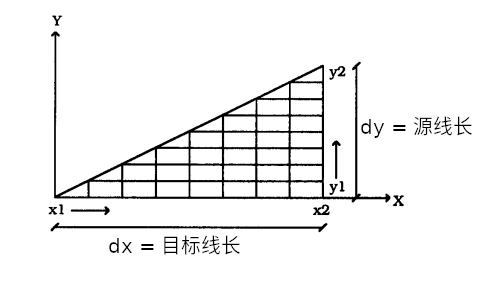
\includegraphics[totalheight=2in]{./fig/1.png}
  \caption{源线与目标线} 
  \label{fig:drawline}
\end{figure}

如果$dx$大于$dy$,那么目标线比源线长。因此,在绘制到目的线上时,源线将被放大。另一方面,如果$dy$大于$dx$,源线就会减小。如果$dx = dy$,算法会得到与源相同的直线。下面是伪代码中完整的stretcher算法,重写后能够处理$x2 < x1$和$y2 < y1$的行。

\IncMargin{1em}
\begin{algorithm} 
\SetKwData{Left}{left}
\SetKwData{This}{this}
\SetKwData{Up}{up} 
\SetKwFunction{Union}{Union}
\SetKwFunction{WritePixel}{WritePixel}
\SetKwFunction{Abs}{abs}
\SetKwFunction{Sign}{sign}
\SetKwFunction{ReadPixel}{ReadPixel}
\SetKwFunction{SetColor}{SetColor}
\SetKwFunction{FindCompress}{FindCompress} 
\SetKwInOut{Input}{input}
\SetKwInOut{Output}{output}

\SetKwData{EdgeSet}{EdgeSet}
\SetKwData{Point}{point}
	
	\Input{} 
	\Output{}
	 \BlankLine 
	 \BlankLine
	 
	 
	 
	 \tcp{从(x1, y1)到(x2, y2)在第一个八边形内画一条线;
所有变量都是整数}
	\tcp{将源线(y1 ~ y2)延伸到目标线(x1 ~ x2)。}
	\tcp{源线和目标线都是水平的}
	\tcp{yr =从其中读取像素的水平线}
	\tcp{yw =要写入像素的水平线}
	\tcp{ReadPixel(x, y)返回像素(x, y)处的颜色}
	\tcp{WritePixel(x, y) 用当前颜色写入(x, y)处的像素}
	\tcp{SetColor(Color) 设置当前写入的颜色为Color}
	dx $\leftarrow$ \Abs(x2 - x1)\\
	dy $\leftarrow$ \Abs(y2 - y1)\\
	sx $\leftarrow$ \Sign(x2 - x1)\\
	sy $\leftarrow$ \Sign(y2 - y1)\\
	e $\leftarrow$ 2 * dy - dx\\
	dx2 $\leftarrow$ 2 * dx\\
	dy $\leftarrow$ 2 * dy\\
	\For{i$\leftarrow$ 1,i$\leqslant$ dx, i$\leftarrow$ i+1}{
		color $\leftarrow$ \ReadPixel(x, y)\\
		\SetColor(Color)\\
		WritePixel(x1, yw)
		
		\While{e$\geqslant$ 0}{
			y1 $\leftarrow$ y1 + sy\\
			e $\leftarrow$ e - dx2\\
		}
		x1 $\leftarrow$ x1 + 1\\
		e $\leftarrow$ e + 2 * dy
	}
	 
	 
	 
 	 	  \caption{Stretch(x1, y1, x2, y2, yr, yw)}
 	 	  \label{algo:Stretch} 
 	 \end{algorithm}
\DecMargin{1em} 

如果$x$等于0,那么符号函数不需要返回0,因为$dx$或$dy$都等于0,这意味着一条长度为1的直线。由于该算法只使用整数运算,而不使用乘法或除法,因此非常高效和快速。


这个小程序的另一个有趣之处是,它可以用来生成几种不同形状的位图。下面列出了一些可以用来渲染的东西。
\subsection*{一些项目使用位图扩展器}
\begin{itemize}
	\item 包裹在圆形或椭圆形区域上的矩形图片。关于绕圈,请参阅附录中的源代码。
	\item 放大和缩小位图的矩形部分。参见附录中的源代码。
	\item 将位图的矩形部分绕平行梯形包绕。例如,一个绕x或y轴旋转,然后进行透视转换的矩形可以用作目标形状。
\end{itemize}


\subsection*{进一步的工作}
为了改进算法,也许可以添加一个抗锯齿例程.\\
See also G1, 147; G1, 166; G3, A.2.




\newpage
\section{一般的滤波图像缩放}
\begin{center}
\small{
Dale Schumacher\\
St. Paul, Minnesota}
\end{center}


栅格图像可以看作是连续二维函数$f(x, y)$的样本的矩形网格。这些样本被假定为连续函数在给定样本点的精确值。理想的光栅图像缩放程序包括重建原始的连续函数,然后以不同的速率重新采样该函数(Pratt, 1991;Foley $ et al$., 1990 )。采样率越高(采样越靠近),采样就越多,图像也就越大。采样率越低(采样间隔越远)产生的样本越少,因此图像越小。幸运的是,我们不需要真正地重建整个连续函数,而只是确定重建函数在与新样本对应的点上的值,这是一个更容易的任务(Smith, 1981)。仔细选择过滤器,这个重采样过程可以分两步进行,首先水平地拉伸或缩小图像,然后垂直地拉伸或缩小(反之亦然),可能有不同的比例因子。双通道方法的运行时成本$O$(image\_width*image\_height* (filter\_width + filter\_height)比简单的二维过滤$O$(image\_width*image\_height*filter\_width*filter\_height)要低得多。

\begin{figure}[htbp]%[htbp]
  \centering
  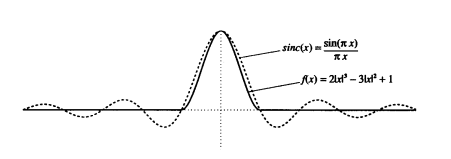
\includegraphics[totalheight=1.7in]{./fig/1.2.1.png}
  \caption{$sinc$示例} 
  \label{fig:sinc}
\end{figure}

放大图像的过程有很多名字,包括放大、拉伸、缩放、插值和上采样。我将把这个过程称为放大。缩小图像的过程也有很多名字,包括缩小、缩小、按比例缩小、抽取和下采样。我将把这个过程称为简化。这些过程将在一维而不是二维中进行解释,因为缩放是在每个轴上独立进行的。

在放大过程中,我们通过应用滤波函数来确定每个源像素对每个目标像素的贡献。采样理论表明,$sinc$函数$f(x) = \sin(πx)/πx$是理想的重构函数;然而,我们有一个有限的样本集,并且需要一个具有有限支持的过滤器(即过滤器非零的区域)。我在这个例子中使用的过滤器是一个三次函数,$f(x) = 2|x| 3 - 3|x| 2 +1$,从- 1到+1,当单独应用时,它覆盖了每个样本的单位体积。图1比较了这些过滤函数。重采样滤波器的设计是一个没完没了的争论的来源,超出了这个宝石的范围,但在许多其他作品中讨论(Pratt, 1991; Turkowski, 1990; Mitchell, 1988; Smith, 1982; Oppenheim and Schafer, 1975; Rabiner and Gold, 1975).。为了应用滤镜,我们将滤镜函数的副本放在每个源像素的中心,并缩放到该像素的高度。对于每个目标像素,我们计算源图像中相应的位置。我们将这一点上加权滤波函数的值相加,以确定目标像素的值。图\ref{fig:sinc2}说明了这个过程。

\begin{figure}[htbp]%[htbp]
  \centering
  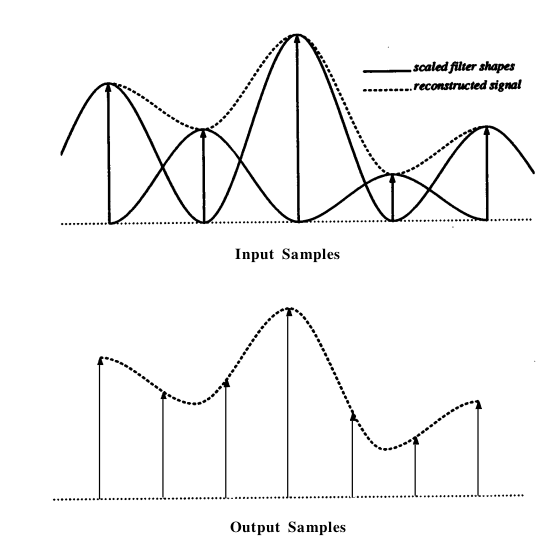
\includegraphics[totalheight=4in]{./fig/1.2.2.png}
  \caption{滤波示例} 
  \label{fig:sinc2}
\end{figure}

在缩小过程中,过程是相似的,但不完全相同,因为我们必须考虑频率混叠。采样理论将奈奎斯特频率定义为能够正确捕获连续源信号中所有频率成分的采样率。奈奎斯特频率是源信号中最高频率分量频率的两倍。任何频率成分高于采样率的一半将被不正确地采样,并将被混叠到一个更低的频率。

因此,重构信号将只包含采样率的一半或更少的频率成分。在放大过程中,我们拉伸重构信号,降低其分量频率。然而,在缩小过程中,我们正在缩小重构信号,提高其分量频率,并可能超过我们新的采样率的奈奎斯特频率。为了创建合适的样本,我们必须消除重采样奈奎斯特频率以上的所有频率成分。这可以通过图像缩小因子拉伸滤波函数来实现。此外,由于每个源像素处的滤波器更宽,和将按比例更大,并应除以相同的因子进行补偿。图\ref{fig:sinc3}说明了这个过程。

\begin{figure}[htbp]%[htbp]
  \centering
  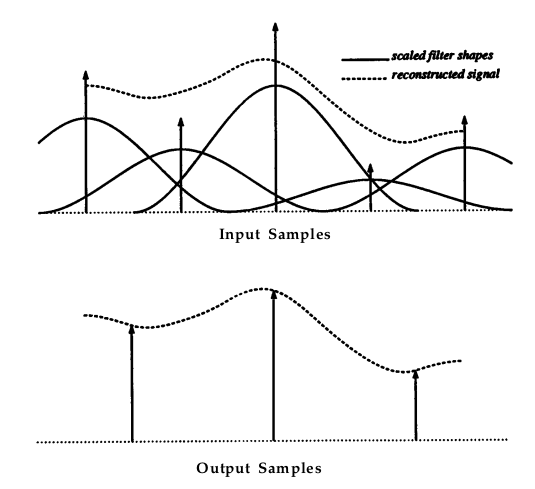
\includegraphics[totalheight=4in]{./fig/1.2.3.png}
  \caption{滤波示例} 
  \label{fig:sinc3}
\end{figure}

到目前为止,我们只考虑了一维情况。我们将其扩展到典型的光栅图像的二维情况,首先水平缩放,然后垂直缩放。这里将不再演示缩放最小目标轴的进一步优化。滤波操作会导致大量的计算,所以我们尽可能多地预先计算。每个行(或列)的缩放过程是相同的。过滤器的位置和面积是固定的;这样,我们就可以预先计算出每个目标像素的贡献者和相应的滤波器权值。计算目标像素贡献者的伪代码如\ref{algo:calculate_contributions}。

\IncMargin{1em}
\begin{algorithm} 
\SetKwData{Left}{left}
\SetKwData{This}{this}
\SetKwData{Up}{up} 
\SetKwFunction{Union}{Union}
\SetKwFunction{WritePixel}{WritePixel}
\SetKwFunction{Abs}{abs}
\SetKwFunction{Floor}{floor}
\SetKwFunction{Ceiling}{ceiling}
\SetKwFunction{Sign}{sign}
\SetKwFunction{ReadPixel}{ReadPixel}
\SetKwFunction{SetColor}{SetColor}
\SetKwFunction{FindCompress}{FindCompress} 
\SetKwFunction{Filter}{filter}
\SetKwFunction{AddContributor}{add\_contributor}

\SetKwInOut{Input}{input}
\SetKwInOut{Output}{output}

\SetKwData{EdgeSet}{EdgeSet}
\SetKwData{Point}{point}
	
	\Input{} 
	\Output{}
	 \BlankLine 
	 \BlankLine
	 
	 
	 
	 %\tcp{从(x1, y1)到(x2, y2)在第一个八边形内画一条线;所有变量都是整数}
	
	scale $\leftarrow$ dst\_size/src\_size;\\
	center $\leftarrow$ destination/scale;\\
	\If{scale < 1.0}{
		width $\leftarrow$ filter\_width/scale;\\
		fscale $\leftarrow$ 1.0/scale;\\
	}
	\lElse{
		width $\leftarrow$ filter\_width;\\
		fscale $\leftarrow$ 1.0;\\	
	}
	left $\leftarrow$ \Floor(center - width);\\
	right $\leftarrow$ \Ceiling(center + width);\\
	\For{source $\leftarrow$ left,source $\leftarrow$ source + 1, source $\leqslant$ right}{
		weight ← \Filter((center – source)/fscale)/fscale;
		\AddContributor(destination, source, weight);
	}
	 
	 
	 
 	 	  \caption{calculate\_contributions(destination)}
 	 	  \label{algo:calculate_contributions} 
 	 \end{algorithm}
\DecMargin{1em} 

在计算出贡献之后,目标图像的所有行(或列)都可以使用相同的预计算的过滤器值进行处理。下面的伪代码\ref{algo:scale_row}显示了这些值用于扩展单个目标行的应用程序。

\IncMargin{1em}
\begin{algorithm} 
\SetKwData{Left}{left}
\SetKwData{This}{this}
\SetKwData{Up}{up} 
\SetKwFunction{Union}{Union}
\SetKwFunction{WritePixel}{WritePixel}
\SetKwFunction{Abs}{abs}
\SetKwFunction{Floor}{floor}
\SetKwFunction{Ceiling}{ceiling}
\SetKwFunction{Sign}{sign}
\SetKwFunction{ReadPixel}{ReadPixel}
\SetKwFunction{SetColor}{SetColor}
\SetKwFunction{FindCompress}{FindCompress} 
\SetKwFunction{Filter}{filter}
\SetKwFunction{AddContributor}{add\_contributor}

\SetKwInOut{Input}{输入}
\SetKwInOut{Output}{输出}

\SetKwData{EdgeSet}{EdgeSet}
\SetKwData{Point}{point}
	
	\Input{} 
	\Output{}
	 \BlankLine 
	 \BlankLine
	 
	 
	 
	 %\tcp{从(x1, y1)到(x2, y2)在第一个八边形内画一条线;所有变量都是整数}
	
	\For{ i ← 0, i ← i + 1, i < dst\_size }{
		v ← 0;\\
		\For{ j ← 0, j ← j + 1, j < contributors[i] }{
			s ← contributor[i][j];\\
			w ← weight\_value[i][j];\\
			v ← v + (source\_row[s]*w);\\
		}
		destination\_row[i] ← v;\\
	}
	
 	 	  \caption{scale\_row(destination\_row, source\_row)}
 	 	  \label{algo:scale_row} 
 	 \end{algorithm}
\DecMargin{1em} 


\begin{figure}[htbp]%[htbp]
  \centering
  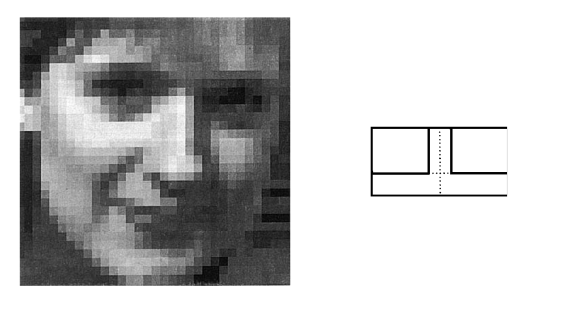
\includegraphics[totalheight=2in]{./fig/1.2.4.png}
  \caption{滤波示例} 
  \label{fig:sinc4}
\end{figure}

\begin{figure}[htbp]%[htbp]
  \centering
  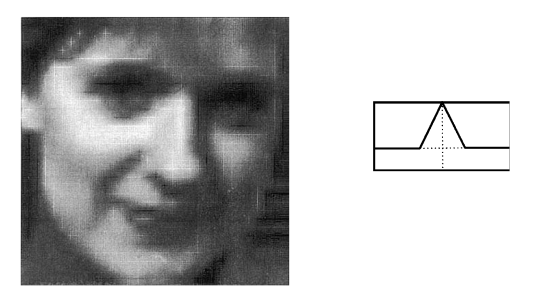
\includegraphics[totalheight=2in]{./fig/1.2.5.png}
  \caption{滤波示例} 
  \label{fig:sinc5}
\end{figure}

\begin{figure}[htbp]%[htbp]
  \centering
  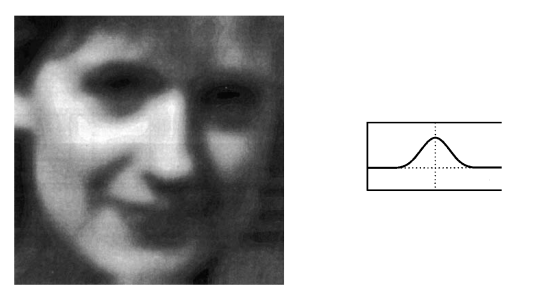
\includegraphics[totalheight=2in]{./fig/1.2.6.png}
  \caption{滤波示例} 
  \label{fig:sinc6}
\end{figure}

\begin{figure}[htbp]%[htbp]
  \centering
  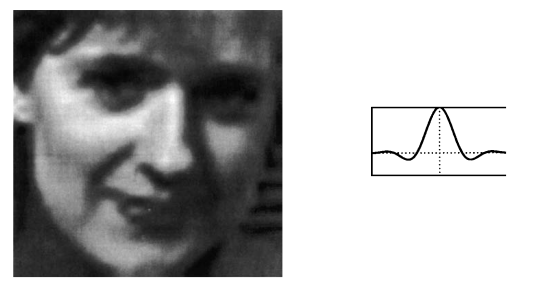
\includegraphics[totalheight=2in]{./fig/1.2.7.png}
  \caption{滤波示例} 
  \label{fig:sinc7}
\end{figure}

\begin{figure}[htbp]%[htbp]
  \centering
  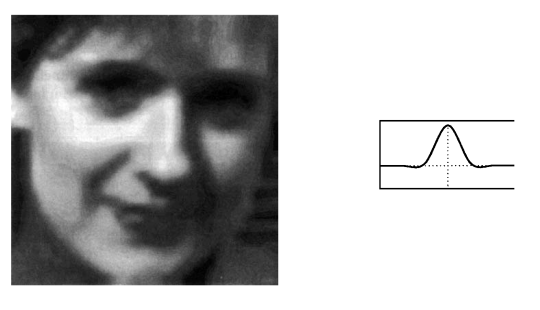
\includegraphics[totalheight=2in]{./fig/1.2.8.png}
  \caption{滤波示例} 
  \label{fig:sinc8}
\end{figure}

然后将相同的过程应用于图像的列—首先根据垂直比例因子(可能与水平比例因子不同)预计算过滤器的贡献,然后处理从中间(水平比例)图像到最终目标图像的列。

在附录中提供的源代码中,给出了许多过滤器函数,可以很容易地添加新的函数。zoom()函数以所需过滤器的名称和过滤器支持作为参数。图\ref{fig:sinc4}到图\ref{fig:sinc8}显示了不同滤波器对样本图像的影响,以及每个滤波器函数的脉冲响应图。

样本图像在两个方向上都按比例放大了12倍。图\ref{fig:sinc4}显示了一个框过滤器,它相当于直接复制像素值,因为它显示了相当多的平铺或“锯齿”。图\ref{fig:sinc5}显示了三角形或Bartlett滤波器,相对于方框来说是一个相当大的改进,计算仍然简单,但仍然有明显的过渡线。图\ref{fig:sinc6}显示了一个三次b样条,它没有产生尖锐的过渡,但是它的宽度导致了过度的模糊。三角形和b样条函数分别通过盒形滤波器与自身卷积1次和3次来计算。图\ref{fig:sinc7}显示了Lanczos 3滤波器,一个在$-3$到$+3$范围外衰减为零的$sinc$函数,它显示了在完全sinc函数时出现的过度的“振铃”效应。图\ref{fig:sinc8}显示了Mitchell滤波器($B = \frac{1}{3}, C =\frac{1}{3} $),一个没有急剧过渡的三次函数,以及“振铃(ringing)”和“模糊(blurring)”效果之间的一个很好的折衷。

See also G1, 147; G1, 166; G3, A.1.

\newpage
\section{位图缩放操作的优化}
\begin{center}
\small{
Dale Schumacher\\
St. Paul Minnesota}
\end{center}

这一节描述了一系列位图缩放操作的优化。我们没有给出一般的缩放算法,而是利用了几个特定于应用程序的限制,这些限制允许显著减少执行时间:每像素图像的位、已知的源和目标位图大小、以及位压缩的水平光栅存储和显示格式。示例应用程序是在典型的视频监视器上显示传真位图图像。

我们首先假设在内存中有源FAX,未压缩,存储为8位字节,每个字节的高阶位表示沿水平行的一组8个字节中最左边的像素。此外,在选择示例缩放因子时,我们假设源FAX的分辨率在两个方向上都是200点每英寸。如果数据是常用的200 × 100 dpi格式,我们可以通过复制每个扫描线使其为200 × 200 dpi,这是我们在解压阶段经常可以处理的任务。最初,我们将假设数据存储为与显示所用的位值匹配的白色和黑色位值。下面将讨论一种反演0位和1位含义的好方法。最后,我们假设目标位图的格式与源位图相同。

由于我们的示例图像分辨率高于您的典型视频监视器,我们将只考虑缩小图像的情况,而不是放大它。同样,我们用8来表示比例因子,$ \frac{7}{8}=87.5\%$,$ \frac{6}{8}=75\%$,$\frac{5}{8}=62.5\%$,$ \frac{4}{8}=50\%$,$ \frac{3}{8}=37.5\%$,$\frac{2}{8}=25\% $。一般算法工作如下:从源图像中取一条扫描线。对于每个字节,使用字节值作为查找表的索引,该查找表给出给定输入字节的简化位。将派生的输出位移位到累加器中。每个输入字节加到累加器的位数是基于比例因子的(例如,如果我们减少到$ \frac{5}{8} $比例,我们为每个8位输入生成5位输出)。当累加器中至少有8位时,我们从累加器中删除最左边的8位,并将它们作为输出字节写入目标扫描行。扫描线末端剩余的任何位都会被移到相应的位置并输出。许多源扫描线可以完全跳过,再次基于比例因子(例如,在$ \frac{5}{8} $的比例下,我们每8个扫描线中只处理5个,跳过3个)。

\begin{figure}[htbp]%[htbp]
  \centering
  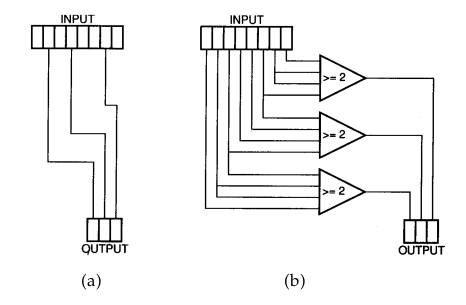
\includegraphics[totalheight=2.3in]{./fig/1.3.1.png}
  \caption{缩放操作} 
  \label{fig:1.3.1}
\end{figure}

既然已经理解了基本的算法,我们可以讨论一些有用的变化和改进过程。该算法的核心是约简查找表。如果我们需要反转最终图像中的黑白图像,一种方法是反转查找表中存储的位。然后,它将映射到1111b,而不是$00000000b$映射到$00000b$。这本质上给了我们在缩放期间免费的光度反演。类似地,通过仔细创建查找表,我们可以解决另一个问题,同样是免费的。如果我们缩小到$\frac{3}{8}$的比例,我们将在每8位中寻找3个来输出。图\ref{fig:1.3.1}a显示了这样做的最简单的方法。一个更好的方法是模拟一种对源比特进行滤波或加权平均的形式,如图\ref{fig:1.3.1}b所示。由于查找表可以在编译时创建,所以使用更复杂的算法创建表的计算成本与运行时性能无关。为了进行适当的过滤缩放,我们真的应该跨相邻扫描线和跨字节边界应用过滤器。由于这些操作会带来很高的运行时成本,并且以有限的方式应用过滤,我们可以在没有额外成本的情况下展示改进,所以我们做的是便宜的事情。即使在这些限制条件下,使用滤波也比直接对输入进行子采样要好,如图\ref{fig:1.3.1}a所示。

您喜欢的任何类型的传递函数都可以以同样的方式应用,在8位跨度的限制内,并且仅以黑白作为输入值。您甚至可以做一些事情,如反转位的顺序,这可以与不同的存储顺序一起使用,以使图像从左到右翻转,或将其旋转180度(以防有人将图像倒过来输入扫描仪)。将表扩展到16位,这将占用128Kb的内存,而不是8位表使用的256b,从而提供了更大的灵活性。使用16位时,您可以使用更大的跨度,并且可以选择16倍而不是8倍的比例因数,这可能会使您的视频显示尺寸更匹配。这些技术以及附录中给出的示例代码只是简单的构建块。检查您自己的应用程序的约束,以找到更多应用这些原则和提高代码性能的方法。

See also G1, 147; G1, 166; G2, 57; G2, 84.



\newpage
\section{一个简单的减色滤镜}
\begin{center}
\small{
Dennis Bragg\\
Graphics Software Inc.\\
Bullard, Texas}
\end{center}
\subsection*{介绍}
提出了一个简单的滤波器,将一个24位的彩色光栅图像减少到15位有效位,并消除了可见的颜色步进问题。所得到的图像可以直接显示在16位帧缓冲器上,或用作颜色量化方法的输入,以进一步减少图像中的颜色数量。

光栅图像通常存储为一个24位像素数组,8位分配给每个红、绿、蓝(RGB)组件。每个RGB组件包含256种可能的强度级别。图1(见彩色插入图)是一个24位图像,使用了2215种不同的颜色。注意彩色球平滑连续的阴影。

不幸的是,能够显示24位彩色图像的帧缓冲区并不总是可用的。使用8位像素作为256色彩色地图索引的彩色显示器被广泛使用。颜色量化方法(Gervautz和Purgathofer, 1990)常用于减少24位图像中使用的颜色数量,以便在8位设备上准确显示。

每像素可以显示16位颜色的帧缓冲器(每个RGB组件5位,加上一个属性位)也变得越来越便宜。在16位帧缓冲区上显示24位图像的典型解决方案是屏蔽每个RGB组件的三个最不重要的位。这种方法将每种颜色的256个强度级别减少到只有32个级别。

一个发生在减色平滑阴影图像的问题是颜色步进。在原始24位图像中,亮度从暗到亮连续变化的区域,在16位或8位帧缓冲区中显示时,通常会出现明显的亮度级步骤。在第2页(见彩色插入图)中,第1页的图像使用Gervautz和Purgathofer的颜色量化方法减少到256色。由于可供选择的颜色数量有限,请注意踏在球上的颜色。

该宝石通过一个加权随机量来改变每个像素RGB组件的强度级别,从而解决了颜色步进问题。方差量的加权方式这种方法的结果图像中任何像素局部区域的平均值非常接近源图像的实际24位颜色。

结果图像每像素包含15个有效的颜色位,每个RGB组件包含5个有效的颜色位。图像可以直接显示在16位帧缓冲区上,或用作颜色量化方法的输入,以进一步减少颜色的数量。得到的图像有一些“颗粒”的外观,但比可见的颜色梯度要少得多。

\subsection*{滤波器}

过滤器分别考虑每个像素的RGB组件。将一个分量的256个强度等级划分为32个相等的区域。每个区域覆盖8个强度等级。第一个区域的强度等级为0,下一个区域的强度等级为8,以此类推。

RGB组件的强度将被设置为这些区域之一。如果将组件设置为最接近的强度级别,得到的图像仍然会显示颜色步进。相反,强度除以8(或模量)的余数被确定。这给出了一个从0到7的数字。生成一个范围为0到8的随机数,并与余数进行比较。如果余数小于或等于随机数,则分量强度增加8。这具有以一种随机的方式改变组件的效果,但偏重于最接近的强度水平。

接下来,根据用户提供的噪声水平,将一些随机噪声添加到组件强度中。噪音的添加消除了任何残留的色彩踏步,否则可能是显而易见的。最后,组件较低的3位被屏蔽,将每像素的有效位数减少到15。

这个过程产生的RGB组件与原始的24位组件有很大的不同。然而,图像任意局部区域的像素分量的平均强度与原始图像的平均强度非常接近。在第三张图中(见彩色插入图),首先对原始的24位图像进行滤波处理,然后采用与图2相同的方法将图像压缩到每像素8位。
\subsection*{实现}
这个过滤器是用函数rgbvary()实现的。该函数需要四个参数:一个由待处理像素的RGB组件组成的三个字符数组(RGB),一个指定所需噪声级别的整数(noise\_level),以及像素的$x$和$y$位置($x$和$y$)。

该函数返回源RGB数组中修改后的RGB组件。噪音等级可以从0(无噪音)到8(吵闹!)2级的噪音在实践中效果很好。

像素的x和y位置由两个宏(jitterx和jittery)使用,它们生成随机数。抖动宏基于GRAPHICS GEMS中的抖动函数(Cychosz, 1990)。使用抖动的优点是它总是在特定的$x$, $y$位置上以相同的幅度变化一个像素。当你在动画中减少几帧的色彩时,这是很重要的。使用标准的随机数生成器将在动画播放时产生“雪花”效果。jitter函数消除了这个问题。

在调用rgbvary()以初始化jitter宏使用的查找表之前,必须调用函数jitter\_init()。这个过程使用标准的C函数rand()来填写表格。

\subsection*{总结}

一种滤波器被提出,以减少24位图像为15有效位每像素。该程序消除了颜色步进的问题,但代价是外观略有颗粒。生成的图像可以直接显示在16位帧缓冲上,或用作颜色量化方法的输入,以进一步减少颜色。

\begin{figure}[htbp]%[htbp]
  \centering
  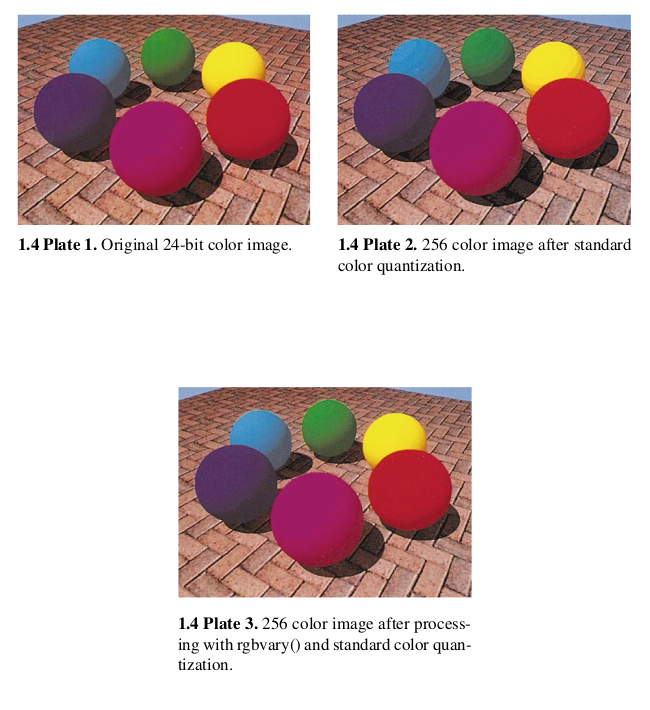
\includegraphics[totalheight=5in]{./fig/1.4.png}
  \caption{颜色滤波} 
  \label{fig:1.4}
\end{figure}

\newpage
\section{从抽样数据得到的紧凑等高线}
\begin{center}
\small{
Dennis Bragg\\
Graphics Software Inc.\\
Bullard, Texas}
\end{center}


\subsection*{问题}
包括医学成像、地震学和气象学在内的许多领域的数据,都是在一个大立方体网格的顶点上采集的一组测量数据。在这些领域中,从数据立方体生成可视化表示的技术非常重要。许多常见的可视化技术将数据值视为连续函数$F$的样本函数值,并对某些$c$生成$F(x, y, z) = c$的分段平面近似,即函数的等值线。最初的《图形瑰宝》之一,“从采样数据定义表面”,调查了几种最著名的从数据立方体生成等高线的技术(Hall, 1990)。

在本文中,我们将对该类型的所有技术进行增强。这种增强减少了任何等高线近似的元素数量,并改善了元素的形状。第一个改进通常将表示的大小减少约$50\%$,允许更快的重新显示并减少内存需求。第二种方法通过避免在许多照明模型中造成不希望看到的阴影影响的狭窄元素,从而得到质量更好的图片。

\subsection*{基于立方体的轮廓}
一些作者提出了大致类似的方法,可以从立方体数据网格中创建可视化的等高线。这些方法分别处理每个立方体上的数据,并利用沿立方体边缘的线性插值来计算位于等高线上的点集合。在Lorenson和Cline的Marching Cubes算法(Lorenson和Cline, 1987)中,这些交点通过表查找来连接成边和三角形,表查找的基础是定义立方体顶点的值$F(x, y, z) - c$的符号。

不幸的是,这种方法并不能保证轮廓的连续性,因为共享一张带有混合符号的脸的相邻立方体可以以不同的方式划分(Durst, 1988)。其他人提出了另一种方法,通过对模糊人脸中心的函数进行采样来消除这种情况的歧义(Wyvil等人,1986)。我们称之为这样的方法,通过沿着三次网格边缘的线性插值计算出轮廓的顶点,基于边缘的插值方法。

基于边缘的插值方法的另一个问题是,它们产生的表面网格可能非常不规则,即使是简单的三元数据。这些不规则性包括微小的三角形(当轮廓通过立方体网格的顶点时产生)和狭窄的三角形(当轮廓通过网格的边缘时产生)。根据我们的经验,在某些曲面网格中,这种三角形可以占到三角形的$50\%$。这些形状糟糕的元素通常会降低渲染算法和有限元分析应用于网格的性能,而对近似的总体精度贡献很小。

\subsection*{紧凑立方体}
这个章节的贡献是一种通用的技术,用于从基于边的插值中消除近简并三角形的问题。该技术背后的想法很简单:当网格的一个顶点靠近表面时,将网格“弯曲”一点,这样顶点就位于表面上。小三角形坍缩成点,小三角形坍缩成边,只剩下形状良好的大三角形。本文的其余部分概述了这一理念的实现;有更详细的解释(Moore和Warren, 1991)。

对数据立方体应用任何基于边的插值算法,并在此过程中,记录沿着立方体边缘生成的每个顶点,该顶点附近的立方体网格的点。我们称这个顶点为它最近的网格点的卫星。如果顶点位于一条边的中点,则可以使用这条边的任意端点,只要共享这条边的所有其他立方体使用同一个端点。当算法的这一阶段完成后,就得到了等高线的三角剖分S和一个离三角剖分的每个顶点最近的网格点。
\begin{figure}[htbp]%[htbp]
  \centering
  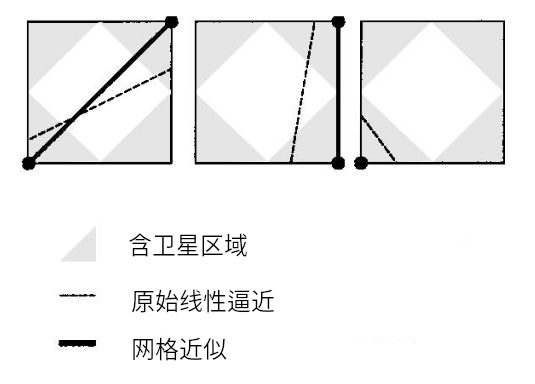
\includegraphics[totalheight=1.8in]{./fig/1.5.1.png}
  \caption{二维案例表紧凑型立方体} 
  \label{fig:1.5.1}
\end{figure}

\begin{figure}[htbp]%[htbp]
  \centering
  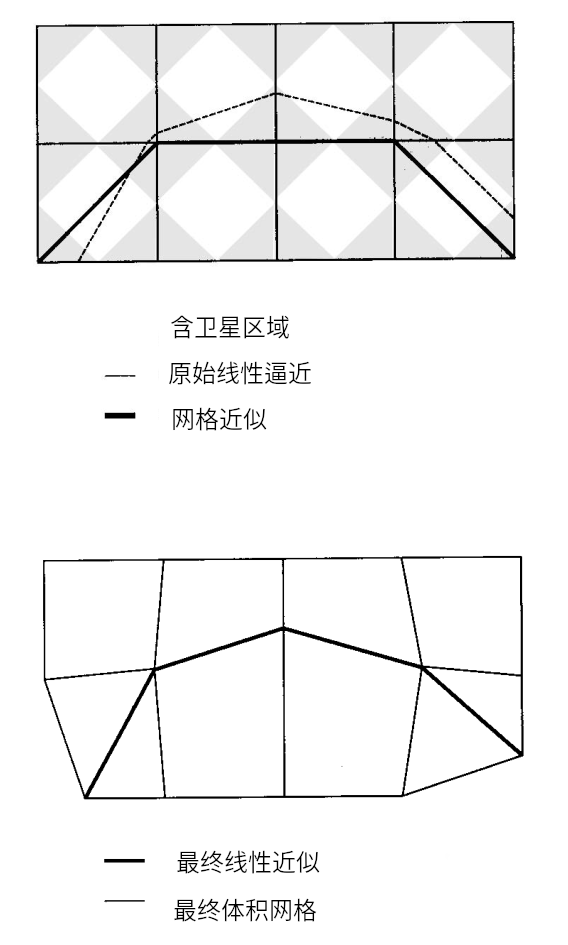
\includegraphics[totalheight=3in]{./fig/1.5.2.png}
  \caption{一个二维立方体的例子} 
  \label{fig:1.5.2}
\end{figure}



为了得到一个新的、更小的等值线近似值,请采用以下步骤(算法\ref{algo:approximation} ):
\IncMargin{1em}
\begin{algorithm} 
\SetKwData{Left}{left}
\SetKwData{This}{this}
\SetKwData{Up}{up} 
\SetKwFunction{Union}{Union}
\SetKwFunction{WritePixel}{WritePixel}
\SetKwFunction{Abs}{abs}
\SetKwFunction{Floor}{floor}
\SetKwFunction{Ceiling}{ceiling}
\SetKwFunction{Sign}{sign}
\SetKwFunction{ReadPixel}{ReadPixel}
\SetKwFunction{SetColor}{SetColor}
\SetKwFunction{FindCompress}{FindCompress} 
\SetKwFunction{Filter}{filter}
\SetKwFunction{AddContributor}{add\_contributor}

\SetKwInOut{Input}{输入}
\SetKwInOut{Output}{输出}

\SetKwData{EdgeSet}{EdgeSet}
\SetKwData{Point}{point}
	
	%\Input{} 
	%\Output{}
	 \BlankLine 
	 \BlankLine
	 
	 
	 
	 %\tcp{从(x1, y1)到(x2, y2)在第一个八边形内画一条线;所有变量都是整数}
	
	\For{ each triangle $T$ in $S$ }{
		\If{the vertices of $T$ are satellites of distinct gridpoints}{
			produce a triangle connecting the gridpoints\;
		}
		\Else{
			$T$ collapses to a vertex or edge so ignore it\;
		}
		\For{ each gridpoint $g$ of the new triangulation }{
			displace $g$ to the average position of its satellites;
		}
	}
	
 	 	  \caption{等值线近似值}
 	 	  \label{algo:approximation} 
 	 \end{algorithm}
\DecMargin{1em} 

\begin{figure}[htbp]%[htbp]
  \centering
  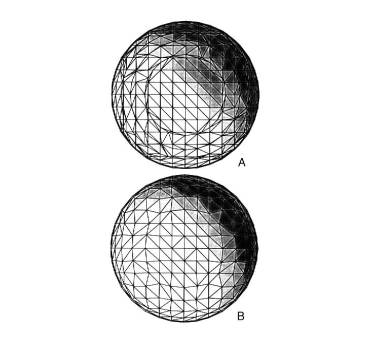
\includegraphics[totalheight=1.8in]{./fig/1.5.3.png}
  \caption{球面的两个近似值} 
  \label{fig:1.5.3}
\end{figure}

\begin{figure}[htbp]%[htbp]
  \centering
  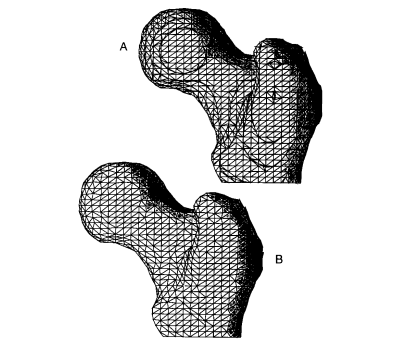
\includegraphics[totalheight=1.8in]{./fig/1.5.4.png}
  \caption{两个股骨头的近似图} 
  \label{fig:1.5.4}
\end{figure}

该方法的第一步是定义新网格连接点的拓扑结构。在S中,一个特定网格点的所有卫星被合并成结果网格中的单个顶点。因此,当一个网格点被“切掉”时产生的小三角形被折叠到网格点上。当两个顶点非常接近同一个网格点时产生的窄三角形被折叠成一条边。图1以两个维度说明了这一点。从这个角度来看,如果原曲面网格是连续的,那么算法第一步生成的网格也必须是连续的。

在第二步中,网格的顶点被平移到原始等高线上或附近。由于每个新的顶点位置被选择为位于原始轮廓上一小簇点的平均位置,新的近似通常只与原始轮廓稍微偏离。

图\ref{fig:1.5.2} 说明了这种方法应用于二维网格。上面的部分说明了第一步的结果。下面的部分说明了第二步的输出。图形上部的短边已折叠成下部的顶点。

实际上,这种方法效果很好,将三角形的数量减少了$40\%$到$60\%$。图\ref{fig:1.5.3} 显示了一个球体由游行立方体(a)和相同的球体后紧凑的立方体(B)的应用。图\ref{fig:1.5.4}显示了一个人类的股骨,最初作为CT数据,为波状外形的游行立方体(a)和紧凑的立方体(B)。在每个例子中,三角形的数量减少了使用紧凑的数据集,其余三角形的形状也得到了明显的改善。

正如这里所描述的,紧凑立方体产生的轮廓可能有几个不受欢迎的特征。首先,最终轮廓的边界可能不在定义的立体网格的边界上。第二,通过公共网格点附近的轮廓的两个不相交的薄片可以在该网格点融合。Moore和Warren(1991)描述了对Compact Cubes的简单修改,解决了这些问题。


See also G1, 552; G1, 558; G2, 202.

\newpage
\section{从位图生成等值线}
\begin{center}
\small{
Tim Feldman\\
Island Graphics Corporation\\
San Rafael, California}
\end{center}


本节提出了一种算法,该算法遵循采样数据数组中的轮廓边缘。它使用Freeman链编码生成一个向量列表,描述轮廓的轮廓。

假设您有一个已采样或“数字化”成灰度像素矩形阵列的地形图。不同的像素值对应不同的地形高程。该算法可用于生成以等高线表示地形高程的“地形图”。附录中给出了一个遵循一条轮廓线的示例程序(\textit{contour.c})。

该算法能够处理包含单个样本点的等高线、围绕不同海拔区域的等高线、不形成闭合曲线的等高线、以及形成交叉曲线、形成环路的等高线。在所有情况下,它遵循轮廓的最外层边缘。给定阵列中高程轮廓的初始点,该算法找到轮廓的边缘。然后顺时针方向沿着这条边走,直到它回到起点。沿着每个方向向量描述了从路径上的一个像素到路径上的下一个像素的方向。路径上的所有像素都是近邻。因此,向量可以被认为是传统二维向量的方向部分,其长度部分总是等于一个像素。这样的向量列表被称为“弗里曼链”,以其创始人Herbert Freeman命名(Freeman, 1961)。图\ref{fig:1.6.1} 显示了定义从一个像素到其邻居路径上的八个可能方向的值。本例中使用的像素阵列如图\ref{fig:1.6.2}a所示;图\ref{fig:1.6.2}b显示了示例程序的输出。算法从样本$x = 3$, $y = 2$开始,寻找$\text{高程}= 200$的等高线边缘并跟踪。

\begin{figure}[htbp]%[htbp]
  \centering
  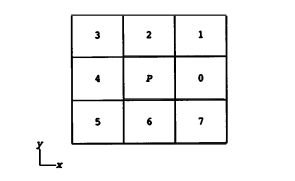
\includegraphics[totalheight=1.8in]{./fig/1.6.1.png}
  \caption{从点P到它的八个邻居的方向向量。} 
  \label{fig:1.6.1}
\end{figure}

\begin{figure}[htbp]%[htbp]
  \centering
  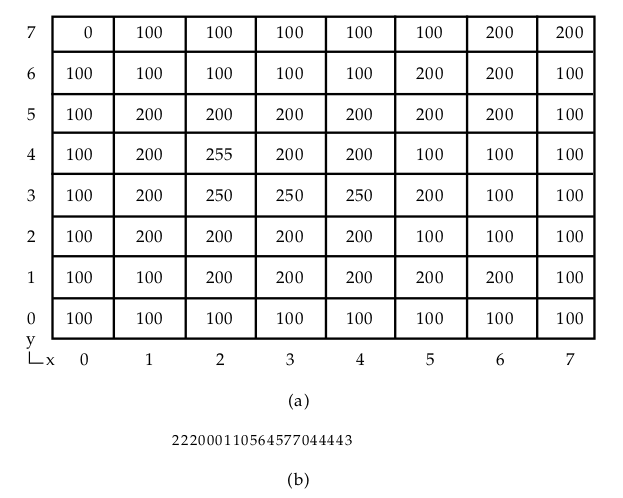
\includegraphics[totalheight=3in]{./fig/1.6.2.png}
  \caption{a)标高数据采样样例。\\b)绘制$\text{高程}= 200$等高线轮廓的22个点向量。} 
  \label{fig:1.6.2}
\end{figure}

该算法的核心在于知道如何以顺时针方向沿着轮廓的方式选择邻居。测试图\ref{fig:1.6.2}a,并想象您从$x = 1$, $y = 2$的采样点出发,沿着高程= 200的等高线边缘行走。为了顺时针移动轮廓线,你的第一个移动应该是$x = 1$, $y = 3$处的样本。你走在自己轮廓的边缘;在你的左边是危险的悬崖,它向下坠落到一个较低的高度。当你沿着轮廓走的时候,注意你的头部是变化的,但是悬崖总是在你的左边。在选择下一步的时候,你总是试着向前走,向左走,而不是走下悬崖。如果你不能向前移动到你的左边,你试着顺时针方向:直走。如果不行,你试着顺时针方向向前,向右,等等。如果你发现自己在一个海角上,你顺时针方向的方向会让你掉头,重新走一段路。最终,你将完全沿着轮廓移动,然后回到你的起点。

算法的工作原理是一样的。\textit{build()}过程构建围绕轮廓边缘移动时所采取的方向的Freeman链。\textit{build()}调用\textit{neighbor()}过程来获取路径上的下一个邻居。\textit{neighbor()}反过来调用\textit{probe()}来查找该邻居。最低级的过程是\textit{in\_cont()},它只是简单地测试给定的样本是否在轮廓中。请注意,采样数据的整个数组不需要立即放入内存;\textit{in\_cont()}可以修改为随机访问脱机存储,如果需要的话。

\textit{neighbor()}中的\textit{last\_dir}变量维护\textit{neighbor()}的方向感。检查图3,看看邻居()过程是如何实现上面描述的“尝试向前移动并向左移动”的步骤的。假设你从样本a到达样本P,那么\textit{last\_dir}是2,而样本C总是在等高线之外,所以第一个探测的邻居是D。从P到D的方向是3;\textit{new\_dir←last\_dir + 1}。

\begin{figure}[htbp]%[htbp]
  \centering
  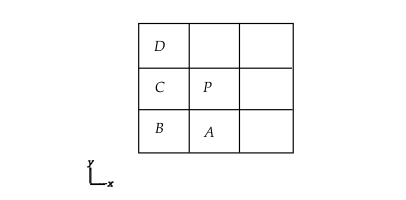
\includegraphics[totalheight=1.5in]{./fig/1.6.3.png}
  \caption{从P点通过A或B点移动到D点} 
  \label{fig:1.6.3}
\end{figure}

现在假设您从b到达了P, \textit{last\_dir}是1,C仍然在等高线之外,D仍然是要探测的第一个邻居。P到D的方向仍然是3;\textit{new\_dir←last\_dir + 2}。

请注意,当\textit{last\_dir}等于0、2、4或6时,到达P点的情况都是全等的(它们只是被旋转了90度)。类似地,\textit{last\_dir} = 1、3、5和7的情况都相等。因此,\textit{neighbor()}使用的简单规则是将\textit{new\_dir}设置为\textit{last\_dir + 1}(如果\textit{last\_dir}为偶数),或将其设置为+ 2(如果\textit{last\_dir}为奇数)。当然,\textit{new\_dir}的范围必须保持在0到7之间,因此加法对8取模。

E的取值范围从0到7,所以加法对8取模。唯一剩下的微妙之处是如何正确地选择第一个移动,以便以顺时针方向围绕轮廓开始。这是很容易实现的:算法,当给定一个起点在轮廓的任何地方,在轮廓向左移动,直到它遇到边缘。这保证了路径从边缘开始。它还保证了初始排列如图3所示:路径从样本P开始,C处的邻居不在等高线中,并且\textit{new\_dir}的值应为3。这意味着\textit{last\_dir}的初始值应该是1。算法在\textit{build()}过程中设置它。

这个示例程序是为了演示Freeman链背后的思想而编写的,但它的存储效率并不高。链表中的每个成员占用一个整数和一个指针。但正如Freeman在他最初的工作中指出的,每个方向向量编码只需要三个比特。使用三位的实现将使用一个大的内存块而不是链表,并且将有将方向向量链打包到块中的过程,并按顺序提取它们。为了确定应该为保存轮廓中所有方向向量的块分配多少内存,将使用轮廓跟踪算法的简化版本。它会沿着轮廓线计算描述完整路径所需的方向向量的数量,但它不会存储方向向量。一旦确定了矢量的数量,就会分配内存,调用主算法重描轮廓,并将方向矢量打包到内存块中。

前面的方法比示例程序更有效,但它用速度换取了内存空间。第三种方法仍然允许轮廓具有任意长度,同时有效地使用内存空间,同时保持良好的速度。它通过消除预扫描步骤来实现这一点。对于使用大数据集或不保存在内存中的数据集的实现来说,这是一个重要的考虑因素。方法是使用一个简单的链表,就像示例程序一样。但是,列表中的每个成员都有一个分配的内存块,而不是一个整数。这个块包含许多方向向量,每一个都被压缩成3个比特。更多的数据块将被分配,并根据需要链接到列表中,因为轮廓是遵循的。包装和提取带菌者将需要程序,而且必须保持额外的管理资料,以便使一切都处于控制之下。这种技术为链表中的指针使用了少量空间,但仍然比示例程序的内存效率高得多。这种方法的权衡是在实际编程中经常遇到的问题:为了在保持速度的同时节省存储空间,会增加程序的复杂性。

最后,一些实现可能根本不需要在内存中保存轮廓的表示;它们可以简单地将方向向量写入顺序访问磁盘文件或某些输出设备或并发进程。在这种情况下,示例程序的\textit{build()}过程将被修改。

See also G3, A.5.

\newpage
\section{合成黑白位图}
\begin{center}
\small{
David Salesin   \hspace{25ex}                 Ronen Barzel\\
\hspace{10ex} Cornell University    \hspace{5ex}        and  \hspace{3ex}   California Institute of Technology\\
\hspace{3ex} Ithaca, New York           \hspace{20ex}           Pasadena, California}
\end{center}

\subsection*{介绍}

典型的位图编码黑白像素。添加一个辅助位图允许我们表示透明的像素。这种两位表示对于非矩形或有孔的黑白图像很有用。它还为组合位图提供了一组更丰富的操作。我们用布尔值对$(\alpha, \beta)$编码三个可能的像素值,如下所示:



\begin{center}
\begin{tabular}{ccl}
\hline
$\alpha$ & $\beta$ & Meaning \\
\hline
1 & 0 & Black \\
1 & 1 & vvnite \\
0 & 0 & Transparent \\
0 & 1 & Undefined \\
\hline
\end{tabular}
\end{center}


\subsection*{Compositing Bitmaps}

我们可以使用合成操作$\mathrm{R} \leftarrow \mathrm{P}\quad \mathbf{op} \quad \mathrm{Q}$
将两个像素$\mathrm{P}=\left(\mathrm{P}_{\alpha^{\prime}}, \mathrm{P}_{\beta}\right)$
和$\mathrm{Q}=\left(\mathrm{Q}_{\alpha^{\prime}} \mathrm{Q}_{\beta}\right)$
组合成一个新的像素$\mathrm{R}=\left(\mathrm{R}_{\alpha^{\prime}} \mathrm{R}_{\beta}\right)$,如表一所示。


该表是将全彩合成代数(Porter and Duff, 1984)简化为两个位域(Salesin and Barzel, 1986)。注意,表中$\mathrm{R}_{\alpha}$和$\mathrm{R}_{\beta}$的方程现在是布尔公式:and被写成乘法,OR写成加法,XOR写成$\oplus$。布尔操作可以使用一系列标准的“bitblt”操作一次对整个位图执行。根据操作的不同,所需的bitblt总数从2到4不等。



\begin{table}[htbp]
\begin{center}
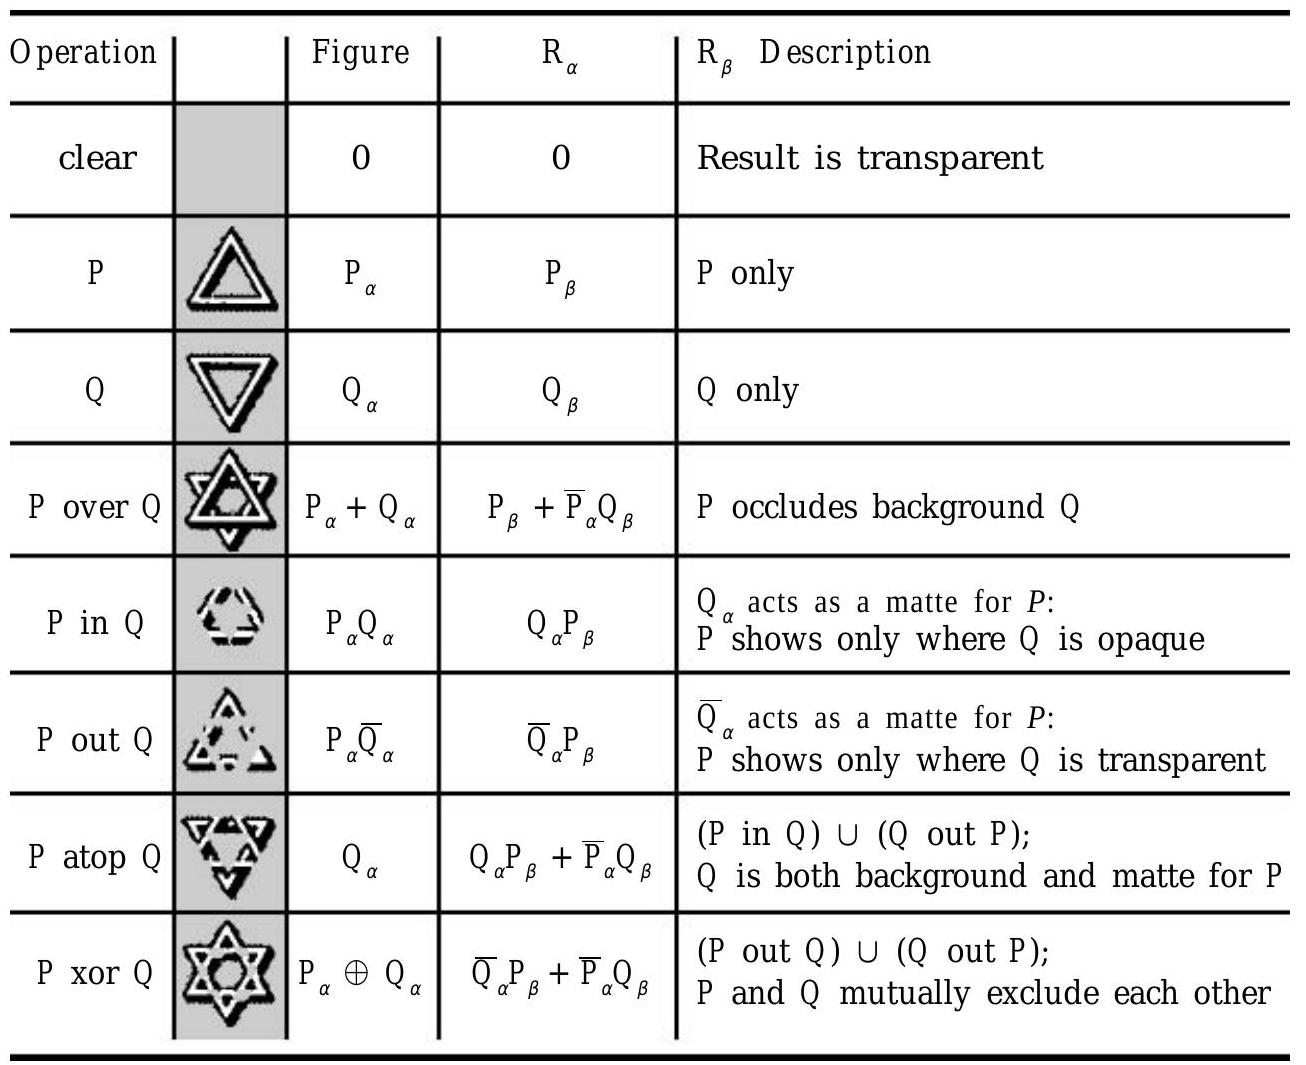
\includegraphics[max width=4in]{2022_11_30_0cbb01a33d99487fc27fg-066}
\end{center}
\caption{位图合成操作}
\end{table}

表中的数字描述了操作对两个示例位图$\mathrm{P}$和q的影响。在这些数字中,使用灰色调表示结果中的透明区域。


over运算符用于将非矩形黑白位图置于现有图像之上——它非常适合绘制游标。in和out操作符允许一个位图作为另一个位图的哑光—例如,如果$P$是一个“砖”纹理,而Q是一个“建筑”,那么P in Q就会用砖对建筑进行贴片。如果一个位图同时充当另一个位图的哑光和背景,那么atop操作符很有用——例如,它允许将一小块纹理增量地绘制到现有位图上。


See also G1, 210.


\newpage

\section{计算机动画的$2\frac{1}{2}D$景深模拟}

\begin{center}
\small{
Cary Scofield  \\
Hewlett-Packard Company\\
Chelmsford, Massachusetts           }
\end{center}

\subsection*{介绍}

景深被定义为在光学透镜系统中包围焦平面的区域,在该区域内物体保持确定的焦质量。长期以来,摄影师和电影摄影师一直利用相机镜头和光圈的这一方面,将观众的注意力从感兴趣的领域以外的区域引导到图像的特定部分。正因为如此,在计算机动画系统中加入景深效果是非常有利的。

这个gem描述了一个$2 \frac{1}{2}$-D的景深算法,用于模拟计算机生成的动画中的焦点变化。这种特殊的算法实际上独立于任何隐藏面去除技术。我们根据深度将3d场景分层为独立渲染的不相交对象组。生成的图像经过滤波模拟景深,然后通过合成后处理重新组合成单幅图像。当逐渐改变滤镜应用于动画序列的连续帧时,其效果是将观看者的注意力从场景的一个深度面拉到另一个深度面。


\subsection*{相关工作}
以前模拟景深的尝试涉及使用针孔相机模型(Potmesil和Chakravarty, 1982)。然而,该算法没有考虑到透镜表面提供了连续的环境不同视图这一事实。分布射线追踪(Cook et al., 1984)克服了这一缺陷,但将该技术嵌入到渲染过程中。我们的算法可以被认为是这两种方法的折中:虽然我们不整合阴影和景深,但我们确实以一种受限的方式结合了表面可见性和景深。


\subsection*{算法}
我们的方法本质上是一个三个阶段的过程:

\begin{enumerate}
	\item 隐藏表面去除阶段:\\
	在第一个阶段中,可以手动或自动地将对象分层或聚类到前景和背景组中。每个簇或组被单独渲染成它自己的图像,每个像素的alpha通道有一个不透明度掩码(见图1,颜色插入)。这种不透明度遮罩最终在第三阶段发挥作用,但它可以在第二阶段进行修改。

	\item 滤波器后处理阶段:\\
	该阶段使用类似于指数低通滤波器的卷积掩模来模糊各种图像,以模拟景深效果。由于我们的算法与模拟透镜的焦距无关,这允许我们自由地操纵图像的模糊程度。然而,我们的目的是创造一个现实的效果,所以我们仔细选择模糊程度。还必须小心避免“渐晕”(Perlin, 1985),如果过滤算法不补偿图像边界之外的未知区域,就会出现这种现象。这是通过重新计算加权滤波器,每当卷积掩模的任何部分被图像边界剪辑。
	
	\item 合成阶段:\\
	最后,在这一阶段,我们遵循波特和达夫(1984)、达夫(1985)和麦克斯和勒纳(1985)建立的算法。第一阶段中不透明度蒙版的重要性在这里发挥了作用,因为它允许我们在将前景图像叠加到背景图像时避免混淆工件。

\end{enumerate}

\subsection*{焦距变化模拟}
正如在介绍中所述,电影摄影师长期以来一直使用焦点的变化来推动或拉观众的注意力从场景的一个部分到另一个部分(例如,从前景到背景)。这种“聚焦”是未经过滤的前景对象(“聚焦中”)与模糊的背景(“超出”焦平面)叠加的结果。因此,将观众的注意力从前景拉到背景,相当于在一系列帧中,将镜头的“焦平面”沿着光轴从前景逐渐转移到背景。因为我们不使用镜头和光圈相机模型,我们必须从一帧到一帧修改模糊滤镜的形状。假设发生焦点变化模拟的帧数是先验的,我们可以很容易地对滤波器的“模糊度”进行插值,范围从一个很小的值到一个能给我们期望的最大图像模糊度的大小。这是为前景对象做的。对于相应的背景图像,我们使用相同的插值值系列,只是顺序相反。当过滤过程完成后,两个独立的前景和背景图像流在最后一个阶段被拼接在一起,形成拍摄的最终图像帧。图b、c和d(见颜色插入)分别是由这个过程产生的动画序列的第一帧、中间帧和最后帧的例子。作为一个边注,这一过程所获得的结果与塞尔动画中偶尔使用的多平面相机系统所获得的结果非常相似(Thomas和Johnston, 198l)。


\subsection*{致谢和历史记录}
这本书是几年前与詹姆斯·阿尔沃(James Alvo)合作撰写的一篇更详细但从未发表过的论文的浓缩。作为一个历史笔记,在这个宝石中描述的焦点变化模拟被用于两个阿波罗计算机射线追踪动画公司中的第一个(即“Quest”)。

\begin{figure}
\centering
	\subfigure[由它们自己渲染的场景中的一簇物体。]{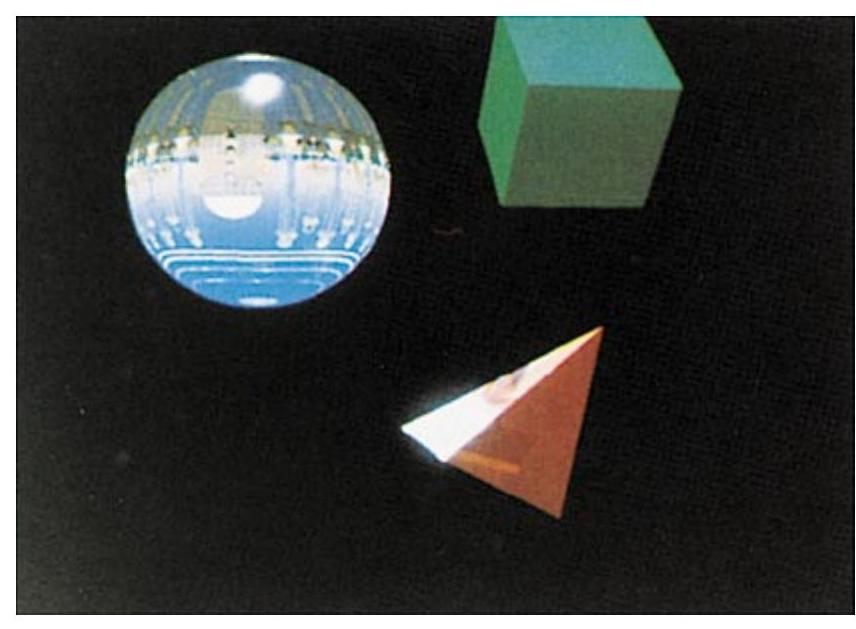
\includegraphics[max width=.35\columnwidth]{2022_11_30_0cbb01a33d99487fc27fg-070}}\hspace{5pt}
	\subfigure[前景和背景物体的合成图像。前景是“聚焦”。]{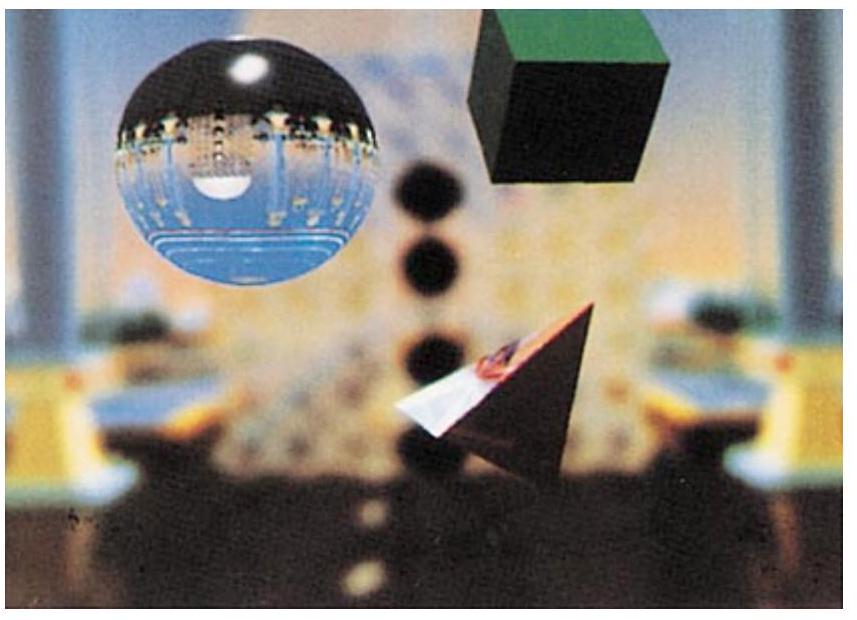
\includegraphics[width=.35\columnwidth]{2022_11_30_0cbb01a33d99487fc27fg-070(2)}}\\
	\subfigure[合成图像。前景和背景对象模糊化。]{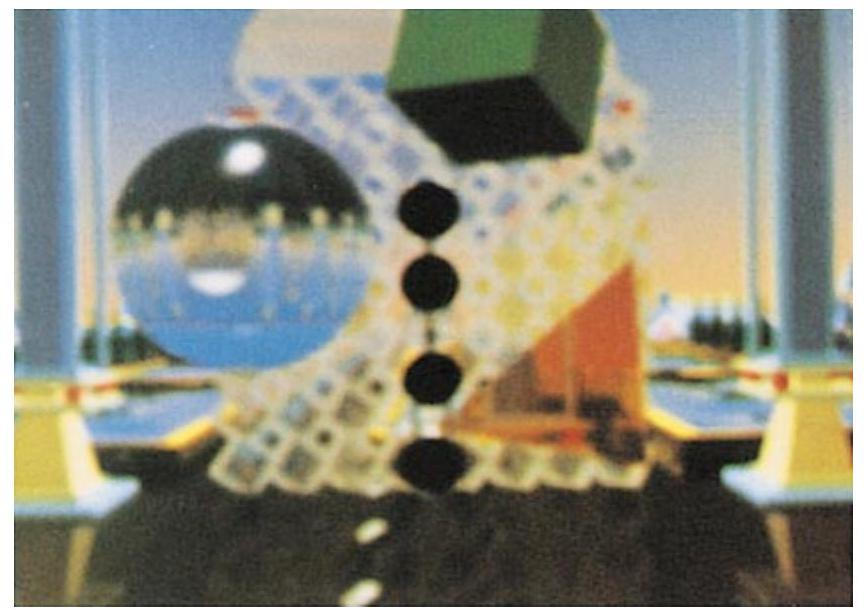
\includegraphics[width=.35\columnwidth]{2022_11_30_0cbb01a33d99487fc27fg-070(1)}}\hspace{5pt}
	\subfigure[合成图像。动画序列的最后一帧,背景对象“聚焦”。]{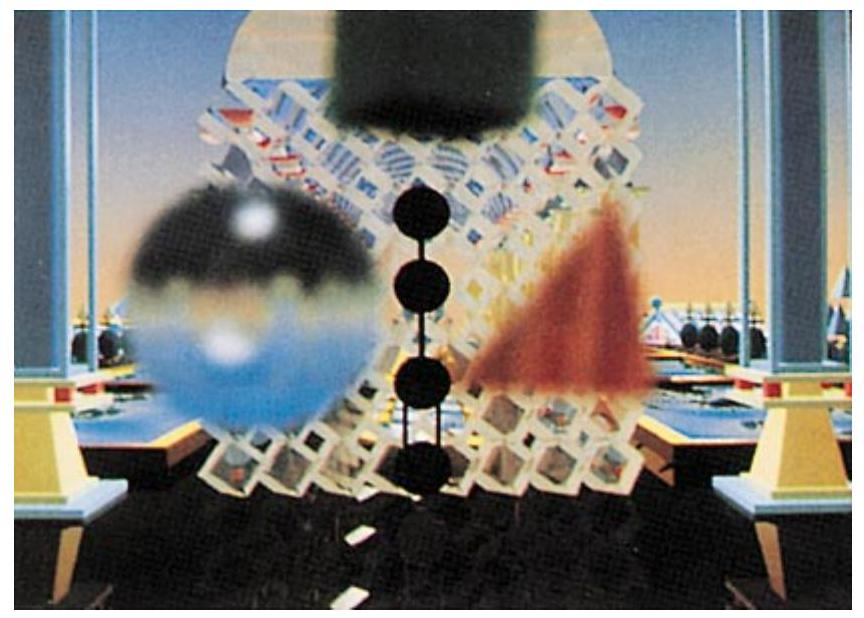
\includegraphics[width=.35\columnwidth]{2022_11_30_0cbb01a33d99487fc27fg-070(3)}}
\end{figure}

\newpage
\section{复合区域的快速边界生成器}
\begin{center}
\small{
Eric Furman  \\
General Dynamics, Electronics Division\\
San Diego, California           }
\end{center}

\subsection*{问题}
在计算机图形学的许多应用中,寻找由封闭边界定义的多个区域的轮廓是一个常见的问题。通过求一组圆的包络线可以确定一组雷达站点的二维覆盖,如图1所示。另一个例子是土地利用和城市规划中若干分区的大纲。一般来说,这类应用程序都是将兴趣区域的联合可视化。需要一种算法来找到这些区域的复合边界或包络线。换句话说,我们希望显示一组二维区域的轮廓。每个区域在二维上都是一个封闭边界。常见的区域原语是圆、多边形和椭圆,但任何其他封闭区域轮廓都可以使用所描述的技术很好地工作。在这个gem中,我们将使用圆作为我们的基本示例区域。图1到图3显示了该算法的步骤。圆集合的轮廓有许多短的连接弧或扇形。


\subsection*{其他方法}
针对多雷达站点问题的几种解决方案都采用了直接分析的方法。他们通过一系列雷达范围圆进行工作,通过将每个新圆与以前的交叉点生成的弧相交,从而创建一组弧(Bowyer and Woodwark, 1983)。不相交的圆必须带着,并与每个新圆相交。对每个新圆进行内部/外部测试,并修改弧集以删除一些弧段并添加新的弧。不幸的是,随着圆列表的增长,生成边界的时间随着圆数量的平方而增加。已经实现了一些改进,例如完全丢弃包含在其他圆中的圆,并使用边界框测试来限制更昂贵的圆/弧相交测试的数量。

\begin{figure}
\begin{center}
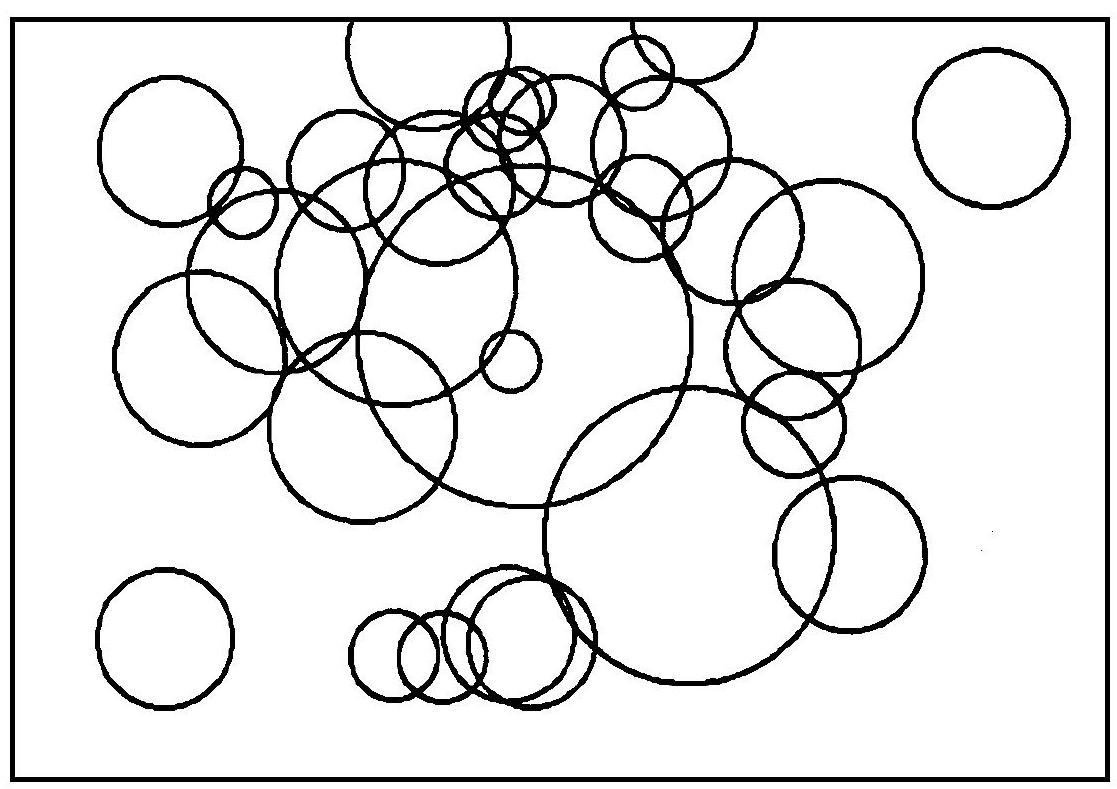
\includegraphics[max width=\textwidth]{2022_11_30_0cbb01a33d99487fc27fg-072}
\end{center}
\caption{A set of circles shown in a frame buffer.}
\end{figure}

\begin{figure}
\begin{center}
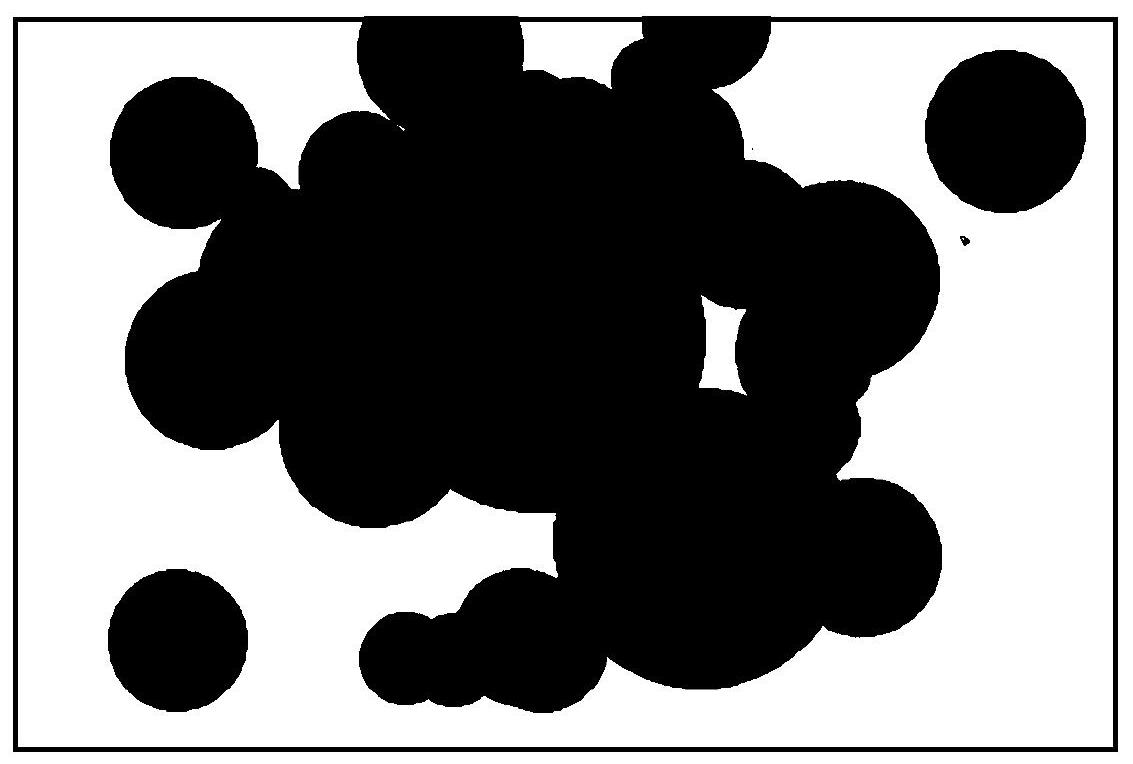
\includegraphics[max width=\textwidth]{2022_11_30_0cbb01a33d99487fc27fg-072(1)}
\end{center}
\caption{The circles of Fig. 1 after filling.}
\end{figure}


Figure 2. The circles of Fig. 1 after filling.

\begin{figure}
\begin{center}
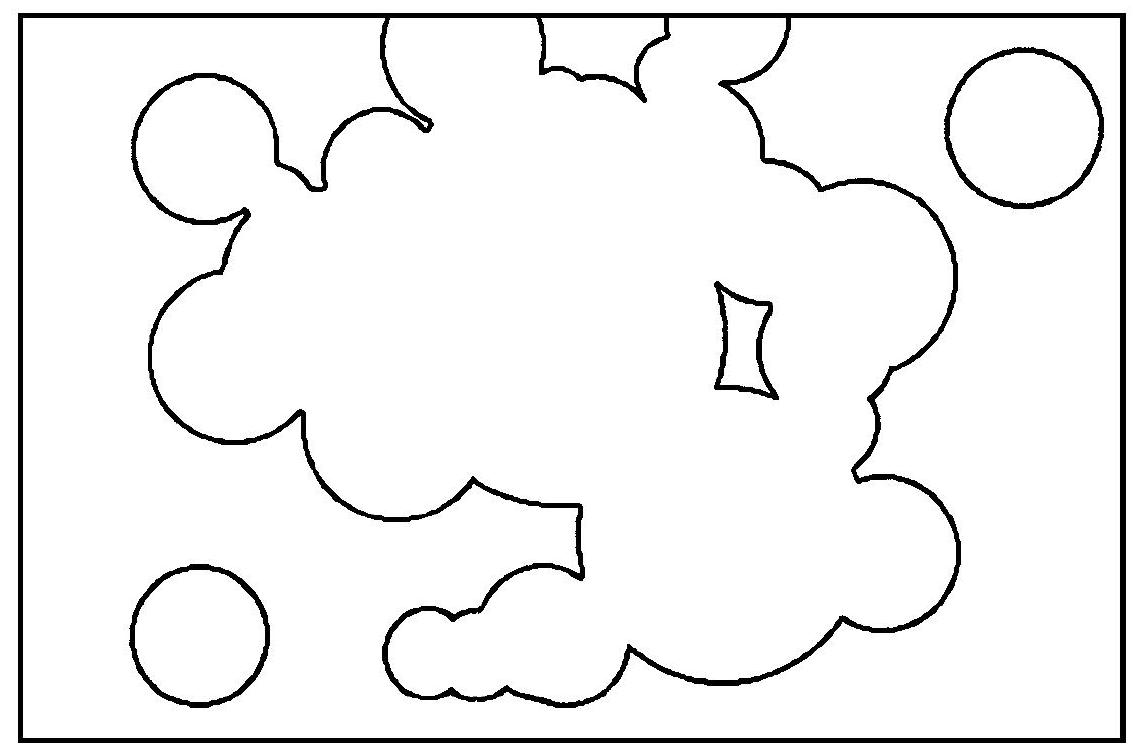
\includegraphics[max width=\textwidth]{2022_11_30_0cbb01a33d99487fc27fg-073}
\end{center}
\caption{Scallops. The envelope of Fig. 1 circles.}
\end{figure}


这种直接的分析方法适合于创建分辨率远高于典型帧缓冲区所能显示的区域边界数据集。然而,可视化一组区域的包络可以更快地完成。


\subsection*{快速生成边界}
一种混合了计算机图形学和图像处理技术的快速生成区域边界的方法。该算法由两个基本步骤组成,用于帧缓冲区的有限分辨率。首先,对于每个封闭原语,绘制填充区域并将其剪切到帧缓冲区限制。尽管我们希望只显示许多闭合对象的信封,但我们同时绘制和填充每个对象。通常绘图和填充可以通过精心的算法构造在同一个步骤中完成。其次,在整个帧缓冲区上应用侵蚀运算符来删除所有填充的内部点。没有填充的对象,侵蚀不会使它们减少到复合边界。这个过程如图1-3所示,每个圆都是独立绘制和填充的。


该算法的执行时间是所有区域的绘图和填充时间加上单道侵蚀操作的时间。在我们的示例中,这是绘制/填充所有圆所需的时间加上侵蚀它们所需的时间。当绘制单个重叠对象时,不填充先前由另一个区域填充的像素似乎可以节省一些时间。不幸的是,测试确定一个区域是否已经被填满通常比仅仅将数据写入帧缓冲区要花费更长的时间。所需的时间与所有区域的填充面积成线性增长,对于直接分析方法的平方增长率有相当大的改进。

附录II中用于生成填充圆的示例$\mathrm{C}$代码改变了计算机图形文本中给出的通常的中点圆生成算法,以创建填充圆(Foley et al., 1990)。通过调用raster\_ fill函数来填充圆,该函数直接实现了使用fill\_circle 函数中的二阶偏差生成中点圆的算法。


将填充区域侵蚀到它们的边界轮廓,查看帧缓冲区中每个像素及其最近的四个连接邻居。一个填充的像素值或颜色将被擦除为侵蚀值,只有当它的所有四个连接的邻居像素也被填充相同的值。对背景值的侵蚀将只留下以原始填充颜色绘制的边界像素。然而,侵蚀到不同的颜色将留下轮廓在原始填充值和填充内部用新的侵蚀值。在这个测试过程中使用了三个光栅缓冲区,以避免在以后计算其他像素时替换帧缓冲区中的像素,或者需要从一个帧缓冲区渲染到另一个帧缓冲区。在附录II的$\mathrm{C}$代码中,栅格缓冲区向帧缓冲区添加了一个单像素的边界。用对象的原始像素填充值填充这个边界将留下一个开放的边缘,在这个边界被剪切在帧缓冲区的边缘。当边界设置为背景值(在代码中为零)时,在发生帧边缘裁剪的地方绘制一个封闭边缘包络线。这个过程是图像处理的二值边缘检测(Gonzalez和Wintz, 1987)在计算机图形学中的一个相当简单的应用。

\subsection*{注意事项}
尽管这种技术简单快速,像大多数帧缓冲算法一样,它只能精确到最近的像素。解析解的精度将受到计算所用的算术精度的限制。


对于圆,可以通过生成一个固定圆的栅格跨度宽度表来提高速度。直径应该至少是帧缓冲区最大尺寸宽度的两倍,以保持在Nyquist区间内。然后,该表可用于任何所需圆大小的比例宽度查找。表查找消除了进一步的圆生成,但仍然必须执行剪切和填充操作。对于任何直接可伸缩和未旋转的区域,也可以获得类似的表好处。


为了帮助用户验证函数的正确实现,$\mathrm{C}$代码包含一个简单的程序来测试填充和侵蚀例程。一个很小的伪帧缓冲区使用了用简单的"printf"语句在ASCII中显示的左上角。











\end{CJK}

\begin{CJK}{UTF8}{gkai}
\chapter{数值和编程技术}
\end{CJK}


\begin{CJK}{UTF8}{gbsn}
计算机图形学领域充满了复杂的数学,图形程序通常充满了计算密集型的操作。简化计算的技术和技巧或有用的近似总是受欢迎的。本节包含的Gems为那些喜欢“关注细节”的程序员增加了技巧。


第一个Gem描述了IEEE标准平方根运算的快速近似,并改进了前一个Gem中提出的技术。第二个Gem描述了围绕众所周知的UNIX(tm)内存分配器“malloc()”放置的包装器,以提高其可用性和可预测性。第三个Gem解释了如何考虑由轨道球控制的3-D旋转,并提供了背后的群论数学。第四个Gem简要介绍了区间算法以及如何在计算机图形学中使用它。


第五Gem讨论了与常用的两个、三个或更多数字的循环排列技术相关的效率问题。第六Gem讨论了如何选择颜色来突出显示或选择图像特征,并提出了一个类比魔方的空间!第7个Gem处理的是生成具有各种分布的随机点集,均匀的和其他的。这些技术对于分布射线追踪和其他蒙特卡罗方法非常有用。最后两个Gems采用了二维和三维空间中经常使用的一些概念,并将它们扩展到高维空间中。

\newpage
\section{IEEE 快速平方根}
\begin{center}
\small{
Steve Hill\\
University of Kent\\
Canterbury, Kent, United Kingdom}
\end{center}
这个gem是Paul Lalonde和Robert Dawson在Graphics Gems i中提出的快速平方根算法的重新实现。


在我的实现中,我添加了一个额外的例程,它允许将平方根表转储为C源代码。该文件可以单独编译,以消除在运行时创建表的必要性。


新的例程使用IEEE双精度浮点格式。我包含了许多有用的\#defines ,以使程序更易于访问。注意,在某些体系结构中,单词的顺序是颠倒的。常数MOST\_SIG\_OFFSET 可以设置为1或0,以允许这一事实。


表的大小可以通过改变常量SQRT\_TAB 大小来调整。它一定是4的幂。恒定的MANT\_ SHIFTS必须相应地进行调整——如果将表的大小增加四倍,那么从3MANT\_SHIFTS 中减去2。


See also G1, 403; G1, 424; G2, 387.\\

\section{一个简单的快速内存分配器}
\begin{center}
\small{
Steve Hill\\
University of Kent\\
Canterbury, Kent, United Kingdom}
\end{center}

这个Gem描述了一个简单的内存分配包,可以用来代替传统的malloc()库函数。该包维护一个内存块链表,以顺序的方式从其中分配内存。如果一个块用完,则从下一个块分配内存。如果下一个块是NULL,则使用malloc()分配一个新块。


我们把内存块的列表称为池。一个池可以被全部释放,也可以被重置。在前一种情况下,使用库函数free()将分配给池的所有内存返回给系统。在后一种情况下,不会释放任何内存,但会重置池的高水位标记。这允许在一个操作中丢弃池中分配的所有数据,几乎没有任何开销。然后池中的内存就可以重用了,不需要重新分配。


这个包允许程序员创建多个池,并在它们之间切换。


该方案的一些优点是:



\begin{itemize}
	\item 内存分配很快。


\item 数据可能具有更大的局部性。


\item 我们不再需要每个数据结构都有一个免费的例程。


\item 重置池非常简单。这可能会取代对free()库例程的许多调用。


\item 内存泄漏的可能性较小。

\end{itemize}

主要的缺点是:

\begin{itemize}
  \item 单个结构不能被释放。这可能会导致更大的项目驻留。
\end{itemize}


该软件包已成功用于射线追踪程序。使用了两个池。第一个池保存在读取模型文件时创建的永久数据。第二个池用于在呈现过程中创建的临时数据。在计算完每个像素后重置该池。


该一揽子方案的合并产生了三个重大影响。首先,程序运行得更快。虽然速度不是特别快,但是程序的大部分时间都花在计算十字路口,而不是分配内存上。其次,许多操作的代码变得更简单。这是因为消除了对释放内存的调用。最后,所有的空间泄漏都被根除了。这个程序由许多人共同开发,在某些情况下,对适当的内存分配函数的调用被忘记了。使用包消除了对这些调用的需要;因此,空间泄漏也被消除了。

\newpage
\section{滚动球}

\begin{center}
\small{
Andrew J. Hanson\\
Indiana University\\
Bloomington, Indiana}
\end{center}

交互式图形系统通常需要允许用户使用常用的二维输入设备(如鼠标)在三维空间中自由旋转图形对象的技术。实现这一目标受到一个事实的阻碍,即从输入设备的两个参数到定向的三个参数空间没有单一的自然映射。


在这里,我们介绍了鼠标驱动三维方向控制的滚动球方法,以及它在其他科学可视化问题上的一些有趣的扩展。这种技术利用连续的二维运动(以球在平桌上滚动而不滑动为模型)来达到任意的三维方向。与其他各种方法不同,滚动球方法只有一个状态,并且完全与上下文无关:可以关闭鼠标光标,忽略移动的历史或演进状态,但仍然确切地知道下一个增量鼠标移动将会产生什么效果。对于从直接操作印象中获益的应用程序来说,这个属性非常有吸引力。


很明显,鼠标可以控制围绕两个轴(图1中的$\mathbf{x}$和$\mathbf{y}$方向)的旋转。令人惊讶的是,滚动球还自然地包含了诱导屏幕垂直方向(图1中的$\mathbf{z}$轴)的顺时针和逆时针旋转的能力。根据空间旋转的群体理论的一个基本但违反直觉的性质,在小的顺时针圆周上移动滚动球控制器必然会产生小的逆时针旋转,反之亦然。这就解释了为什么一个明显不可能的三度转动自由度确实可以通过一个上下文无关的二自由度输入设备产生。


\begin{figure}
\centering
	\subfigure[由它们自己渲染的场景中的一簇物体。]{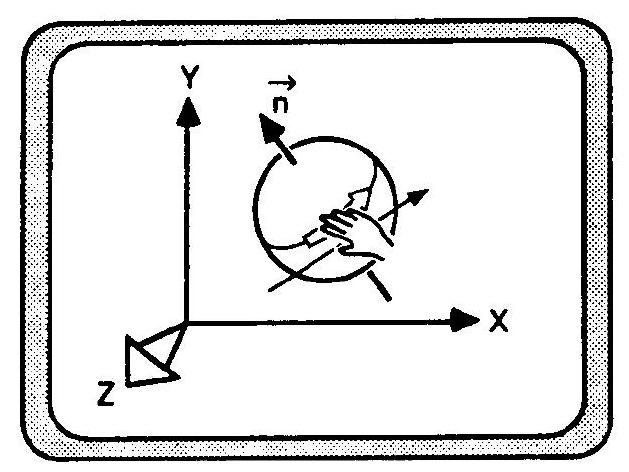
\includegraphics[max width=.35\columnwidth]{2022_11_30_0cbb01a33d99487fc27fg-084}}\hspace{5pt}
	\subfigure[前景和背景物体的合成图像。前景是“聚焦”。]{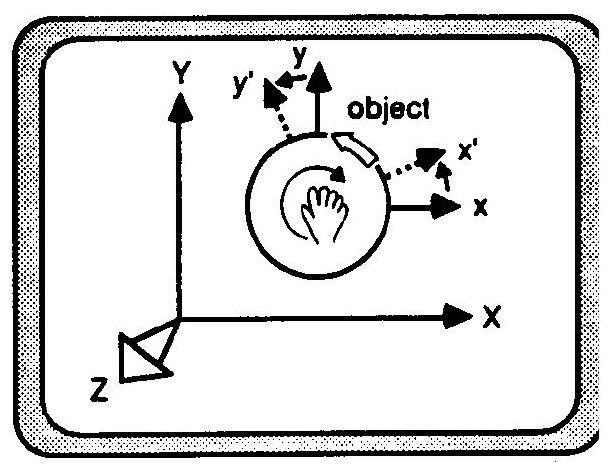
\includegraphics[width=.35\columnwidth]{2022_11_30_0cbb01a33d99487fc27fg-084(1)}}
	\caption{滚动球算法中使用的两种基本技术用于实现图形对象的任意空间旋转。a)用鼠标按黑色箭头指示的方向移动手,使物体绕位于屏幕平面上的轴$\vec{n}$旋转,即使赤道沿空心箭头方向旋转。b)小圈移动手,使物体绕屏幕平面法线旋转,方向与手的运动方向相反,再次旋转赤道沿空心箭头方向。}
\end{figure}

下面给出的滚动球算法的数学形式实际上是Chen等人(1988)在广泛调查方向控制方法中所研究的算法的一部分;我们的方法以Chen等人(1988)没有处理过的方式利用和扩展了算法的属性。滚动球应该被理解为一种新颖的、上下文无关的方法,它利用了通常以上下文相关的方式使用的已知旋转算法。


下面的处理包括两个主要部分。第一部分介绍了如何使用滚动球法进行三维定位控制,以及如何在交互式图形系统中实现它。第二部分描述了如何将滚动球方法扩展到科学可视化中极为重要的其他转换组;滚动球法被看作是一个迷人的工具,在它自己的权利可视化变换组的性质。



\subsection*{使用方法}
为了理解这个方法的基本原理,假设一个球放在桌子上,在你手掌的水平下方。


球绕任何与桌面平行的轴旋转时,都是通过手在垂直于轴的方向上水平移动,从而使球绕该轴旋转。注意,这个类的任何单一运动都不会产生围绕垂直轴的旋转,垂直于手掌的轴。


然而,如果你把你的手平放在一个球的顶部,并在水平的小圆圈中移动你的手,球实际上会绕着垂直轴向相反的方向旋转。


控制空间方向的滚动球算法是通过将要旋转的图形对象的方向作为球本身的方向来实现的,同时使用鼠标(或类似的二维输入设备)来模拟手掌的动作。


通过执行鼠标(或手)的指示动作,可以使用滚动球算法在显示的图形对象上实现以下效果:


\begin{itemize}

\item 绕水平屏幕线或$x$-轴旋转,是通过相对于查看器向前或向后移动鼠标来实现的。


\item 通过向左或向右移动鼠标,可以旋转垂直屏幕线或y轴。


\item 绕屏幕平面上的对角线旋转,我们用向量$\vec{n}$表示其方向,通过垂直移动鼠标到$\vec{n}$来实现,就像手掌在绕轴$\vec{n}$旋转圆柱或球一样。


\item 小的顺时针旋转垂直于屏幕,或z轴,通过移动鼠标在小的,逆时针的圆圈。更明显的旋转是通过使用更大的圆周运动来实现的。


\item 小的逆时针旋转,垂直于屏幕是通过移动鼠标在小的,顺时针的圆圈。


\item 围绕屏幕垂直方向的大旋转是通过向任何方向旋转对象$90^{\circ}$来实现的,围绕原始屏幕垂直轴旋转所需的量(现在位于屏幕平面上),然后旋转$90^{\circ}$来恢复原始屏幕垂直轴的方向。这个动作本质上是一个大的长方形运动,与绕屏幕垂直旋转的小圆形运动形成对比。


\end{itemize}

图1总结了两个最基本的动作,绕屏幕平面上的轴$\vec{n}$旋转和绕屏幕垂直轴旋转。


输入设备光标的位置与滚动球算法无关,在旋转操作期间,它通常对用户是不可见的。计算只需要先前和当前设备位置之间的差异,因此通常需要在每次移动后将鼠标弯曲到屏幕中央,以防止它离开交互窗口。因此,该方法是真正的上下文无关的,非常适合强调直接操作的用户界面。

\subsection*{实现}
滚动球算法是通过取一个给定的增量输入设备运动来定义一个在右屏幕坐标系中包含组件($dx, dy$)的向量来实现的。右旋轴$\vec{n}$被定义为位于屏幕平面上的垂直于输入设备运动的以下单位向量:


\begin{align}
\mathrm{n}_{\mathrm{x}}=\frac{-\mathrm{dy}}{\mathrm{dr}}, \quad \mathrm{n}_{\mathrm{y}}=\frac{+d \mathrm{x}}{\mathrm{dr}}, \quad \mathrm{n}_{\mathrm{z}}=0
\end{align}

这里我们定义了输入设备的位移$d r=\left(\mathrm{dx}^{2}+\mathrm{dy}^{2}\right)^{1 / 2}$。

其次,引入了该算法的单一自由参数——有效滚动半径$R$,它决定了旋转角度对位移$d R$的灵敏度;如果$d r$只有几个像素,那么大约100的$ r$值是合适的。我们选择旋转角度为$\theta=\arctan (\mathrm{dr} / \mathrm{R}) \approx(\mathrm{dr} / \mathrm{R})$,使

\begin{align}
\begin{aligned}
&\cos \theta=\frac{R}{\left(R^{2}+d r^{2}\right)^{1 / 2}} \\
&\sin \theta=\frac{d r}{\left(R^{2}+d r^{2}\right)^{1 / 2}}
\end{aligned}
\end{align}

绕轴$\vec{n}$旋转一个角度$\theta$的矩阵的一般形式是,其中$\vec{n} \cdot \vec{n}=1$,(参见M. Pique在Graphics Gems I, p. 446 [Glassner, 1990]中的“矩阵技术”):

\begin{align}
\left|\begin{array}{ccc}
\cos \theta+\left(n_{x}\right)^{2}(1-\cos \theta) & n_{y} n_{x}(1-\cos \theta)-n_{z} \sin \theta & n_{x} n_{z}(1-\cos \theta)+n_{y} \sin \theta \\
n_{y} n_{x}(1-\cos \theta)+n_{z} \sin \theta & \cos \theta+\left(n_{y}\right)^{2}(1-\cos \theta) & n_{y} n_{z}(1-\cos \theta)-n_{x} \sin \theta \\
n_{z} n_{x}(1-\cos \theta)-n_{y} \sin \theta & n_{z} n_{y}(1-\cos \theta)+n_{x} \sin \theta & \cos \theta+\left(n_{z}\right)^{2}(1-\cos \theta)
\end{array}\right|
\end{align}


将Eq.(2.3.1)中$\vec{n}$的值代入Eq.(2.3.3),得到滚动球旋转矩阵

\begin{align}
\left|\begin{array}{ccc}
\cos \theta+(d y / d r)^{2}(1-\cos \theta) & -(d x / d r)(d y / d r)(1-\cos \theta) & +(d x / d r) \sin \theta \\
-(d x / d r)(d y / d r)(1-\cos \theta) & \cos \theta+(d y / d r)^{2}(1-\cos \theta) & +(d y / d r) \sin \theta \\
-(d x / d r) \sin \theta & -(d y / d r) \sin \theta & \cos \theta
\end{array}\right|
\end{align}



其中三角函数的值由式(2.3.2)给出。我们观察到:

\begin{itemize}
\item 在应用式(2.3.4)之前,必须将所有向量转换到所需的旋转中心。


\item 旋转必须在一个单独的步骤中执行,如Eq.(2.3.4)。执行旋转作为一个序列,例如,首先绕$x$-轴,然后绕y轴,将给出一个完全不同的结果(尽管,由于微妙的原因,差异可能几乎是不可观察的)。


\item 更改$\vec{n}$的整体符号将产生围绕对象的视点旋转,而不是视图内的对象旋转。小的顺时针的手运动将产生小的顺时针旋转的视点,但在视图中心的对象将继续逆时针旋转。这一现象源于群理论对身体固定旋转和空间固定旋转描述的符号差异(Whittaker, 1944)。

\end{itemize}

\subsection*{滚球法的推广}
当我们分析滚动球法的群论背景时,各种相关的应用立即浮现出来。在这里,我们总结了普通旋转所涉及的基本群论,以及几个易于实现的扩展。这些技术对于许多科学可视化应用程序都很有用,包括建立关于一般群体的直觉。如果读者对群论没有兴趣,只是想知道如何实现和使用算法,就不必再读下去了。

\subsection*{无穷小旋转的群论}
涉及滚动球行为的基本群论(Edmonds, 1957)可以总结如下:如果我们定义$L_{i}, i=\{x, y, z\}$为旋转群$O$(3)的无穷小产生子,具有正旋转的右手约定,那么我们就有了对易关系

\begin{align}
\left[\mathrm{L}_y, \mathrm{L}_{\mathrm{z}}\right]=-\mathrm{L}_x, \\
\left[\mathrm{L}_z, \mathrm{L}_{\mathrm{x}}\right]=-\mathrm{L}_y, \\
\left[\mathrm{L}_x, \mathrm{L}_{\mathrm{y}}\right]=-\mathrm{L}_z,
\end{align}
其中我们使用了定义$[\mathrm{A}, \mathrm{B}]=\mathrm{AB}-\mathrm{BA}$。这些无穷小生成器可以表示为矩阵,也可以表示为这种形式的微分算子


$$
\mathrm{L}_{\mathrm{x}}=\mathrm{y} \frac{\partial}{\partial \mathrm{z}}-\mathrm{z} \frac{\partial}{\partial \mathrm{y}}
$$

和它的循环排列。方程式中的负号。(5-7)不是任意的,而是由我们的惯例决定的,$\mathrm{L}_{\mathrm{i}}$使用右手规则绕第i轴旋转一个向量。这个负号直接导致了观测到的反旋转,是旋转群性质的必然结果。


\subsection*{四元数旋转,$2 \times 2$矩阵,和SU(2)旋量}
滚动球变换用于定义四元数旋转(例如,参见Shoemake, 1985,或p - g的“使用四元数”)。Maillot在Graphics Gems I,第498页[Glassner, 1990])甚至比普通的空间旋转更自然。这是因为四元数公式等价于组SU(2)的更标准的$2 \times 2$矩阵表示法,SU(2)是通常旋转组O(3)的双重覆盖(Edmonds, 1957)。(尽管这两个基团对应完全不同的拓扑空间,但它们被滚动的球利用的无穷小性质是相同的。)


为了利用滚动球进行SU(2)转动,我们用

\begin{align}
\mathrm{U}=I_{2} \cos \frac{\theta}{2}-i\vec{n} \cdot \vec{\sigma} \sin \frac{\theta}{2},
\end{align}
其中$I_{2}$是$2 \times 2$单位矩阵,$\vec{\sigma}$表示SU(2)服从循环关系$\sigma_x^{2}=1, \sigma_x \sigma_Y=i \sigma_z$的$2 \times 2$矩阵基。这相当于一个基于四元数的转换,其中$(c, u)=(\cos (\theta / 2)$, $\vec{n} \sin (\theta / 2)$)。注意,与完整矩阵Eq.(3)相比,Eq.(8)合并滚动球的基本参数要简单得多。

更改$\vec{n}$的整体符号将产生围绕对象的视点旋转,而不是视图内的对象旋转。


矩阵Eq.(8)的元素可以根据需要从Eq.(3)中计算一个普通的矢量旋转矩阵,也可以直接用作$2 \times 2$矩阵来旋转旋量(Edmonds, 1957),这是旋转群所能作用的最基本对象。

\subsection*{欧几里得四维}
在四维欧氏空间中,0(4)群有6个转动自由度,而不是由于$0(3)$而在三维空间中存在的3个。


6个$0(4)$旋转算子$\mathrm{L}_{\mu v}, \mu, v=\{1,2,3,4\}, L_{\mu v}=-L_{\mu v}$,可以通过定义以下组合分解为$O (3) \times 0 (3)$:

\begin{align}
L_{\mathrm{i}}^{\pm}=\frac{1}{2}\left(\frac{1}{2} \epsilon_{\mathrm{ijk}} L_{\mathrm{jk}} \pm L_{4 \mathrm{i}}\right) .
\end{align}
这里$\epsilon_{i j k}$是三维中的完全反对称张量,我们使用重复罗马指标从1到3求和的惯例。每一个组合都服从独立的$0(3)$变换关系,

\begin{align}
\left[L_{1}^{\pm}, L_{\mathrm{j}}^{\pm}\right]=-\epsilon_{\mathrm{ijk}} L_{\mathrm{k}}^{\pm}, \quad\left[L_{\mathrm{i}}^{\pm}, L_{\mathrm{j}}^{\mp}\right]=0,
\end{align}
因此可以使用$O(3)$滚动球算法单独控制。以这种方式产生的旋转可以写成

\begin{align}
R^{\pm}=I_{4} \cos \theta+\vec{n} \dot \vec{L}^{\pm} \sin \theta,
\end{align}


其中

$$
\vec{n} \cdot \vec{L} \pm=\left|\begin{array}{cccc}
0 & -n_{z} & n_{y} & \mp n_{x} \\
n_{z} & 0 & -n_{x} & \mp n_{y} \\
-n_{y} & n_{x} & 0 & \mp n_{z} \\
\pm n_{x} & \pm n_{y} & \pm n_{z} & 0
\end{array}\right|,
$$
单位向量$\vec{n}$通常由式(1)定义。因此,我们可以使用滚动球的两个副本来操纵四维方向的所有自由度,一个为$\mathrm{L}_{1}^{+}$,一个为$\mathrm{L}_{\mathrm{i}}^{-}$。


另一种方法也适用于N维欧氏空间中的旋转,它是将群$O(4)$(或$\mathrm{N}$中的$O(\mathrm{~N}$))分解为$O$(3)子群,并将每个子群视为独立的滚动球变换。

\subsection*{洛伦兹变换}
研究高速物理系统必须使用时空洛伦兹变换,而不是欧几里得旋转。洛伦兹变换将空间和时间混合在一起,保留了一个具有一个负分量的闵可夫斯基空间二次型。纯粹的速度变化,或“加速”,在形式上类似于用双曲函数取代三角函数的旋转。速度$\vec{v}=\hat{} v \tanh \xi$通过矩阵转换向量$(\vec{x},t)$
\begin{align}
\left|\begin{array}{cc}
\delta_{i j}+\hat{v}_{i} \hat{v}_{j}(\cosh \xi-1) & \hat{v}_{j} \sinh \xi \\
\hat{v}_{i} \sinh \xi & \cosh \xi
\end{array}\right| .
\end{align}

为了实现$O(2,1)$洛伦兹转换(它保留了diag $(1,1,-1)$的形式),我们将鼠标运动解释为“洛伦兹滚动球”在鼠标移动方向上的微小速度变化。(我们也可以研究物理时空的变换群$0(3,1)$;不幸的是,导致式(10)的论点的类比需要引入复向量。)


$\mathrm{O}(2,1)$转换的无穷小生成器是boost操作符


$$
B_{\mathrm{x}}=t \frac{\partial}{\partial x}+x \frac{\partial}{\partial t}, \quad B_{y}=t \frac{\partial}{\partial y}+\mathrm{y} \frac{\partial}{\partial t} ,
$$
和操作符

$$
L=x \frac{\partial}{\partial y}-y \frac{\partial}{\partial x}
$$

在$x-y$面上产生旋转。boost算子在旋转下变换为普通向量,$\left[L, B_{x}\right]=-B_{y},\left[L, B_{y}\right]=+B_{x}$,而它们的相互交换产生的旋转符号与类似的$O(3)$算子,$\left[B_{x}, B_{y}\right]=+L$相反。


我们将鼠标输入与$O(2,1)$转换Eq.(12)关联起来,将Eq.(1)替换为

\begin{align}
\hat{v}_x=\frac{+dx}{dr}, \quad \hat{v}_y=\frac{+dy}{dr}
\end{align}

选择boost参数为$\xi=\tanh ^{-1}(\mathrm{dr} / \mathrm{s}) \approx(\mathrm{dr} / \mathrm{s})$,其中's是一个合适的缩放因子,确保$(\mathrm{dr} / \mathrm{s})<1$。


然后我们发现,在小的顺时针方向移动输入设备会产生顺时针方向坐标框架的空间部分的旋转,这与标准$O(3)$旋转的结果相反!这种效应被称为托马斯进动,使滚动球技术成为洛伦兹变换的一种非常自然的技术。


\subsection*{总结}
总之,滚动球技术提供了一种在交互式图形系统中使用二维输入设备控制三个转动自由度的方法,这种方法不依赖于输入设备的状态、位置或历史。由于算法丰富的群论起源,许多相关的科学可视化应用自然而然地出现了。要想熟练使用该技术,用户需要付出一些努力。但是,一旦掌握了这种方法,就会提供与情境无关的、探索性的方向调整,强烈支持直接操作的感觉。

\subsection*{鸣谢}
这项工作的一部分得到了美国国家科学基金会的资助。是- 8511751。

See also G1, 462 .\\

\newpage
\section{区间运算}
\begin{center}
\small{
Jon Rokne\\
The University of Calgary\\
Calgary, Alberta, Canada}
\end{center}


在计算机图形学中,离散化问题发生在两个不同的领域:

\begin{itemize}
\item 计算的最终输出是用有限分辨率的设备显示或打印的二维图像,这会造成诸如混叠等不良影响。


\item 确定位置、强度和颜色所需的计算在通用计算设备或专用图形计算机中进行。在任何一种情况下,存储实数的基本方法都是所谓的浮点表示。这种表示为存储浮点数分配固定数目的二进制位数,浮点数可以是输入或输出量,也可以是中间计算的结果。

\end{itemize}

我们将讨论一种工具,区间分析,它使用有保证的上界和下界来估计和控制在数值计算中可能出现的数值误差,特别是在计算机图形问题中出现的数值误差。区间算术是一门涉及面很广的学科,我们只涉及到一些基本思想。然而,我们注意到区间算术和分析已经导致了基于包含和收缩的新技术的发展,这些技术适用于计算机图形学中的一些问题。


我们首先给出一个可能发生在图形应用程序中的问题的例子。一个基本例程可能包括确定两条线(为了简单起见,在$E^{2}$中)是否平行(也就是说,它们是否有一个有限的交集)。如果它们相交,计算交点。让线条保持原样


\begin{align}
0.000100 x+1.00 y&=1.00 \\
1.00 x+1.00 y&=2.00
\end{align}
假设这个算法是一个三位数四舍五入的算法。四舍五入到五位数的真正解是$x=1.0001$和$y=0.99990$,而使用Forsythe和Moler(1967)中描述的过程,三位数的算术给出$y=1.00, x=0.00$。在本文中,使用不同的计算顺序安排也得到了其他错误的结果。从这个例子可以看出,这样的计算可能有很大的误差,以致于一个应该在区域内的交集实际上可能被计算在区域外。

另一个例子是区域填充,其中区域的连通性依赖于一个计算,该计算可能以与交叉计算相同的方式充满错误。

这样的错误很难防范,最终它们会在计算机生成的场景中产生不受欢迎的工件,并且很难在大型程序中跟踪和纠正。

其中许多误差可以使用区间算法自动控制。它使程序能够给出项目$p$和集合$P$的三个答案之一。


\begin{enumerate}
	\item $p$肯定在$P$中。


\item $p$肯定不在$P$中。


\item 在执行的计算和可用的精度中,不可能告诉$p \in P $或$p \notin P $,也就是说,结果是不确定的。
\end{enumerate}

根据前面的例子,我们可以说直线相交,它们不相交,或者它们是否相交是不确定的。类似地,我们可以声明一个域是连接的,它是没有连接的,或者域是否连接是不确定的。在每一种情况下,可以将决策程序内置于程序中以处理这三种情况。


区间运算有着悠久的历史;然而,它的现代使用源于摩尔(1966)的《区间分析》一书的出版。后来,有大量的出版物专门讨论这个问题。Garloff出版了参考书目(1985,1987),举行了一些会议,最近出版了一份新的苏联期刊,《区间计算》(新技术研究所,1991),完全致力于区间分析。

区间算术定义如下:设 $I=\{A: A=[a, b], a \cdot b$ $\in \mathrm{R}\}$为实紧区间集,设$A, B \in I$。然后区间算术运算定义为

$$
\mathrm{A} * \mathrm{~B}=\{\alpha * \beta: \alpha \in \mathrm{A}, \beta \in \mathrm{B}\} \text {, }
$$
其中 $* \in\{+,-, \cdot, /\}$(注意 / 在 $0 \in B$ 时未定义),即 $A * B$ 的区间结果包含所有可能的点结果 $\alpha * \beta$,其中 $\alpha$ 和 $\beta$ 是实数,使得 $\alpha \in A$ 和 $b\eta in B$ 和 $*$ 是基本的算术运算之一。

这个定义是由下面的论证驱动的。给定两个区间$A$和$B$,我们知道它们分别包含精确的值$x$和$y$。然后定义保证$x * y \in A * B$中用于上述任何操作,即使我们不知道$x$和$y$的确切值。

这个定义在实际计算中不是很方便。令$A=[a, b]$,且$ B=[c, d]$,可得其等价于

\begin{align}
\begin{aligned}
{[a, b]+[c, d] } &=[a+c, b+d], \\
{[a, b]-[c, d] } &=[a-d, b-c], \\
{[a, b] \cdot[c, d] } &=[\min (a c, a d, b c, b d), \max (a c, a d, b c, b d)], \\
{[a, b] /[c, d] } &=[a, b][1 / d, 1 / c] \text { if } 0 \sim[c, d],
\end{aligned}
\end{align}

这意味着在$* \in\{+,-, \cdot, /\}$中的每个区间操作都被简化为真正的操作和比较。


区间算术的一个重要性质是


\begin{align}
\begin{aligned}
A, B, C, D \in A \subseteq B, C \subseteq D, \Rightarrow A_{\sqcup} * C C_{\sqcup} \subseteq B_{\sqcup} & * D \\
& \text { for } * \in\{+,-, \cdot, /\}
\end{aligned}
\end{align}

如果定义了操作。换句话说,如果$A$和$C$分别是$B$和$D$的子集,那么$A * C$是用于任何基本算术操作的$B * D$的子集。因此,在计算的任何阶段引入的错误,如浮点错误或输入错误,都可以被解释。由于式(4)的重要性,它被称为区间运算的包含等度。

如果定义了操作。换句话说,如果$A$和$C$分别是$B$和$D$的子集,那么$A * C$是用于任何基本算术操作的$B * D$的子集。因此,在计算的任何阶段引入的错误,如浮点错误或输入错误,都可以被解释。由于式(4)的重要性,它被称为区间运算的包含等度。

这样做的一个结果是,任何可编程的实计算都可以使用操作之间的自然对应关系嵌入到区间计算中,因此,如果$x \in X \in I$中,则$f(x) \in f(X)$中,其中$f(X)$被解释为$f(. x)$ , $x$替换为$X$,操作替换为区间操作。

间隔算术的另一个重要原理是,它可以在浮点计算机上实现,这样得到的间隔包含使用等式进行的真实间隔计算的结果。(3)和定向四舍五入。有几种软件系统可用于此目的,如PASCAL-SC (Bohlender et al., 1981)。实现只需要注意间隔端点的每个计算都是从间隔的内部向外舍入。

区间算术也有一些缺点:


\begin{itemize}
\item 减法和除法不是加法和乘法的逆运算。

\item 分配律不成立。只有子分配律$\mathrm{a}(\mathrm{B}+$ C) $\subseteq \mathrm{AB}+\mathrm{AC}, \mathrm{a}, \mathrm{B}, \mathrm{C} \in\mathrm{I}$是有效的。

\item 区间算术操作比相应的实际操作大约耗时3倍(尽管某些问题的区间算术实现可能比相应的实际版本运行得更快;参见suffn and Fackerell, 1991)。
	


\end{itemize}

作为使用区间计算的一个简单例子,我们使用三位区间算术来考虑上面给出的相交线问题。根据克拉默法则,我们得到


$$
\mathrm{x}=\left|\begin{array}{cc}
1.00 & 0.000100 \\
2.00 & 1.00
\end{array}\right| /\left|\begin{array}{cc}
0.000100 & 1.00 \\
1.00 & 1.00
\end{array}\right|
$$
和
$$
\mathrm{y}=\left| \begin{array}{cc}
0.000100 & 1.00 \\
1.00 & 2.00
\end{array}\right| / \left|\begin{array}{cc}
0.000100 & 1.00 \\
1.00 & 1.00
\end{array}\right|.
$$
利用区间算法得到
$$
\mathrm{x} \in \mathrm{X}=[0.980,1.03]
$$
和
$$
\mathrm{y} \in \mathrm{Y}=[0.989,1.02],
$$
在每种情况下都包含精确解。这个计算与Forsythe和Moler(1967)引用的计算相比,在实际算术中对应更稳定的计算。如果这个特定的计算序列是在区间算术中执行的,那么间隔会更大,但在所有情况下,准确的结果都包含在结果的区间中。

区间算术的一个有趣的特点是,它可以用来开发新的算法,而不是简单地扩展实际算术中的算法。其中一个例子是摩尔(1966)首先提出的区间牛顿法。假设给定$\mathrm{F}(\mathrm{x})$,并假设我们想要找到在给定区间$X_{0}$中$F(\xi)=0$的点$\xi$。然后定义区间牛顿法为迭代

$$
\mathrm{X}_{\mathrm{n}+1}=\mathrm{m}\left(\mathrm{X}_{\mathrm{n}}\right)-\mathrm{F}\left(\mathrm{X}_{\mathrm{n}}\right) / F^{\prime}\left(\mathrm{m}\left(\mathrm{X}_{\mathrm{n}}\right)\right), \quad \mathrm{n}=0,1, \ldots,
$$
其中$m([a ; b])=\left((a+b) / 2\right.$和$F^{\prime}(X)$是$F$的导数的区间求值。这个方法有一些有趣的性质。

\begin{enumerate}
\item 如果$F$的0 $\xi$存在于$X_{0^{\prime}}$中,则对于所有$n$, $\xi \in X_{n}$中;见Moore(1966)。这意味着初始$X_{0}$中的所有零都保留在后续的间隔中。

\item 如果$X_{n^{\prime}}$对于某个$n$是空的,那么$F$在$X$中没有零(Moore, 1966)。

\end{enumerate}

方程解的区间迭代的进一步性质可以在neuaier(1990)中找到。

该方法可应用于计算机图形学中的射线跟踪。隐式曲面和射线之间的交点计算会导致一个问题,即找到函数$\mathrm{F}(\mathrm{x})=0$的一个(最小)根或所有根(见Hanrahan, 1989)。通过使用区间算术技术,可以保证结果包含在生成的区间中,避免渲染过程中的异常(参见Kalra和Barr, 1989,关于该问题的讨论)。

在Mudur和Koparkar(1984)以及summern和Fackerell(1991)中,我们发现了在隐式表面绘制中使用区间算法,在轮廓绘制算法和面度估计中使用区间算法的进一步讨论,其中它与细分技术相结合,以改善结果。

See also G2, 394.


\newpage
\section{快速生成循环序列}
\begin{center}
\small{
Alan W. Paeth\\
NeuralWare Incorporated\\
Pittsburgh, Pennsylvania}
\end{center}

自由运行的内部循环通常需要一系列重复每个$N$步骤的值或条件。例如,高速z -缓冲区绘制技术(Booth et al., 1986)必须以三个周期执行缓冲区交换和内务管理。当$N$不是2的幂时,直接检查寄存器的低阶位可能不会被用来形成N的计数模。类似地,一个快速的二维N-gon生成器需要循环生成$N$的值序列,顶点$N$与顶点0相同。这个Gem考虑了$N<8$的紧凑方法,它使用的机器指令不超过三条,也不超过三个寄存器。不使用条件逻辑,使得该技术非常适合手工编码。

Free-running inner-loops often require a sequence of values or conditions that repeat every $\mathrm{N}$ steps. For instance, a technique for high-speed Z-buffer drawing (Booth et al., 1986) must perform buffer swapping and housekeeping in cycles of three. When $\mathrm{N}$ is not a power of two, direct examination of a register's low order bits may not be used to form a count modulo N. Similarly, a fast 2-D N-gon generator requires the cyclic production of a sequence of $\mathrm{N}$ values, with vertex $\mathrm{N}$ identical to vertex zero. This Gem considers compact methods for $\mathrm{N}<8$ that use neither more than three machine instructions nor three registers. No conditional logic is employed, making the techniques well-suited to hand coding.

\subsection*{$N=2$ (Review)}
我们熟悉的双重“toggle”在true和false之间交替:


\begin{align}
\begin{aligned}
&\text { condition := not(condition); } \quad \textit { True in alternating cases } \\
&\text { if (condition) } . . .
\end{aligned}
\end{align}


Similarly, a two-fold "cycle" of values is a simple alternation. When both values are predeterminated, one instruction and one integer register suffice:

$$
\begin{array}{ll}
\text { register } a:=v 1 ; & \text { initialize } \\
\text { constant } c:=v 1+v 2 ; & \\
\text { repeat } & \text { cycle } \\
%\quad a:=a-c ; & a:[v 1 \text { v2ن } \cdots]
\quad a:=a-c ; & a:[v 1 \text { v2} \cdots]
\end{array}
$$

For instance, Wirth (1973) speeds a prime number sieve by using (2.2) to generate the sequence $\left[\begin{array}{lllll}2 & 4 & 2 & 4 & \cdots\end{array}\right]$ of distances between successive odd integers not divisible by three (Knuth, 1981). Rewriting the arithmetic of (2.2) with logical xor operations yields a well-known, patented method for inverting a frame-buffer's pixels in alternating fashion. In arithmetic form, a pixel inversion scheme well-suited to greyscale frame buffers is rederived (Newman and Sproull, 1979).

Most generally, the cyclic sequence is specified only at run time. For $\mathrm{N}=2$, cycling is swapping, easily accomplished in three arithmetic or logical operations without resort to a third holding register, as described in previous Gems by Paeth (1990) and Wyvill (1990), respectively.

\subsection*{$N=3$ (Extension)}
The pairwise swapping technique does not extend gracefully: Cyclic permutation of the sequence [a, b, c] by exchanging (for example) elements at locations $(1,2)$ and $(2,3)$ costs six instructions and three registers. A first-principles cyclic brigade method requires $\mathrm{N}+1$ registers and $\mathrm{N}+1$ assignments. Though straightforward, the latter still exceeds both the instruction and register limits set forth in the preface:

$$
\begin{aligned}
& \text { r1 :=r1 xor r2; } \quad \text { r2 :=r2 xor r1; } \quad \text { rx }:=r 1 ; \quad r 1:=r 2 \text {; } \\
& \text { r1 :=r1 xor r2; } \quad \text { r2:=r2 xor r3; <versus> } \quad r 2:=r 3 ; \quad r 3:=r x ; \\
& \text { r3 }:=\text { r3 xor r2; } \quad \text { r2 }:=\text { r2 xor r3 }
\end{aligned}
$$

Often, as in (2.1), values are required only to trigger a 1-in-N event. For $\mathrm{N}=3$, two registers and two lines suffice. Each register instruction is of the compact, two-op form $\ll r x=r x$ op ry $\gg$ :

$$
\begin{aligned}
& \text { register r1 }:=0 ; \quad \text { Three fold trigger } \\
& \text { register r2 :=1; } \\
& \text { repeat cycle: }
\end{aligned}
$$

This produces the tertiary (r1, r2) column set shown. The trigger occurs when a register is zero. Testing on r2 streamlines the operation under the

\begin{center}
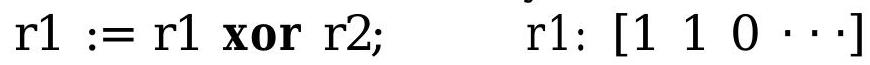
\includegraphics[max width=\textwidth]{2022_11_30_0cbb01a33d99487fc27fg-100}
\end{center}

\begin{center}
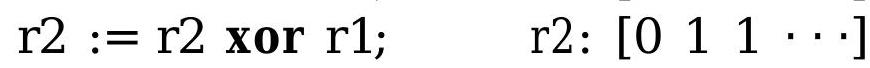
\includegraphics[max width=\textwidth]{2022_11_30_0cbb01a33d99487fc27fg-100(1)}
\end{center}

\section{II.5 FAST GENERATION OF CYCLIC SEQUENCES}
assumption that hardware condition codes are set by the preceeding logical operations. The phase of the test may be adjusted by substituting a column other than the third in the initialization of ( $\mathrm{r} 1, \mathrm{r} 2)$. Triggering 2-in-3 times defines the complementary set: a test for nonzero is substituted. The three phase-distinct 1-in-3 tests may be done concurrently, forming a cyclic switch:

$$
\begin{array}{ll}
\text { if } r=0 \text { then } \cdots & 1 \text {-in-3, phase }=0 \\
\text { if } r l=r 2 \text { then } \cdots & 1 \text {-in-3, phase }=1 \\
\text { if } r l=0 \text { then } \cdots & 1 \text {-in-3, phase }=2
\end{array}
$$

The conditions and related blocks may be embedded among the xor operations to take advantage of implicit condition code sensing. That is, the two xor lines that implicitly define the modulo three counter need not be adjacent.

Cyclic permutation of three variables in three registers can be done in the minimum number of instructions (three). The derivation is not obvious and relates the threefold arithmetic case described later.

$$
\begin{aligned}
&\text { register int } a=c 1 ; \quad \text { Three fold cycle } \\
&\text { register int } b=c 1 \text { xor } c 2 \text {; } \\
&\text { constant int } c=c 1 \text { xor } c 2 \text { xor } c 3 \text {; }
\end{aligned}
$$

$$
\begin{aligned}
& \text { repeat cycle: } \\
& \mathrm{a}=\mathrm{a} \text { xor } \mathrm{b} \text {; } \\
& \text { a: [c1 c2 c3...] } \\
& \mathrm{b}=\mathrm{b} \text { xor } \mathrm{c} \text {; } \\
& \mathrm{b}=\mathrm{b} \text { xor } \mathrm{a} \text {; }
\end{aligned}
$$

The use of logical xor is valuable as the elements may be a mixed sequence of integers, pointers and floats; arithmetic operations would not permit this. Note that the last two lines both update the value in b, while register c is never written. This suggests the alternate line:

$$
\mathrm{b}:=\mathrm{b} \text { xor (a xor } \mathrm{c} \text { ) }
$$

in which $\mathrm{c}$ is equated to a predetermined compile time constant. However, the value must typically occupy a third register at run time. (See the C-code for a two register variant which produces the cycle [1, 2, 3].)


When mere triggering is required, fixing $\mathrm{c}=0$ elides the middle line of the cycle, reconstructing the $\mathrm{N}=3$ triggering case. Alternately, the two lines may be regarded as the first two of three lines of the familiar xor swap code. Because the final line of the latter matches the first, three passes through the two-line xor code produce the same sequential action on the two registers as do two passes through the three-line code (this is suggested in Eq.(3.1a) by the grouping of instructions). Both define a restoring double swap: the identity operation on two elements in no less than six steps. Thus, the two-line code forms cycles of length three while generating the sequence $[\mathrm{r} 1, \mathrm{r} 1 \oplus \mathrm{r} 2, \mathrm{r} 2]$.

\subsection*{$N=3,4,6$}

Remarkably, cycles of length up to $\mathrm{N}_{\overline{5}} 6$ require only two registers. Clearly, there is insufficient storage for swapping of all elements, else a cyclic brigade of $\mathrm{N}+1$ registers and $\mathrm{N}+1$ assignments would suffice. Instead, the goal is to derive a set of values (on one or both registers) in which all generated values are distinct. Thus, the registers must "count," and rival first-principles code such as a quick hexagon-drawing routine:

\section{Xval =X\_ Value\_ Table[(i := (i $+1 \bmod 6))]$; 
 Yval = Y\_ Value\_ Table[i];}
Here the modulus is a major expense: its cost is on par with integer division. The other first-principles method uses conditional logic to restart a decrementing counter, giving a large branch penalty on modern pipelined hardware, made worse by small N.

As will be seen in (6.2), vertex production of 2-D hexagons may use this sixfold cycle:

$$
\begin{aligned}
&\text { register } \mathrm{x}=\mathrm{y}=1 \text {; } \\
&\text { repeat }
\end{aligned}
$$

Xval = X\_coord $[\mathrm{x}:=\mathrm{x}+\mathrm{y}] ;$

Yval = Y\_coord[y := $\mathrm{y}+\operatorname{not}(\mathrm{x})]$

where $\operatorname{not}(\mathrm{x})$ is bit inversion, i.e., $\operatorname{not}(\mathrm{x})=\mathrm{x}$ xor $(-1)$ under two

complement hardware. Arrays of length seven are required having suitable offsets, as seen in the companion C code.

\subsection*{$N=\mathbf{6}$ Derivation}
Nonuniform rotation may be modeled by functional composition. That is, $\mathrm{F}(\mathrm{F}$. . . $(\mathrm{F}([\mathrm{x}]))$. .. $)=[\mathrm{x}]$ in no less than $\mathrm{N}$ steps. For instance, the linear fractional function $F\left(x_{5}\right)_{\sqcup}\left[2 x_{\sqcup} l\right] /[x+1]$ yields $F^{6}(x)=x$ (Yale, 1975). Such forms may be equated directly to the algebra of $2 \times 2$ matrices (Birkhoff and MacLane, 1965); the former are treated preferentially for ease of derivation.

The values of two registers may be represented by a point $[x, y]$ on an integer lattice, one coordinate per register. Treated as a (column) vector $\mathrm{v}$, the function $\mathrm{F}$ is a $2 \times 2$ matrix of which premultiplies $\mathrm{v}$. For a given $\mathrm{N}$, F must be determined such that $\mathrm{F}^{\mathrm{N}} \mathrm{v}=\mathrm{I}$. When $\mathrm{F}$ is a shear matrix rotation may be achieved in three shears (Paeth, 1986), requiring only one assignment statement per shear (p.182). When the off-diagonal matrix element is $\{\pm 1\}$, no multiplication occurs and one machine instruction suffices. All-rational forms also yield rotation, but the sets of circumferential points are not roots of unity (vertices of an $\mathrm{N}$-gon inscribed in a unit circle on the complex Cartesian plane). The one solution is for fourfold rotation. That decomposition is:

$$
\begin{array}{cc}
0 & -1 \\
1 & 0
\end{array}=\begin{array}{cccccc}
1 & 1 & 1 & 0 & 1 & 1 \\
0 & 1 & -1 & 1 & 0 & 1
\end{array} .
$$

Regrouping of the first and third matrix (p.192) allows a two-line rotation, useful on machines that provide an implicit multiplication by two:

$$
\begin{aligned}
& \mathrm{x}:=\mathrm{x}+\mathrm{y} ; \quad \mathrm{x}:=\mathrm{x}+\left(2^{*} \mathrm{y}\right) ; \\
& \mathrm{y}:=\mathrm{y}-\mathrm{x} ; \quad<0 \mathrm{x}>\quad \mathrm{y}:=\mathrm{y}=\mathrm{x} ; \\
& \mathrm{x}:=\mathrm{x}+\mathrm{y} \text {; }
\end{aligned}
$$

This sequential form is slightly more expensive than the compact $\{x=$ $\left.-y, y_{\bar{E}} \mathrm{x}\right\}$ form made possible when simultaneous reassignment of register values is possible, as in hardware. Rotations of three and six may

be formed by finding the eigenvalues of the product of an $\mathrm{X}$ and $\mathrm{Y}$ shear in symbolic form and equating them with the roots of unity, thus determining the values of the two off-axis elements. In its most compact form, this yields the quadratic equation $z=\frac{1}{2}\left(m \pm \sqrt{m^{2}-4}\right)$, which can represent roots of unity $z^{N}=1$ for $N=\{1,2,3,4,6\}$, with the respective values $m=\{2,-2,-1,0,1\}$. Solution using MAPLE on the matrix equation $(\mathrm{XY})^{\mathrm{N}}=\mathrm{I}$ with symbolic matrix elements does not reveal real-valued, integral forms markedly distinct from this general solution:

$$
\begin{aligned}
& (\mathrm{m}, \mathrm{N})=\{(-1,3),(0,4),(1,6)\}
\end{aligned}
$$

Both three-and sixfold rotation using unit elements are thus possible. These are unexpected, given the irrationality of $\cos 60^{\circ}$. The distortion of the simplified two-shear rotational form has become a virtue in fixing vertices to integral locations. Note that the three nontrivial solutions for $\mathrm{N}=(3,4,6\}$ enumerate the set of $\mathrm{N}$-gons that tile the plane (Figs. 1a, 1b).

An automated examination of all three-instruction, three-register shears having small multipliers was conducted. No solutions for new $\mathrm{N}$ were found, and most forms were not markedly distinct. The two-register\\
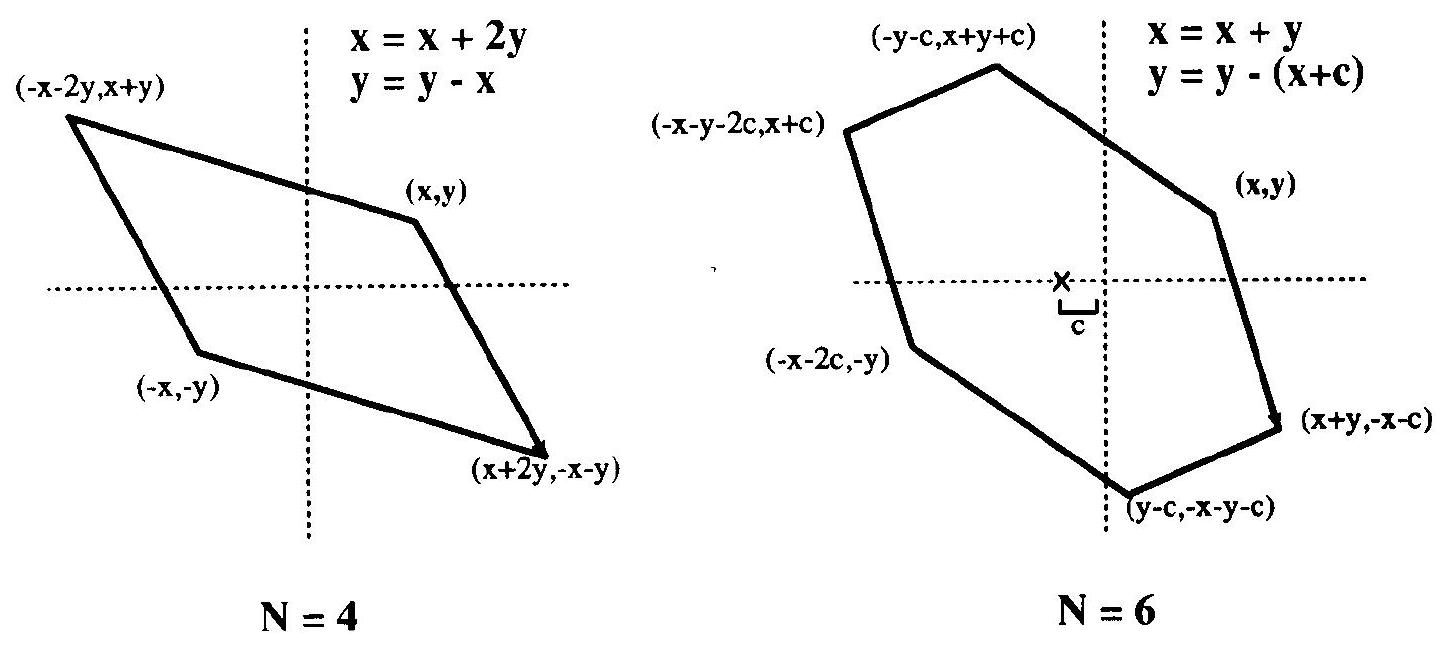
\includegraphics[max width=\textwidth, center]{2022_11_30_0cbb01a33d99487fc27fg-104}

Figure 1.

\begin{center}
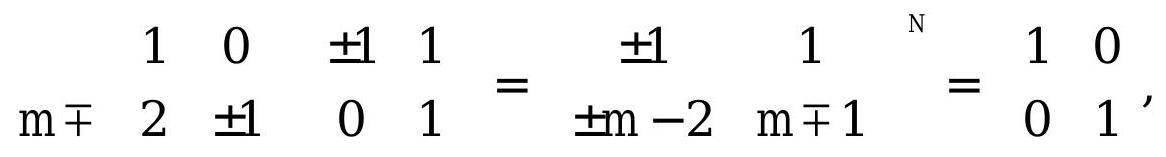
\includegraphics[max width=\textwidth]{2022_11_30_0cbb01a33d99487fc27fg-104(1)}
\end{center}

$\mathrm{N}=3$ form was rewritten using xor, leading to (3.3). The $\mathrm{N}=6$ two-register form was seen to accommodate one additional constant, which offsets the hexagon in $x$, illustrated in Fig. $1 b$ and presented algebraically below:

When $\mathrm{c}=0$, the values in register a lag those in b by two steps, suggestive of a (cos $t, \sin t)$ generator, except the $90^{\circ}$ quadrature becomes a $120^{\circ}$ phase offset. With $c \neq 0$ the generation of a sequence of distinct values is achieved, meeting the original goal. Setting $\mathrm{c}=-1$ allows the implicit formation of the - $(\mathrm{a}+1)$ term using the logical ones complement (Paeth and Schilling, 1991), giving:

$$
\begin{aligned}
& \mathrm{a}_{\bar{\Xi}}=\mathrm{b}_{\mathrm{s}}=1 ; \quad \text { six-fold fixed-ualue cycle } \\
& \text { repeat } \\
& \mathrm{a}:=\mathrm{a}+\mathrm{b} ; \quad \mathrm{a}:\left[\begin{array}{llllll}1 & 2 & 0 & -3 & -4 & -2\end{array}\right]
\end{aligned}
$$

in which the c offset displaces the hexagon's center laterally, removing symmetry of central inversion. This helps achieve distinct values. With $\mathrm{a}>0, \mathrm{~b}>0$ and $2 \mathrm{c}>\mathrm{a}+\mathrm{b}$, the sequence in $\mathrm{a}$ is always positive.

\subsection*{$\mathrm{N}=6$ (Triggering)}
Arbitrary triggering is possible using the sixfold form. The distinct values of the preceding algorithm allow concurrent 1-in- $\mathrm{N}$ triggers having any phase offset. However, 2-in-N and 3-in- $\mathrm{N}$ forms with nonadjacent triggers present greater difficulty: They may not be created by replacing equality test with an inequality. This is a consequence of the figures' convexity: In geometric terms, a test such as y $>4$ represents a horizontal half-space of values. Intersection of the polygon by the plane splits it into two distinct boundary sets of conterminous vertices. The goal is a simple trigger that does not resort to intra-register bit testing as in the companion Gem cited above.

Six states allow 64 trigger patterns, in which a "*" (".") in the ith place represents a (dis)arming of the trigger for the ith state. Elimination

\begin{center}
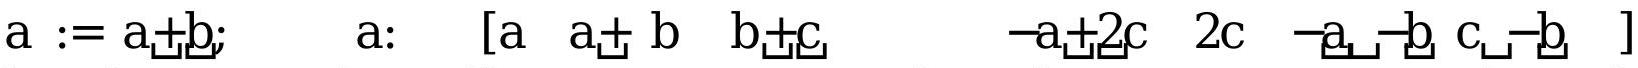
\includegraphics[max width=\textwidth]{2022_11_30_0cbb01a33d99487fc27fg-105}
\end{center}

\begin{center}
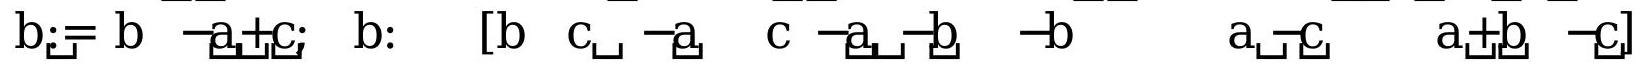
\includegraphics[max width=\textwidth]{2022_11_30_0cbb01a33d99487fc27fg-105(1)}
\end{center}

\begin{center}
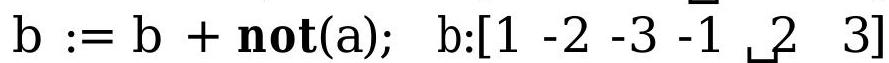
\includegraphics[max width=\textwidth]{2022_11_30_0cbb01a33d99487fc27fg-105(2)}
\end{center}

\section{II.5 FAST GENERATION OF CYCLIC SEQUENCES}
of complementary patterns halves this number. Patterns containing repetitive triggers such as “**\textit{.." and “}...." may be decomposed into super or subcycles and are eliminated. Left are three prototypical patterns, having one, two, or three bits set. Testing uses the sixfold rotation variant in (6.2) with implicit $(c=-1)$ and starting values $a=b=0$ :

$$
\begin{array}{rlrrrrrr}
\text { a: } & 0 & 0 & -1 & -2 & -2 & -1 \\
\text { b: } & 0 & -1 & -1 & 0 & +1 & +1 \\
\mathrm{a}=0 \text { AND b}= & 0: & * & \cdot & . & . & - & . \\
\mathrm{a}= & 0: & * & . & * & . & . \\
\mathrm{a}=0 \text { OR } \mathrm{b}= & 0: & * & * & . & * & .
\end{array}
$$

The widespread use of xor suggests methods similar to pseudo-random number (RPN) generation on the field of integers $\bmod 1$ (see Morton, 1990). The traditional shift and carry-test logic hardware may be "wired" directly into three xor register instructions having a permuting form, giving

$$
\begin{aligned}
& \text { repeat } \\
& \mathrm{b}:=\mathrm{b} \text { xor } \mathrm{a} \text {; } \\
& \mathrm{c}:=\mathrm{c} \text { Xorb; } \\
%& \mathrm{a}:=\mathrm{a}_{\mathbf{प}} \text { रr } \text {; }
& \mathrm{a}:=\mathrm{a}_{\mathbf{q}} 
\end{aligned}
$$

This yields the table of values listed below.

\begin{center}
\begin{tabular}{lll}
\hline
$\mathrm{A}$ & $\mathrm{B}$ & $\mathrm{C}$ \\
\hline
$\mathrm{a}$ & $\mathrm{b}$ & $\mathrm{c}$ \\
$\mathrm{a} \oplus \mathrm{b}$ & $\mathrm{b} \oplus \mathrm{c}$ & $\mathrm{a} \oplus \mathrm{b} \oplus \mathrm{c}$ \\
$\mathrm{a} \oplus \mathrm{c}$ & $\mathrm{a}$ & $\mathrm{b}$ \\
$\mathrm{c}$ & $\mathrm{a} \oplus \mathrm{b}$ & $\mathrm{b} \oplus \mathrm{c}$ \\
$\mathrm{a} \oplus \mathrm{b} \oplus \mathrm{C}$ & $\mathrm{a} \oplus \mathrm{c}$ & $\mathrm{a}$ \\
$\mathrm{b}$ & $\mathrm{c}$ & $\mathrm{a} \oplus \mathrm{b}$ \\
$\mathrm{b} \oplus \mathrm{c}$ & $\mathrm{a} \oplus \mathrm{b} \oplus \mathrm{C}$ & $\mathrm{a} \oplus \mathrm{c}$ \\
\hline
\end{tabular}
\end{center}

Here column A leads B by two steps, likewise $B$ ahead of $C$, but $C$ leads A by three steps. Each column takes on all $\mathrm{N}_{5}-1$ possible arrangements of xor among the three variables, omitting the forbidden zero state. This does not restrict the periodic production of zero elements, formed either by setting any (but not all) of $\{a, b, c\}$ to zero, or by equating initial values in two registers, since $\mathrm{M}$ xor $\mathrm{M}=0$.

Use of four registers $(r=4)$ suggests $2^{4}-1=15$ states. Since $r$ is even, $\mathrm{N}$ is composite with factors $\left(2^{2}+1\right)\left(2^{2} 2_{\sqcup}-1\right)$. This reveals the subcycle for $\mathrm{N}_{5}=5$, rounding out the table for small $\mathrm{N}$. However, this method shows only a marginal gain over the brigade method (five variables, one temporary register, six assignments) and was not explored. For those inclined to large $\mathrm{N}$, factors may be used to compose larger cycles: concurrent loops of relatively prime length resynchronize after a number of steps equal to the product (the GCM) of their lengths.

For the last single-digit value, $\mathrm{N}=9$ remains difficult as it is neither prime nor a square-free composite. The next primes at $(11,13)$ are not of the $2^{\mathrm{m}}-1$ Mersenne form. By Fermat's theorem, they (and any prime p) are factors of $2^{p-1}$, here $2^{10}{ }^{1} 1$ and $2^{12}$. 1 . Since this implies that the number of registers grows at least linearly with the cycle length for xor methods, the brigade method wins by virtue of simplicity. Although the practical limit of all methods explored thus far is $\mathrm{N}<8$, more exotic and convoluted methods are possible and may be examined through brute-force means. One is presented below.

\subsection*{$
N=24
$}

As a last example, the code

$$
\begin{aligned}
&\text { register } a=4 ; \\
&\text { register } b=3 ; \\
&\text { repeat }
\end{aligned}
$$

$\mathrm{a}:=\mathrm{a}-\mathrm{b}$

a := a bit-and 15; explicit limit on register a

$\mathrm{b}:=\mathrm{b}$ xor $\mathrm{a} ;$

offers a method of cycling modulo 24. Limiting the domain of register $a$ to 16 values necessarily introduces value multiplicity. The initial values

chosen confine both $a$ and $b$ to the domain [1..15] and further insures that they are never simultaneously equal.

This code's value is in forming parallel 24:1, 12:1, 8:1, and 6:1 rate division using the conditional tests $(b=1),(a=4),(b=7)$ and $(b=12)$, respectively. These tests are chosen so at most one is true at any step, allowing rate multiplication (up to 10-in-24) by combining the $\{1,2,3,4\}$ -in-24 tests by oring of the triggering bits. Note that only the 3-in-24 rate shows slight nonuniformity:

a: $\begin{array}{llllllllllllllll}115 & 2 & 3 & 712 & 5 & 3 & 215 & 3 & 4 & 9 & 7 & 211151213 & 112 & 7 & 11 & 4\end{array}$

\begin{center}
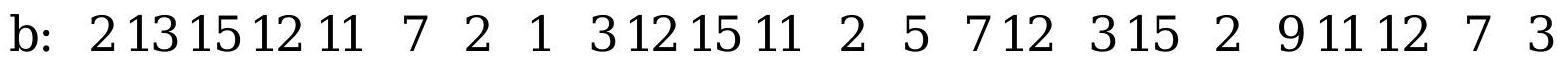
\includegraphics[max width=\textwidth]{2022_11_30_0cbb01a33d99487fc27fg-108}
\end{center}

%$\mathrm{b}_{\text {जiு }} 1: \quad *$
$\mathrm{b}_{\text {w}} 1: \quad *$
$\mathrm{a}=4:$

$\mathrm{b}_{\bar{y}=7} 7$

$\mathrm{b}_{\mathrm{y}=12:}$

\begin{itemize}
  \item 
\end{itemize}

$*$

$\$$

$x$

$k$

$*$

\subsection*{Summary}
Methods for cyclic production of both arbitrary values and of Boolean states has been presented. Cases $\mathrm{N}=\{2,3,4,6,7\}$ were treated in detail. The extensive C-code variants provided in the appendices make a useful set of additions to the graphics programmer's bag of tricks.

See also G1, 436.

\begin{center}
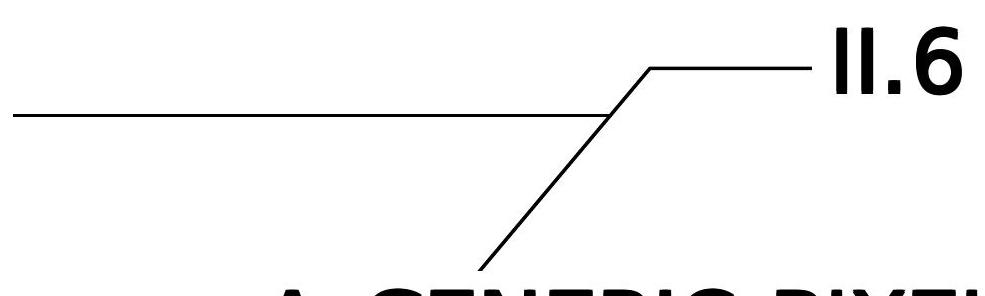
\includegraphics[max width=\textwidth]{2022_11_30_0cbb01a33d99487fc27fg-109}
\end{center}

\section*{A GENERIC PIXEL SELECTION }
 MECHANISM\begin{center}
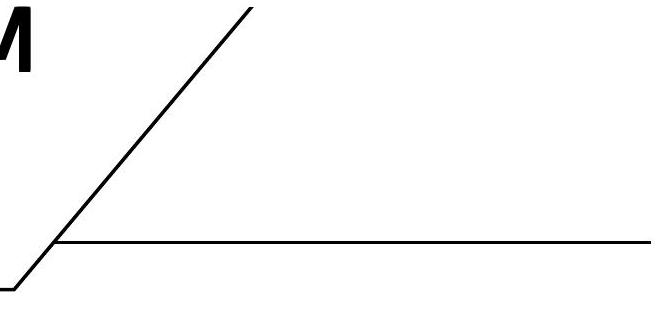
\includegraphics[max width=\textwidth]{2022_11_30_0cbb01a33d99487fc27fg-109(1)}
\end{center}

Reversing the colors of a frame buffer's pixels is a common way to highlight a region. A useful reversal function provides color pairs that are visually distinct. On newer hardware, lookup tables (which map a pixel's appearance) are keyed by window, introducing spatial dependence. This burdens the design of a "best" function. This gem offers a simple a priori solution that guarantees visually distinct color pairs, though their eventual appearance remains unknown to the algorithm. Typical use is in creating screen-wide, window-invariant tools, such as system cursors or selection rectangles for display "snapshots."

A useful reversing function $F$ on pixel $p$ satisfies two algebraic criteria: $F(F(p))=p$ and $F(p) \mu$ p. The first assures that the function is its own inverse. The second is crucial in guaranteeing that the two elements in any color pair are "not nearly equal," leaving them visually distinct. For one-bit pixels, complementation (bit toggle) is the obvious solution. At higher precision, the (ones) complement of all bits becomes an arithmetic operation: $F(p)=\operatorname{not}(p)=-1-p$ under two's complement arithmetic (Paeth, 1991). This has been generalized (Newman and Sproull, 1979) for $0 \leq c<1$ as $F_{c}(p)=\operatorname{frac}(c-p)$. This fails the second criterion: For parameter c a pixel of value c/ 2 maps onto itself. Geometrically, the unit interval has been displayed (by c) and mirrored onto the original interval, thereby introducing a stationary point.

The solution used in the Palette system (Higgins and Booth, 1986) returns to logical operations. Given a binary integer that defines discrete positions along an interval, bit complementation of merely the uppermost bit swaps the interval's lower and upper halves without any mirroring. The pixels in any color pair are now displaced by half the interval

\section{II.6 A GENERIC PIXEL SELECTION MECHANISM}
distance, guaranteeing distinct colors. In the case of color-mapped pixels (which serve as indices), elements in a pair are far removed in the domain of the mapping function, yielding colors likewise removed in the range should the color map define a monotonic function-a common case. Certain nonlinear non-Cartesian color maps (Paeth, 1991) also work well under this function and support a simple geometric interpretation.

The generic function may now be constructed by making simple assumptions. The pixel precisions of monochromatic channels on typical framebuffers are one, four, or eight bits. The operation

$$
\text { macro bwpixflip }(\mathrm{x}) \quad \mathrm{x}:=\mathrm{x} \text { bit-xor } 133 \text { hex } 85
$$

complements the topmost bit in all cases without knowledge of the precision in use. When the underlying pixel is of lower precision, toggling the higher-order bits is of no consequence or is squelched by action of a hardware write mask. Conversely, operation upon a high precision, pixel will complement additional low-precision bits, but these are sufficiently removed to be of much consequence.

For RGB pixels, three copies of hexadecimal 85 assures operation on three adjacent channels. This also introduces a toggle at bit 12, a further benefit on hardware providing extended monochromatic precision or color table indexing. The generic color reverse function is

$$
\text { macro pixelflip(x) } \quad \mathrm{x}:=\mathrm{x} \text { bit-xor } 8750469 \text { hex } 858585
$$

Threefold use of the operation swaps halves of the unit interval along each color axis. Geometrically, this represents a shuffling of eight subcubes within the unit color cube about the central point $\left(\frac{1}{2} \frac{1}{2} \frac{1}{2}\right)$ of midlevel gray. In non-Rubik fashion, the orientation of each cubelet is preserved (fig. 1a). In the first-principles "xor - 1" case (not shown) an additional central inversion of the eight cubelets inverts the entire solid and the undesirable stationary point is reintroduced at the mid-gray position.

Finally, it is often advantageous to leave the blue channel uncomplemented. When blue occupies the uppermost pixel bits (as on the Adage/ Ikonas or SGI/ Iris), complementation of the lower 16 bits defining the red and green channels still occurs; all monochromatic and lookup cases (in which pixel precision never exceeds 16 bits) are also

\section{II.6 A GENERIC PIXEL SELECTION MECHANISM}
\begin{center}
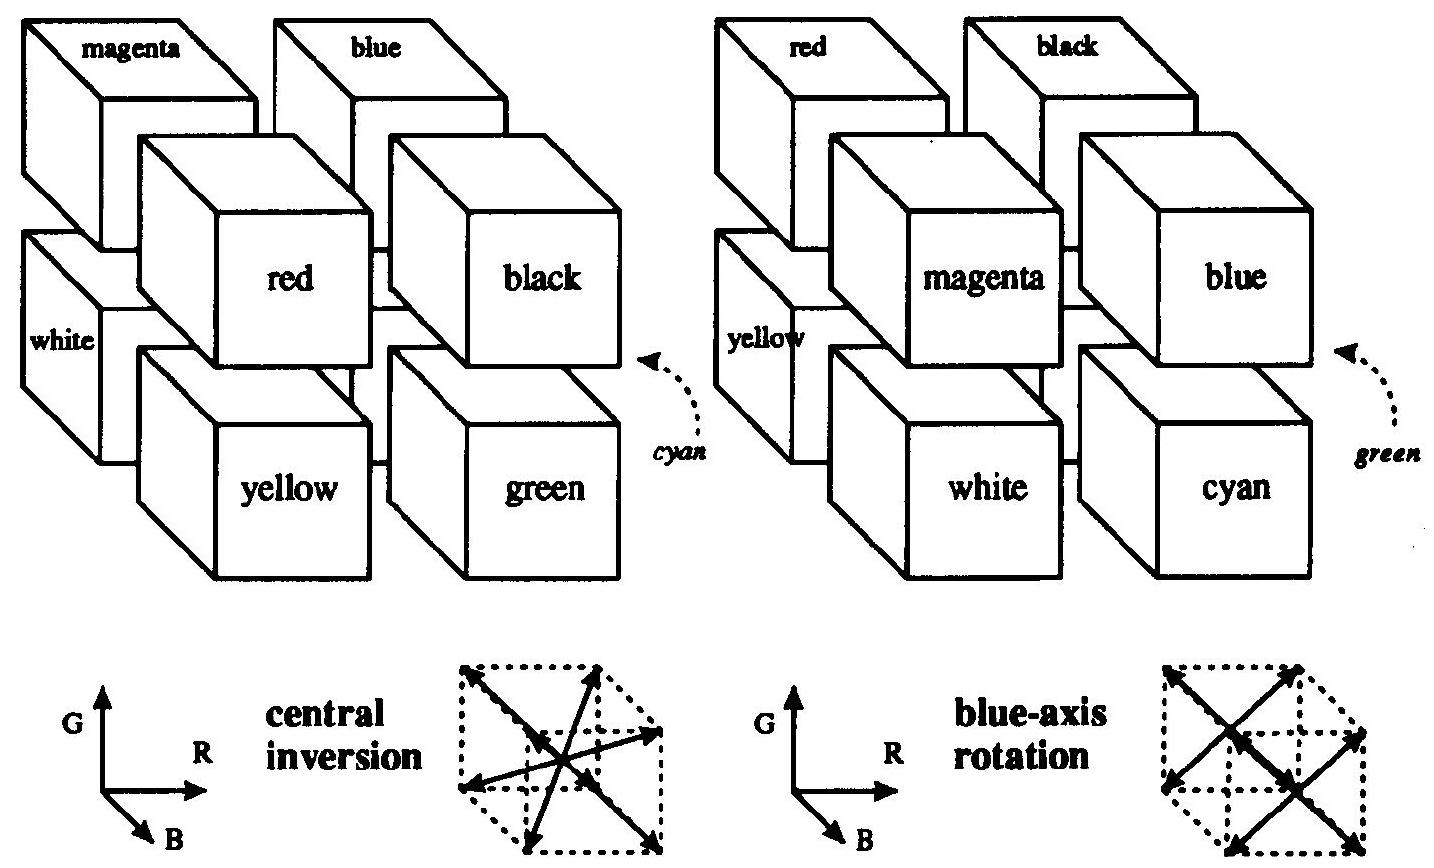
\includegraphics[max width=\textwidth]{2022_11_30_0cbb01a33d99487fc27fg-111}
\end{center}

Figure 1

covered implicitly. The alternate generic macro is

$$
\text { macro pixelflip2(x) } \quad \mathrm{x}:=\mathrm{x} \text { bit-xor } 34181 \text { hex } 8585
$$

For 24-bit color, preservation of blue means that subcubes no longer swap through central inversion (Fig. la), but are instead rotated a half-turn about the blue axis in "Ferris-wheel" fashion (lb). This creates a pair of opponent colors (red, green) for which the human visual system is highly responsive, plus pairs (blue, white), (cyan, magenta) and (yellow, black). The alternate macro supports the use of short, 16-bit integers in the reversal.

See also G1, 215; G1, 219; G1, 233; G1, 249.

\section{NONUNIFORM RANDOM POINT SETS VIA WARPING}
\begin{center}

\includegraphics[max width=\textwidth]{2022_11_30_0cbb01a33d99487fc27fg-112}
\end{center}

We often want to generate sets of random or pseudorandom points on the unit square for applications such as distribution ray tracing. There are several methods for doing this, such as jittering and Poisson disk sampling. These methods give us a set of $\mathrm{N}$ reasonably equidistributed points on the unit square: $\left(u_{1}, v_{1}\right)$ through $\left(u_{N^{\prime}}, v_{N}\right)$.

Sometimes, our sampling space may not be square (e.g., a circular lens) or may not be uniform (e.g., a filter function centered on a pixel). It would be nice if we could write a mathematical transformation that would take our equidistributed points $\left(\mathrm{u}_{\mathrm{i}}, \mathrm{v}_{\mathrm{i}}\right)$ as input, and output a set of points in our desired sampling space with our desired density. For example, to sample a camera lens, the transformation would take $\left(\mathrm{u}_{\mathrm{i}}, \mathrm{v}_{\mathrm{i}}\right)$ and output $\left(r_{i}, \theta_{i}\right)$ such that the new points were approximately equidistributed on the disk of the lens.

It turns out that such transformation functions are well known in the field of Monte Carlo integration. A table of several transformations useful for computer graphics is given in Table I. The method for generating such transformations is discussed for the rest of this article. Note that several of these transformations can be simplified for simple densities. For example, to generate directions with a cosine distribution, use the Phong density with $\mathrm{n}=1$. To generate points on the unit hemisphere, use the sector on the unit sphere density with $\theta_{1},=0, \theta_{2}=\pi / 2, \varphi_{1}=0$, and $\varphi_{2}=\pi$.

For Monte Carlo methods we must often generate random points according to some probability density function, or random rays according to a directional probability density. In this section a method for one and two dimensional random variables is described. The discussion closely follows that of Shreider (1966).

\section{II.7 NONUNIFORM RANDOM POINTS VIA WARPING}
Table 1. Some Useful Transformation. ${ }^{a}$.

\begin{center}
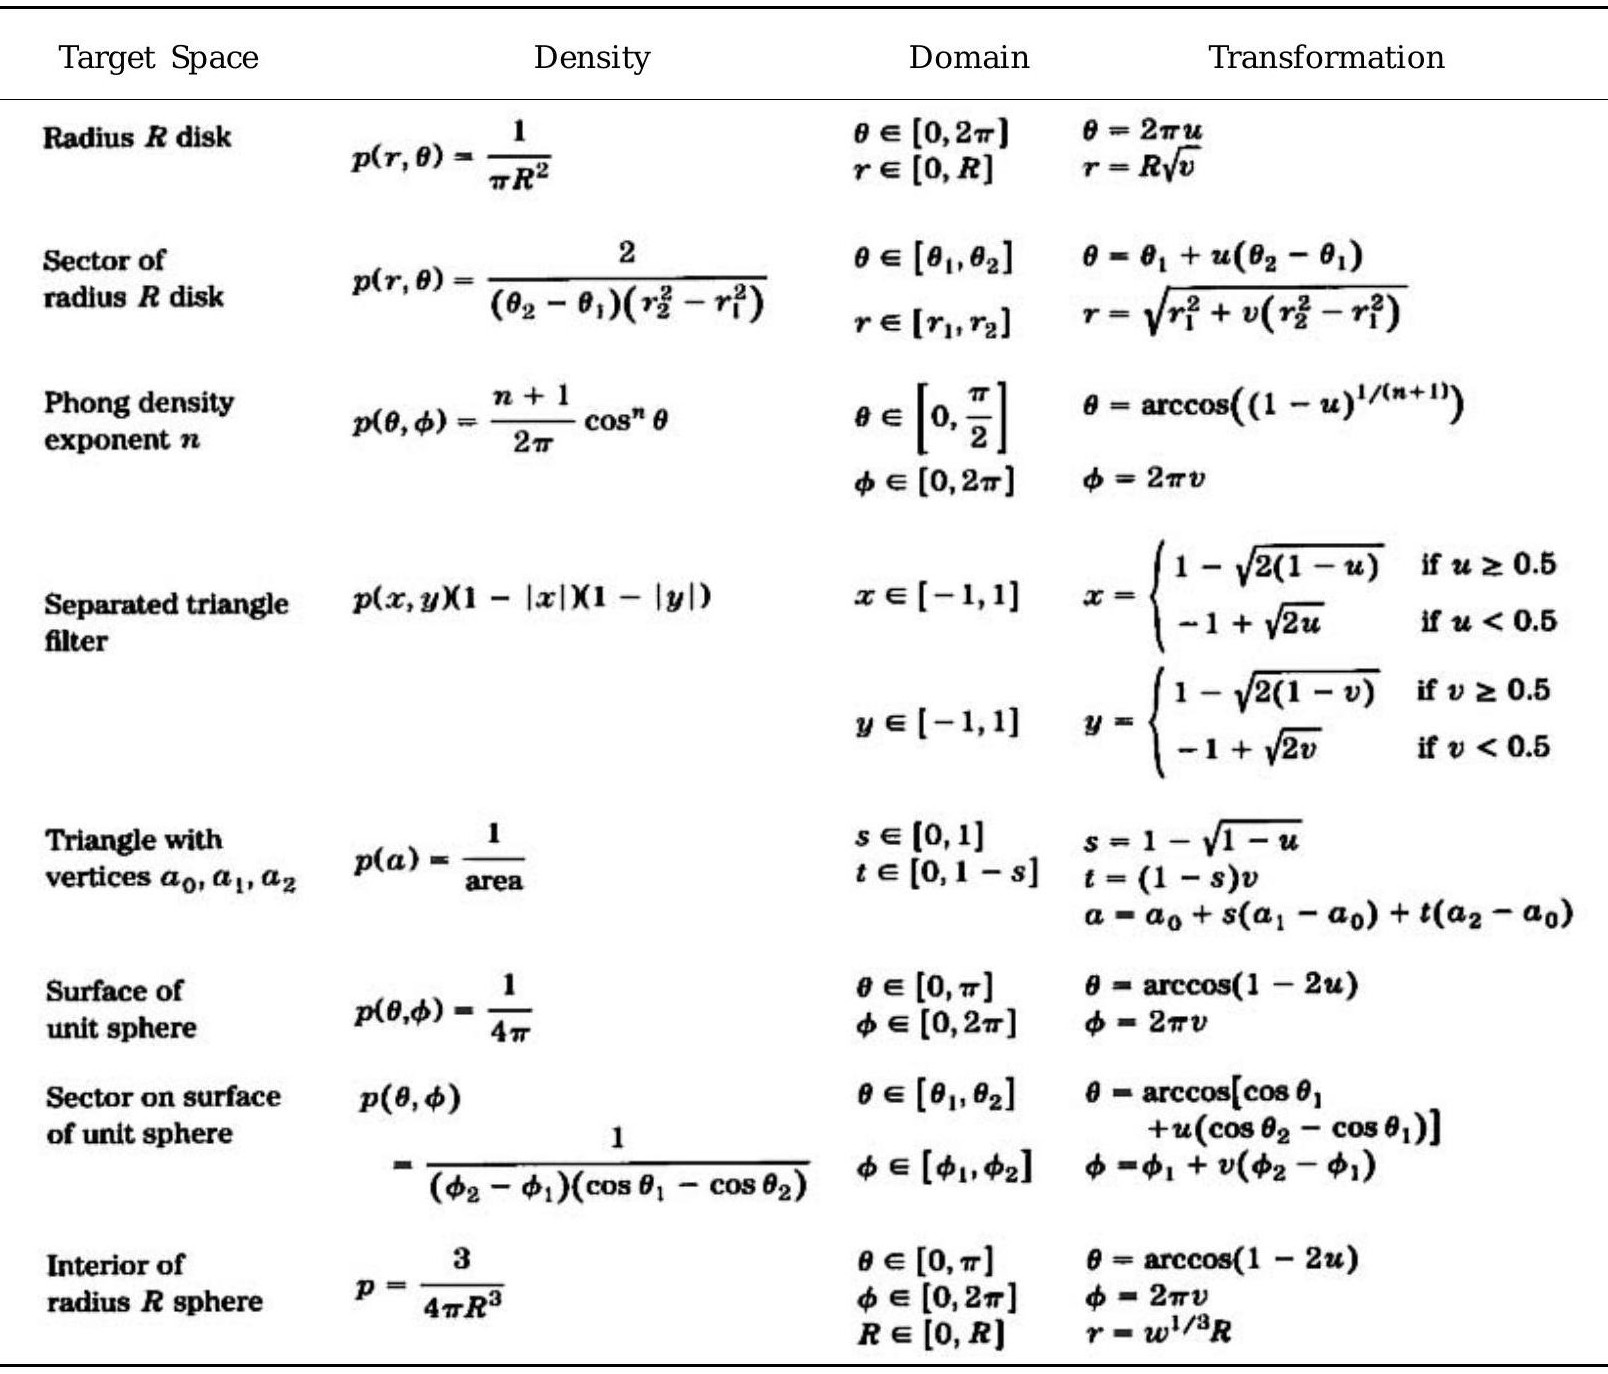
\includegraphics[max width=\textwidth]{2022_11_30_0cbb01a33d99487fc27fg-113}
\end{center}

a The symbols $u, v$, and $w$ represent instances of uniformly distributed random variables ranging over [0, 1].

If the density is a one-dimensional $\mathrm{f}(\mathrm{x})$ defined over the interval $\mathrm{x} \in[\mathrm{a}, \mathrm{b}]$, then we can generate random numbers $\alpha_{\mathrm{i}}$ that have density $\mathrm{f}$ from a set of uniform random numbers $\xi_{\mathrm{i}}$, where $\xi_{\mathrm{i}} \in[0,1]$. To do this we need the probability distribution function $\mathrm{F}(\mathrm{x})$ :

$$
F(x)=\int_{a} f\left(x^{\prime}\right) d \mu\left(x^{\prime}\right)
$$

\section{II.7 NONUNIFORM RANDOM POINTS VIA WARPING}
To get $\alpha_{\mathrm{i}}$ we simply transform $\xi_{\mathrm{i}}$ :

$$
\alpha_{\mathrm{i}}=\mathrm{F}^{-1}\left(\mathrm{x}_{\mathrm{i}}\right) \text {, }
$$

where $\mathrm{F}^{-1}$ is the inverse of $\mathrm{F}$. If $\mathrm{F}$ is not analytically invertible, then numerical methods will suffice because an inverse exists for all valid probability distribution functions.

If we have a two-dimensional density $(\mathrm{x}, \mathrm{y})$ defined on [a, b: c, d], then we need the two-dimensional distribution function:

$$
F(x, y)=\int_{c}^{y} \int_{a}^{\prime} f\left(x^{\prime}, y^{\prime}\right) d \mu\left(x^{\prime}, y^{\prime}\right) .
$$

We first choose an $\mathrm{x}_{\mathrm{i}}$ using the marginal distribution $\mathrm{F}(\mathrm{x}, \mathrm{d})$, and then choose $y_{i}$ according to $F\left(x_{i}, y\right) / F\left(x_{i}, d\right)$. If $F(x, y)$ is separable (expressable as $g(\mathrm{x}) \mathrm{h}(\mathrm{y}))$, then the one-dimensional techniques can be used on each dimension.

As an example, to choose reflected ray directions for zonal calculations or distributed ray tracing, we can think of the problem as choosing points on the unit sphere or hemisphere (since each ray direction can be expressed as a point on the sphere). For example, suppose that we want to choose rays according to the density

$$
\mathrm{p}(\theta, \varphi)=\frac{\mathrm{n}+1}{2 \pi} \cos ^{\mathrm{n}} \theta,
$$

where $\mathrm{n}$ is a Phong-like exponent; $\theta$ is the angle from the surface normal and $\theta \in[0, \pi / 2]$ (is on the upper hemisphere); and $\varphi$ is the azimuthal angle $(\varphi \in[0,2 \pi])$. The distribution function is

$$
\mathrm{P}(\theta, \varphi)=\int_{0}^{\varphi} \int_{0}^{\theta} \mathrm{p}\left(\theta, \varphi^{\prime}\right) \sin \theta \mathrm{d} \theta \mathrm{d} \varphi^{\prime} .
$$

The $\sin \theta$ term arises because $\mathrm{d} \omega=\sin \theta \mathrm{d} \theta \mathrm{d} \varphi$ on the sphere. When the marginal densities are found, $p$ (as expected) is separable, and we find that a $\left(r_{1}, r_{2}\right)$ pair of uniform random numbers can be transformed to a direction by

$$
(\theta, \varphi)=\left(\arccos \left(\left(1-r_{1}\right)^{1 /(n+1)}\right), 2 \pi r_{2}\right) .
$$

\section{II.7 NONUNIFORM RANDOM POINTS VIA WARPING}
Typically, we want a directional $(\theta, \varphi)$ pair to be with respect tosomeunit vector $\mathrm{y}$ (as opposed to the $\mathrm{z}$ axis). To do this we can first convert the angles to a unit vector a:

$$
\mathrm{a}=(\cos \varphi \sin \theta, \sin \varphi \sin \theta, \cos \theta) .
$$

We can then transform a to be an a' with respect to $\psi$ by multiplying a by a rotation matrix $\mathrm{R}\left(\mathrm{a}^{\prime}=\mathrm{Ra}\right.$ ). This rotation matrix is simple to write down:

$$
R=\begin{array}{lll}
u_{x} & v_{x} & w_{x} \\
u_{y} & v_{y} & w_{y} \\
u_{z} & v_{z} & w_{z}
\end{array}
$$

where $u=\left(u_{x^{\prime}} u_{y^{\prime}} u_{z}\right), v=\left(v_{x^{\prime}} v_{y^{\prime}} v_{z}\right), w=\left(w_{x^{\prime}} w_{y^{\prime}}, w_{z}\right)$, form a basis (an orthonormal set of unit vectors where $u=\mathrm{v} \times \mathrm{w}, \mathrm{v}=\mathrm{w} \times \mathrm{u}$, and $\mathrm{w}=\mathrm{u} \times \mathrm{v}$ ) with the constraint that $\mathrm{w}$ is aligned with $\psi$ :

$$
\mathrm{w}=\frac{\psi}{|\psi|} .
$$

To get $u$ and $v$, we need to find a vector $t$ that is not colinear with $w$. To do this simply set $t$ equal to $\mathrm{w}$ and change the smallest magnitude component of $\mathrm{t}$ to one. The $\mathrm{u}$ and $\mathrm{v}$ follow easily:

$$
\begin{aligned}
&\mathrm{u}=\frac{\mathrm{t} \times \mathrm{w}}{|\mathrm{t} \times \mathrm{w}|}, \\
&\mathrm{v}=\mathrm{w} \times \mathrm{u} .
\end{aligned}
$$

This family of techniques is very useful for many sampling applications. Unfortunately, some sampling spaces (e.g., the surface of a dodecahedron) are not naturally dealt with using the methods in this gem. Special purpose or, as a last resort, rejection techniques are then called for.

See also G1, 438.

\begin{center}
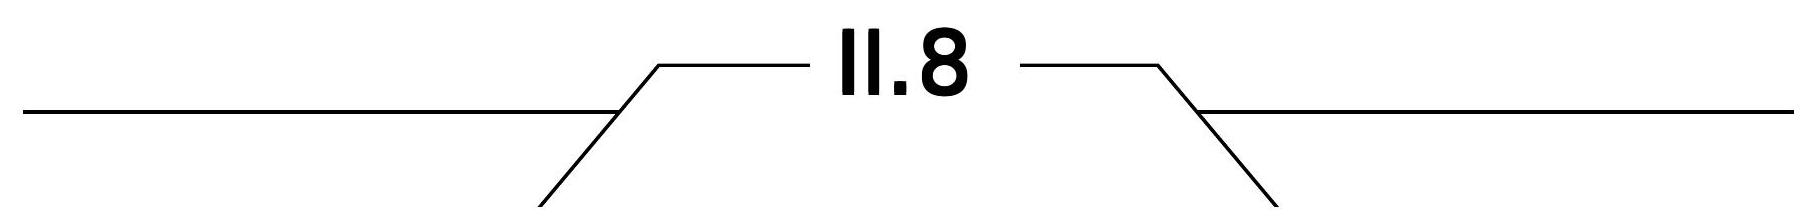
\includegraphics[max width=\textwidth]{2022_11_30_0cbb01a33d99487fc27fg-116}
\end{center}

\section{CROSS PRODUCT IN FOUR DIMENSIONS AND BEYOND}
\begin{center}
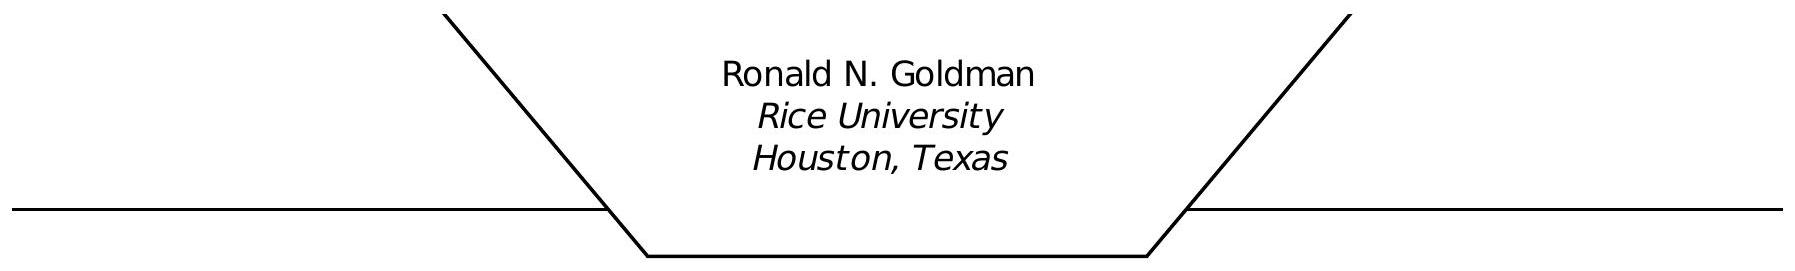
\includegraphics[max width=\textwidth]{2022_11_30_0cbb01a33d99487fc27fg-116(1)}
\end{center}

\section{Introduction}
Cross product is one of the gods' great gifts to mankind. It has many applications in mathematics, physics, engineering, and, of course, computer graphics. Normal vectors, rotations, curl, angular momentum, torque, and magnetic fields all make use of the cross product.

Given two linearly independent vectors $\mathrm{u}$ and $\mathrm{v}$ in three dimensions, their cross product is the vector $u \times v$ perpendicular to the plane of $u$ and $\mathrm{v}$, oriented according to the right-hand rule, with length equal to $|\mathrm{u}||\mathrm{v}| \sin \theta$, where $\Theta$ is the angle between $u$ and $v$. In rectangular coordinates, the cross product can be computed from the simple determinant formula

$$
u \times v=\left|\begin{array}{ccc}
\mathbf{i} & \mathbf{j} & \mathbf{k} \\
\mathrm{u}_{1} & \mathrm{u}_{2} & \mathrm{u}_{3} \\
\mathrm{v}_{1} & \mathrm{v}_{2} & \mathrm{v}_{3}
\end{array}\right| .
$$

Equivalently,

$$
u \times v=\left(u_{2} v_{3}-u_{3} v_{2}, u_{3} v_{1}-u_{1} v_{3^{\prime}} u_{1} v_{2^{\prime}}-u_{2} v_{1}\right) \text {. }
$$

At first glance, cross product seems to be an artifact of three dimensions. In three dimensions the normal direction to the plane determined by two vectors is unique up to sign, but in four dimensions there are a whole plane of vectors normal to any given plane. Thus, it is unclear how to define the cross product of two vectors in four dimensions. What then

\section{II.8 CROSS PRODUCT IN FOUR DIMENSIONS AND BEYOND}
is the analogue of the cross product in four dimensions and beyond? The goal of this gem is to answer this question.

\section{Tensor Product}
There is a way to look at the cross product that is more instructive than the standard definition and that generalizes readily to four dimensions and beyond. To understand this approach, we need to begin with the notion of the tensor product of two vectors $u$, v.

The tensor product $u \otimes v$ is defined to be the square matrix

$$
\mathrm{u} \otimes \mathrm{v}=\mathrm{u}^{\mathrm{t}} * \mathrm{v},
$$

where the superscript $\mathrm{t}$ denotes transpose and $*$ denotes matrix multiplication. Equivalently,

$$
(u \otimes v)_{i j}=\left(u_{i}, v_{j}\right) .
$$

Notice that for any vector $\mathrm{w}$,

$$
\mathrm{w}(\mathrm{u} \otimes \mathrm{v})=(\mathrm{w} \cdot \mathrm{u}) \mathrm{v} .
$$

Thus, the tensor product is closely related to the dot product.

Like dot product, the tensor product makes sense for two vectors of arbitrary dimension. Indeed, the tensor product shares many of the algebraic properties of the dot product. However, unlike the dot product, the tensor product is not communative. That is, in general,

$$
u \otimes v \neq v \otimes u \quad \text { because } u_{i} v_{j} \neq u_{j} v_{i}
$$

Applications of the tensor product of two vectors to computer graphics are given in Goldman (1990, 1991).

\section{Wedge Product}
The wedge product of two vectors $u$ and $v$ measures the noncommutativity of their tensor product. Thus, the wedge product $u \wedge v$ is the square

\section{II.8 CROSS PRODUCT IN FOUR DIMENSIONS AND BEYOND}
matrix defined by

$$
u \wedge v=u \otimes v-v \otimes u .
$$

Equivalently,

$$
(u \wedge v)_{i j}=\left(u_{i} v_{j}-u_{j} v_{i}\right) .
$$

Like the tensor product, the wedge product is defined for two vectors of arbitrary dimension. Notice, too, that the wedge product shares many properties with the cross product. For example, it is easy to verify directly from the definition of the wedge product as the difference of two tensor products that:

$\mathrm{u} \wedge \mathrm{u}=0$,

$\mathrm{u} \wedge \mathrm{v}=-\mathrm{v} \wedge \mathrm{u}$

(anticommutative),

$\mathrm{u} *(\mathrm{v} \wedge \mathrm{w}) \neq(\mathrm{u} \wedge \mathrm{v}) * \mathrm{w}^{\mathrm{t}}$

(nonassociative),

$\mathrm{u} \wedge \mathrm{cv}=\mathrm{c}(\mathrm{u} \wedge \mathrm{v})=(\mathrm{cu}) \wedge \mathrm{v}$,

$\mathrm{u} \wedge(\mathrm{v}+\mathrm{w})=\mathrm{u} \wedge \mathrm{v}+\mathrm{u} \wedge \mathrm{w}$

(distributive),

$\mathrm{u} *(\mathrm{v} \wedge \mathrm{w})+\mathrm{v} *(\mathrm{w} \wedge \mathrm{u})+\mathrm{w} *(\mathrm{u} \wedge \mathrm{v})=0$

(Jacobi identity),

$\mathrm{r} *(\mathrm{u} \wedge \mathrm{v}) * \mathrm{~s}^{\mathrm{t}}=(\mathrm{r} \cdot \mathrm{u})(\mathrm{s} \cdot \mathrm{v})-(\mathrm{r} \cdot \mathrm{v})(\mathrm{s} \cdot \mathrm{u})$

(Lagrange identity).

The wedge product also shares some other important properties with the cross product. The defining characteristics of the cross product are captured by the formulas

$$
\begin{gathered}
u \cdot(u \times v)=v \cdot(u \times v)=0, \\
|u \times v|=|u|^{2}|v|^{2} \sin ^{2} \Theta .
\end{gathered}
$$

By the Lagrange identity, the wedge product satisfies the analogous

\section{II.8 CROSS PRODUCT IN FOUR DIMENSIONS AND BEYOND}
identities:

$$
\begin{aligned}
&\mathrm{u} *(\mathrm{u} \wedge \mathrm{v}) * \mathrm{u}^{\mathrm{t}}=\mathrm{v} *(\mathrm{u} \wedge \mathrm{v}) * \mathrm{v}^{\mathrm{t}}=0, \\
&\mathrm{u} *(\mathrm{u} \wedge \mathrm{v}) * \mathrm{v}^{\mathrm{t}}=(\mathrm{u} \cdot \mathrm{u})(\mathrm{v} \cdot \mathrm{v})-(\mathrm{u} \cdot \mathrm{v})^{2}=\left.\left.|\mathrm{u}|\right|^{2} \mathrm{v}\right|^{2} \sin ^{2} \Theta
\end{aligned}
$$

A variant of the last identity can be generated by defining the norm of a matrix $M$ to be

$$
|M|^{2}={ }_{2}^{1} \sum_{i j}\left(M_{i j}\right)^{2} .
$$

Then by direct computation it is easy to verify that

$$
|u \wedge v|^{2}=(u \cdot u)(v \cdot v)-(u \cdot v)^{2}=|u|^{2}|v|^{2} \sin ^{2} \Theta .
$$

In addition, the cross product identity

$$
(\mathrm{u} \times \mathrm{v}) \times \mathrm{w}=(\mathrm{w} \cdot \mathrm{u}) \mathrm{v}-(\mathrm{w} \cdot \mathrm{v}) \mathrm{u}
$$

has the wedge product analogue

$$
\mathrm{w} \cdot(\mathrm{u} \wedge \mathrm{v})=(\mathrm{w} \cdot \mathrm{u}) \mathrm{v}-(\mathrm{w} \cdot \mathrm{v}) \mathrm{u} .
$$

The cross product can be used to test for vectors perpendicular to the plane of $u$ and $v$ because

$$
\mathrm{w} \times(\mathrm{u} \times \mathrm{v})=0 \Leftrightarrow \mathrm{w} \perp \mathrm{u}, \mathrm{v} .
$$

Similarly, the wedge product recognizes vectors perpendicular to the plane determined by $u$ and $v$ because by (1),

$$
\mathrm{w} *(\mathrm{u} \wedge \mathrm{v})=0 \Leftrightarrow(\mathrm{w} \cdot \mathrm{u})=(\mathrm{w} \cdot \mathrm{v})=0 \Leftrightarrow \mathrm{w} \perp \mathrm{u}, \mathrm{v} .
$$

Moreover, in three dimensions,

$$
u \Lambda v=\left|\begin{array}{ccc}
0 & u_{1} v_{2}-u_{2} v_{1} & u_{1} v_{3}-u_{3} v_{1} \\
u_{2} v_{1}-u_{1} v_{2} & 0 & u_{2} v_{3}-u_{3} v_{2} \\
u_{3} v_{1}-u_{1} v_{3} & u_{3} v_{2}-u_{2} v_{3} & 0
\end{array}\right|
$$

\section{II.8 CROSS PRODUCT IN FOUR DIMENSIONS AND BEYOND}
Thus, in three dimensions the entries of the wedge product matrix $u \wedge v$ are, up to sign, the same as the components of the cross product vector $\mathrm{u} \times \mathrm{v}$. This observation explains why wedge product and cross product share so many algebraic properties.

In three dimensions we are really very lucky. The matrix $u \wedge v$ is antisymmetric so, up to sign, it has only three unique entries. This property allows us to identify the matrix $u \wedge v$ with the vector $u \times v$. Nevertheless, there is something very peculiar about the vector $u \times v$. If $\mathrm{u}$ and $\mathrm{v}$ are orthogonal unit vectors, then the vectors $u, v, u \times v$ form a right-handed coordinate system. But if $\mathrm{M}$ is the linear transformation that mirrors vectors in the $u, v$ plane, then $\{u \cdot M, v \cdot M,(u \times v) \cdot M\}=$ $\{u, v,-u \times v\}$ forms a left-handed coordinate system. Thus, (u $\cdot M) \times$ $(\mathrm{v} \cdot \mathrm{M}) \neq(\mathrm{u} \times \mathrm{v}) \cdot \mathrm{M}$, so $\mathrm{u} \times \mathrm{v}$ does not really transform as a vector. This anomaly should alert us to the fact that cross product is not really a true vector. In fact, cross product transforms more like a tensor than a vector.

In higher dimensions we are not nearly so lucky. For example, in four dimensions the antisymmetric matrix $u \wedge v$ has, up to sign, six, not four, distinct entries. Thus, the matrix $u \wedge v$ cannot be identified with a four-dimensional vector. In $\mathrm{n}$ dimensions, the antisymmetric matrix $\mathrm{u} \wedge \mathrm{v}$ has $n(n-1) / 2$ unique entries. But $n(n-1) / 2 \neq n$ unless $n=0,3$. Thus, only in three dimensions can we identify the wedge product of two vectors with a vector of the same dimension. In general, the wedge product is an antisymmetric 2-tensor. This antisymmetric tensor shares many of the important algebraic properties of the cross product, and thus it is a natural generalization of the cross product to four dimensions and beyond.

\section{Acknowledgment}
I would like to thank Joe Warren for pointing out that the formula for the length of the cross product $u \times v$ has a direct analogue in the formula for the norm of the wedge product $u \wedge v$.


\begin{center}
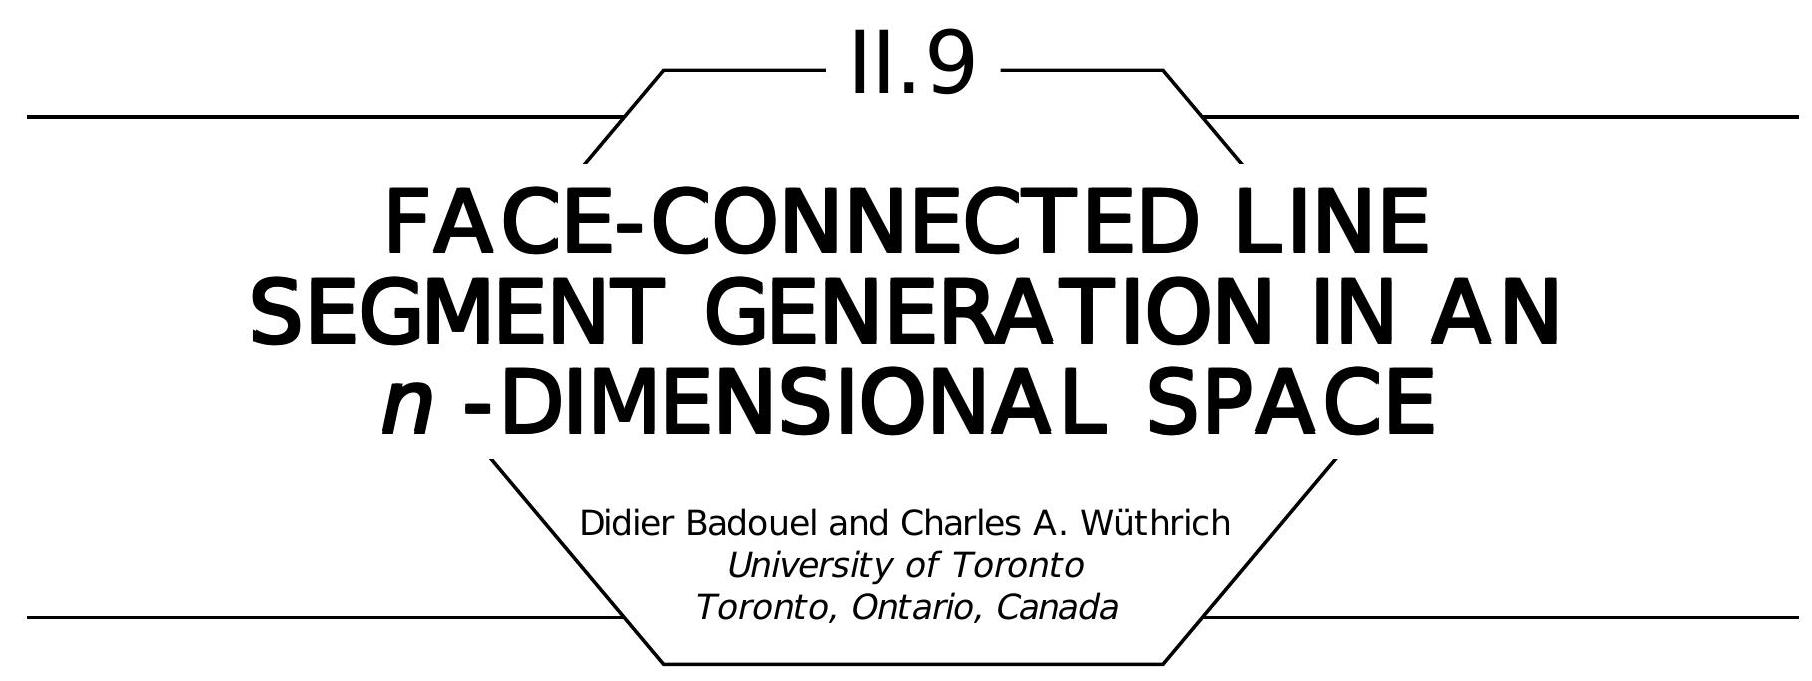
\includegraphics[max width=\textwidth]{2022_11_30_0cbb01a33d99487fc27fg-121}
\end{center}

In the early days of Computer Graphics, straight line rasterization was developed to render segments onto the raster plane. Later, three-dimensional segment discretization had to be developed to keep track of the path of a ray in the object space. These algorithms generate a connected sequence that represents the segment in the discrete space; moreover, they define a path in which the directions are uniformly distributed. An extension to higher-dimensional spaces is suited for applications ranging from line generation in a time-space coordinate system to the incremental generation of a discrete simultaneous linear interpolation of any number of variables.

This gem presents an algorithm that generates a face-connected line segment in discrete n-dimensional spaces. In two dimensions, the algorithm introduced below coincides with any classical 4-connected straight line drawing algorithm. Among all discrete segments joining two points, this algorithm produces one in which the directions are uniformly distributed. A definition of uniform distribution is given below.

Consider an n-dimensional lattice, or hyperlattice, i.e., the set of all points $\mathrm{P}=\left(\mathrm{p}_{0}, \mathrm{p}_{1}, \ldots, \mathrm{p}_{\mathrm{n}-1}\right)$ of $\mathbf{Z}^{\mathrm{n}}$ : Neighbourhood relations can be defined between the Voronoi hypervroxel associated with each point of the hyperlattice. In fact, only voxels having a hyperface in common, i.e., corresponding to hyperlattice points having $\mathrm{n}-1$ coordinates in common, will be considered here as neighbours. In a two-dimensional lattice, such neighbourhood relation is the well-known 4 -connection, while in the three-dimensional space it leads to 6-connection. The neighbourhood relations among the hyperlattice points introduce a rasterization proce- dure for curves into the hyperlattice: A rasterization of a curve is in fact a path of neighbouring lattice points.

Consider two hyperlattice points $P=\left(p_{0^{\prime}}, p_{1}, \ldots, p_{n-1}\right)$ and $Q=$ $\left(q_{0^{\prime}} q_{1}, \ldots, q_{n-1}\right)$. Let $n_{i}=\left|q_{i}-p_{i}\right|$ Then a face-connected shortest path between $\mathrm{P}$ and $\mathrm{Q}$ requires $\mathrm{m}=\sum \mathrm{n}_{\mathrm{i}}$ steps. The hyperline points are the points of coordinates $x_{i}=\left(q_{i}-p_{i}\right) t+p_{i}$, with $t \in[0,1]$. The parameter $t$ introduces an ordering on the points of the straight line. Consider the straight line points $P_{i, h_{1}}$ obtained for $t=h_{i} / n_{i}$, where $h_{j}=1, \ldots, n_{i}$, and order them in increasing order of their corresponding parameter value. Whenever an ambiguity occurs, and two parameter values $h_{\mathrm{j}} / \mathrm{n}_{\mathrm{i}}$ and $h_{\mathrm{j}} / \mathrm{n}_{\mathrm{j}}$ coincide, an arbitrary order has to be chosen. In other words, the segment $\mathrm{PQ}$ is subdivided into $\mathrm{n}_{\mathrm{i}}$ parts for each dimension i, and the points obtained on the straight line segment are ordered by increasing values of the parameter t. When two subdivision points coincide, the one corresponding to the smaller dimension is considered to precede the other one.

The resulting set is a finite ordered set of the segment points $P_{i, h_{i}}$, which can be renamed as $A_{0^{\prime}} A_{1}, \ldots, A_{m-1}$ Consider the finite path built by taking the sequence of directions $\left\{a_{k}\right)_{k=0, \ldots, m-1}$, such that each direction $a_{k}$ corresponds to the point $A_{k}=P_{a_{k}, 1}$, for some l. Such a path is said to be uniformly distributed with respect to the directions that constitute it. It is clear that in such a path the occurrences of the different directions that have to appear in it are as evenly spaced as possible in the chain. Moreover, if we follow the previously defined path from the point $\mathrm{P}$, the point $\mathrm{Q}$ shall be reached.

Whenever the hyperface-connected rasterization onto the n-dimensional hyperlattice of a straight line segment joining two hyperlattice points is computed, the result is a hyperface-connected path joining the two points. This path is uniformly distributed among all directions. A simplified version of the routing algorithm can be therefore summarized as follows. For each direction $i$, an integer counter $d_{i}$ is used. In order to generate the straight line between the two points $P$ and $Q$, the values of $\mathrm{n}_{\mathrm{i}}$ are computed. Their least common multiple $\mathrm{l}=\mathrm{LCM}\left(\mathrm{n}_{\mathrm{i}}\right)$ is evaluated, ${ }^{1}$ and the values of $\mathrm{n}_{\mathrm{i}}^{\prime \prime}=1 / \mathrm{n}_{\mathrm{i}}$ are computed. To obtain only integer

${ }^{1}$ In fact, either a low-complexity method in $\mathrm{O}(\mathrm{n} \log \mathrm{k})$ based on a table lookup or a simple common multiple can be used here. computations, the values of $n_{i}^{\prime}=2 n^{\prime \prime}$ are used. The cells $d_{i}$ are initialized to the value $n_{i}^{\prime} / 2$. This initialization has to be made, otherwise the path generated corresponds to another rasterization scheme. At each step, $\mathrm{n}_{\mathrm{i}}^{\prime}$ is added to the di with the smallest value, and the ith signed direction is generated. The generation procedure is repeated until all $d_{i}$ have reached the value $2 l+n_{i}^{\prime \prime}$. which is equivalent to $\forall i, d_{i} \geq 2 l$.\\




\end{CJK}
\chapter{模型和变换矩阵}
本章中的大多数宝石都与变换有关:如何组合、分解和操作它们。第一个Gem描述了如何使用四元数表示在两个方向之间进行插值,并在插值的末尾添加了额外的自旋。第五个Gem是第一个的有用伴侣,因为它讨论了与插值发生时的转换选择有关的问题。第七篇Gem描述了一种替代的插值技术,使用B\'ezier曲线。

第二个和第三个gem讨论了如何将复杂的转换分解为更简单的组件。本节中的第四个和第六个Gems描述了产生旋转的两种互补技术,它们在某种意义上是随机的,并且在方向上均匀分布。这些宝石是对以前的宝石的改进。

本节中的最后一个Gem是征求意见稿,为那些对基于物理的建模感兴趣的人提供了有用的信息。本文给出了超二次椭球和环面体积和质量性质的封闭形式表达式,并讨论了惯性张量的计算和使用。

\newpage
\section{带有额外自旋的四元数插值}
\begin{center}
\small{
Jack Morrison\\
Digital Insight\\
Evergreen, Colorado}
\end{center}

Quaternions are handy for representing the orientation or rotation of a 3-D object (Shoemake, 1985). The "Slerp" operation (spherical linear interpolation) interpolates between two quaternions at a constant speed, using the most direct rotational path between the orientations. An animator may, however, want the interpolation to provide extra spins along the same path (complete revolutions about the same axis-see Fig. 1). This Gem gives a simple formula for doing this, derived with the help of Steven Gabriel.

Given two unit quaternions $\mathbf{A}$ and $\mathbf{B}$, and an interpolation parameter $\alpha$ ranging from 0 to 1 , the basic Slerp equation is

$$
\operatorname{Slerp}(\mathbf{A}, \mathbf{B} ; \alpha)=\mathbf{A}\left(\mathbf{A}^{-1} \mathbf{B}\right)^{\alpha} .
$$

An easier-to-implement equation uses the angle $\theta$ between the quaternions:

$$
\begin{aligned}
\theta &=\operatorname{acos}(\mathbf{A} \cdot \mathbf{B}) \\
\operatorname{Slerp}(\mathbf{A}, \mathbf{B} ; \alpha) &=\frac{\sin (\theta-\alpha \theta)}{\sin \theta} \mathbf{A}+\frac{\sin (\alpha \theta)}{\sin \theta} \mathbf{B} .
\end{aligned}
$$

To include $\mathrm{k}$ additional spins, determine

$$
\varphi=\theta+\mathrm{k} \pi,
$$


\begin{center}
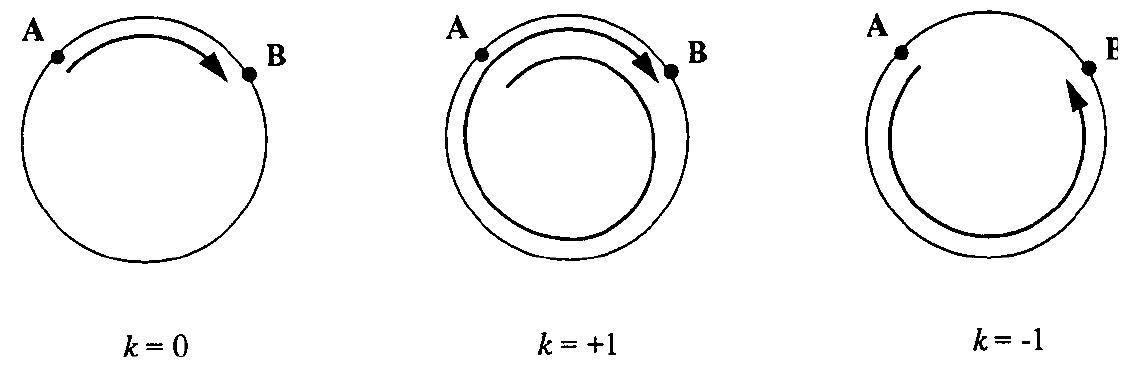
\includegraphics[max width=\textwidth]{2022_11_30_0cbb01a33d99487fc27fg-129}
\end{center}

Figure 1. Slerp (A, B) with $\mathrm{k}$ additional spins.

then

$$
\operatorname{Slerp}(\mathbf{A}, \mathbf{B}, \mathrm{k} ; \boldsymbol{\alpha})=\frac{\sin (\theta-\alpha \varphi)}{\sin \theta} \mathbf{A}+\frac{\sin (\alpha \varphi)}{\sin \theta} \mathbf{B}
$$

Figure 1 shows the effect of $\mathrm{k}$, viewing orientations $\mathbf{A}$ and $\mathbf{B}$ along the rotation axis. For $\mathrm{k}=0$, $\mathrm{f}$ equals $\mathrm{q}$, the equation reduces to the original form, and the interpolation follows the shortest circular path from A to $\mathbf{B}$. For $\mathrm{k}=+1$, one full additional rotation is generated as a goes from 0 to 1. For $\mathrm{k}=-1$, the interpolation goes the "long" way around.

The C implementation first checks if $\mathbf{A}$ and $\mathbf{B}$ are on opposite hemispheres $(\cos \theta<0$ ). If so, the interpolation is modified to use the negation of B (which represents the same orientation as B itself), to ensure that the shortest rotation path is taken. It also checks whether A and $\mathbf{B}$ are the same, so that $\sin \theta=0$, and no axis is defined for spinning. If $\mathbf{A}$ and $\mathbf{B}$ represent orientations 180 degrees apart, all rotation paths are the same length, but the quaternions still define an axis for spinning. Note that for a given $\mathbf{A}, \mathbf{B}$, and $\mathrm{k}$, the quantities $\theta, \varphi$, and $\sin \theta$ could be computed once outside the interpolation loop for efficiency.

See also G1, 498.\\
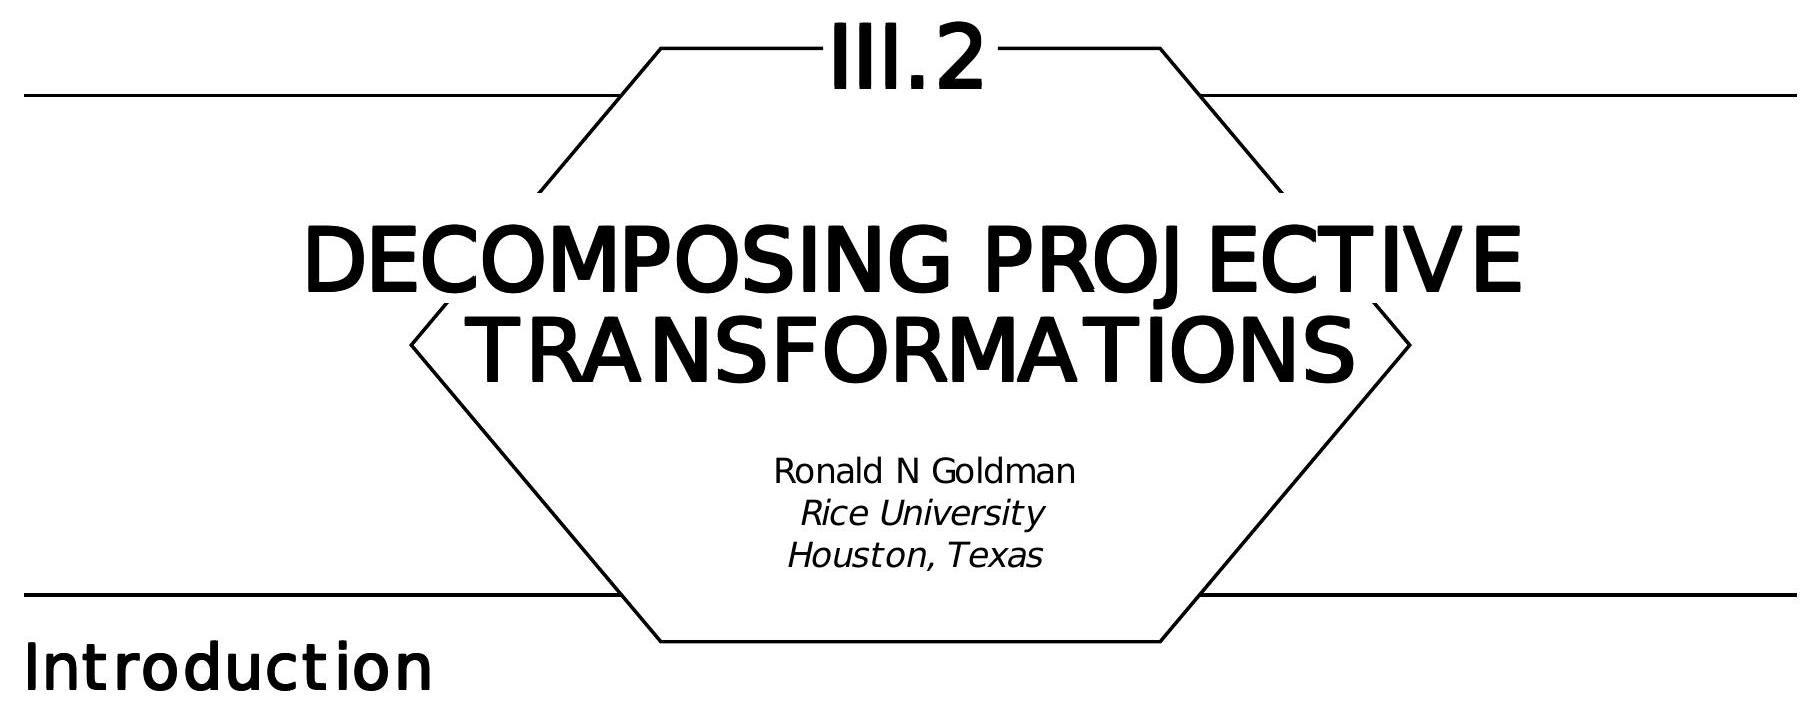
\includegraphics[max width=\textwidth, center]{2022_11_30_0cbb01a33d99487fc27fg-130}

In another Gem (III.3) we show how to decompose linear and affine transformations of three-dimensional space into the products of scale, shears, rotations, translations, and projections. The goal of this gem is to demonstrate how to decompose an arbitrary projective transformation of three-dimensional space into simple, geometrically meaningful factors. For an alternative approach, see Thomas (1991).

Let us begin by recalling the difference between linear, affine, and projective transformations. Consider a point $\mathrm{P}$ with coordinates $(\mathrm{x}, \mathrm{y}, \mathrm{z})$, and let $\mathrm{P}_{\text {new }}$ with coordinates $\left(\mathrm{x}_{\text {new }}, \mathrm{y}_{\text {new }}, \mathrm{z}_{\text {new }}\right.$ ) denote the new transformed point. Formulas that express the new coordinates $\mathrm{x}_{\text {new }}, \mathrm{y}_{\text {new }}, \mathrm{z}_{\text {new }}$ in terms of the original coordinates $\mathrm{x}, \mathrm{y}, \mathrm{z}$ are given by the following equations:

Linear:

Affine:

Projective:

$$
\begin{aligned}
&\mathrm{x}_{\text {new }}=a x+b y+c z, \\
&x_{\text {new }}=a x+b y+c z+d, \\
&x_{\text {new }}=(a x+b y+c z+d) /(\alpha x+\beta y+\gamma z+\delta),
\end{aligned}
$$

with analogous formulas for $\mathrm{y}_{\text {new }}$ and $\mathrm{z}_{\text {new }}$. Remember, too, that for projective transformations, the denominators of $\mathrm{x}_{\text {new }} \mathrm{y}_{\text {new }}, \mathrm{z}_{\text {new }}$ are identical.

Linear transformations are usually represented by $3 \mathrm{X} 3$ matrices $\mathrm{L}$. A point $\mathrm{P}=(\mathrm{x}, \mathrm{y}, \mathrm{z})$ transforms according to the formula

$$
\mathrm{P}_{\text {new }}=\mathrm{P} * \mathrm{~L} \text {, }
$$

\section{III.2 DECOMPOSING PROJ ECTIVE TRANSFORMATIONS}
where $*$ denotes matrix multiplication. Similarly, affine transformations are represented by $4 \times 3$ matrices

$$
\mathrm{A}=\mid \begin{aligned}
&\mathrm{L} \\
&\mathrm{T}
\end{aligned} .
$$

Here the upper $3 \times 3$ submatrix L represents a linear transformation and the last row $\mathrm{T}$ represents a translation. Let $\mathrm{P}^{*}=(\mathrm{P}, 1)$. Then a point $\mathrm{P}$ transforms according to the formula

$$
\mathrm{P}_{\text {new }}=\mathrm{P} * * \mathrm{~A}=\mathrm{P} * \mathrm{~L}+\mathrm{T}
$$

Projective transformations can be represented by $4 \times 4$ matrices

$$
\mathbf{M}=\left|\begin{array}{cc}
\mathrm{L} & \mathrm{N}^{\mathrm{t}} \\
\mathrm{T} & \mathrm{d}
\end{array}\right|,
$$

where the upper $3 \times 3$ submatrix $L$ represents a linear transformation, the vector $\mathrm{T}$ represents a translation, and the column $(\mathrm{N} d)^{\mathrm{t}}$ (the superscript $t$ denotes transpose) represents the projection. A homogeneous point $\mathrm{P}^{*}=(\mathrm{P}, 1)$ transforms according to the formula

$$
\mathrm{P}_{\text {new }}=\mathrm{P} * * \mathrm{M}=(\mathrm{P} * * \mathrm{~A}) /(\mathrm{P} \cdot \mathrm{N}+\mathrm{d})=(\mathrm{P} * \mathrm{~L}+\mathrm{T}) /(\mathrm{P} \cdot \mathrm{N}+\mathrm{d}) \text {, }
$$

where by convention $(\mathrm{x}, \mathrm{y}, \mathrm{z}, \mathrm{w})=(\mathrm{x} / \mathrm{w}, \mathrm{y} / \mathrm{w}, \mathrm{z} / \mathrm{w})$. That is, by convention, after performing the matrix multiplication, we divide by the homogeneous coordinate $\mathrm{w}_{\text {new }}$ to recover the actual point. Projective transformations are very important in computer graphics because perspective is a projective transformation (Goldman, 1990).

\section{First Decomposition Algorithm-Perspective in Four Dimensions}
The standard way to factor any projective transformation of three-dimensional space is first to embed three-space into four-space, next to apply the $4 \times 4$ matrix $M$ as a linear transformation in four-space, then to

\section{III.2 DECOMPOSING PROJ ECTIVE TRANSFORMATIONS}
apply a perspective projection of four-space with the eye point at the origin and the perspective hyperplane at $\mathrm{w}=1$, and finally to project from four-space back to three-space by identifying the four-dimensional hyperplane $\mathrm{w}=1$ with standard three-dimensional space. That is, we map

$$
\mathrm{R}^{3} \rightarrow \mathrm{R}^{4} \rightarrow \mathrm{R}^{4} \rightarrow \mathrm{R}^{3}
$$

by sending

$$
\mathrm{P} \rightarrow \mathrm{P}^{*}=(\mathrm{P}, 1) \rightarrow \mathrm{Q}^{*}=(\mathrm{Q}, 1)=(\mathrm{P}, 1) * \mathrm{M} * \mathrm{G} \rightarrow \mathrm{Q},
$$

where $G$ is the perspective transformation of $R^{4}$ from the origin into the hyperplane $\mathrm{w}=1$.

From the point of view of computer graphics and geometric modeling, this decomposition is not very satisfactory. To complete this decomposition, we would need to factor an arbitrary transformation M of four-dimensional space into simple, geometrically meaningful, fourdimensional transformations. While it is possible to do so, this violates the spirit of what we are trying to accomplish. In computer graphics and geometric modeling, we generally apply modeling transformations to position an object in space, and then apply a perspective projection to position the object on the screen for viewing. All these transformations occur in three dimensions so we should never really need to discuss transformations of higher-dimensional space. It is these three-dimensional transformations that we would like to recapture in our decomposition of an arbitrary projective transformation.

\section{Second Decomposition Algorithm Affine $*$ Projective}
To obtain a better decomposition, we can factor any projective transformation by using the product formula

$$
\left|\begin{array}{cc}
\mathrm{L} & \mathrm{N}^{\mathrm{t}} \\
\mathrm{T} & \mathrm{d}
\end{array}\right|=\left|\begin{array}{cc}
\mathrm{L} & 0 \\
\mathrm{~T} & 1
\end{array}\right| *\left|\begin{array}{cc}
\mathrm{I} & \Omega^{\mathrm{t}} \\
0 & \mathrm{~d}-\mathrm{T} * \Omega^{\mathrm{t}}
\end{array}\right|,
$$

\section{III.2 DECOMPOSING PROJ ECTIVE TRANSFORMATIONS}
where $\mathrm{L} * \Omega^{\mathrm{t}}=\mathrm{N}^{\mathrm{t}}$ This factoring certainly works when $\mathrm{L}$ is nonsingular, since then we can simply take $\Omega=N *\left(\mathrm{~L}^{-1}\right)^{\mathrm{t}}$, but it also works even if $\mathrm{L}$ is singular provided only that $\mathrm{N}$ is in the image of $\mathrm{L}^{\mathrm{t}}$. Now the first factor is simply the affine transformation given by the linear transformation L followed by the translation $\mathrm{T}$, and the second factor is a pure projective transformation. We know from Gem III.3 how to factor any affine transformation of three-dimensional space into simple, geometrically meaningful factors. Thus, if $\mathrm{N}$ is in the image of $\mathrm{L}^{\mathrm{t}}$, we can use this product formula to decompose a projective transformation into simple, geometrically meaningful factors, followed by a pure projective transformation.

What is the effect of the pure projective transformation? Consider the pure projective transformation matrix

$$
\mathrm{M}^{*}=\left|\begin{array}{cc}
\mathrm{I} & \Omega^{\mathrm{t}} \\
0 & \mathrm{~d}^{*}
\end{array}\right| .
$$

By convention, $\mathrm{M}^{*}$ transforms a point according to the formula

$$
P_{\text {new }}=P /\left(P \cdot \Omega+d^{*}\right) \text {. }
$$

Thus, any point $\mathrm{P}$ satisfying the equation

$$
P \cdot \Omega+d^{*}=1
$$

is left invariant by the transformation $\mathrm{M}^{*}$. But this equation is linear, so it defines a plane. Thus, the projective transformation $\mathrm{M}^{*}$ leaves a plane of points unmoved. Moreover, if $S$ is the plane defined by the linear equation

$$
P \cdot \Omega+d^{*}=0
$$

then $\mathrm{M}^{*}$ maps $\mathrm{S}$ to infinity. Finally, for an arbitrary point $\mathrm{P}$

$$
(P \cdot \Omega+d *)=\text { signed distance to the plane } S .
$$

Thus, the pure projective transformation $\mathrm{M}^{*}$ maps planes at a fixed

\section{III.2 DECOMPOSING PROJ ECTIVE TRANSFORMATIONS}
distance from $\mathrm{S}$ into other planes at a new fixed distance from S. Note, too, that the plane at infinity $(\mathrm{w}=0)$ is mapped to a finite plane.

From the perspective of computer graphics and geometric modeling, this decomposition of an arbitrary projective transformation into the product of a purely affine and a purely projective transformation is still not entirely satisfactory. In computer graphics, affine modeling transformations are usually followed by perspective projections. Thus, we would like, whenever possible, to factor a projective transformation into the product of an affine transformation and a perspective projection.

In one special case we do actually achieve this goal. Observe that if $\mathrm{d}^{*}=0$, then $\mathrm{P}_{\text {new }} \cdot \Omega=1$. Thus, $\mathrm{P}_{\text {new }}$ always lies on the invariant plane of $\mathrm{M}^{*}$. In this case, $\mathrm{M}^{*}$ is actually a perspective projection with the eyepoint at the origin and the perspective plane given by the linear equation $\mathrm{P} \cdot \Omega=1$. Thus, if $\mathrm{N}^{\mathrm{t}}=\mathrm{L} * \Omega^{\mathrm{t}}$ (that is, if $\mathrm{N}$ is in the image of $\mathrm{L}^{\mathrm{t}}$, e.g., $\mathrm{L}$ is nonsingular) and $\mathrm{d}=* \Omega^{\mathrm{t}}$, then our product formula actually give us the decomposition that we desire, since the second factor is a perspective projection. More generally, we need to decide when a projective transformation $\mathrm{M}$ has a perspective factor $\mathrm{M}^{*}$. One hint we can apply here is that if $d^{*}=0$, then $\operatorname{Det}\left(\mathrm{M}^{*}\right)=0$.

\section{Third Decomposition Algorithm- Perspective $*$ Affine}
If a projective transformation has a perspective factor, then it must be a singular matrix. This is easy to see because every perspective transformation M has an eyepoint E that is mapped to a singularity-that is, to the point with homogeneous coordinates $(0,0,0,0)$. Thus,

$$
\mathrm{E} * \mathrm{M}=0 \text {, }
$$

so the eyepoint $\mathrm{E}$ is an eigenvector of the matrix $M$ corresponding to the eigenvalue 0 . Thus, $M$ must be singular. We shall show that if $L$ is nonsingular, then the converse is also true. That is, if $\mathrm{M}$ is a singular $4 \times 4$ matrix whose upper $3 \times 3$ submatrix L is nonsingular, then M can be factored into the product of a perspective projection and an affine transformation.

\section{III.2 DECOMPOSING PROJ ECTIVE TRANSFORMATIONS}
Suppose, then, that we have a singular $4 \times 4$ matrix

$$
\mathrm{M}=\left|\begin{array}{cc}
\mathrm{L} & \mathrm{N}^{\mathrm{t}} \\
\mathrm{T} & \mathrm{d}
\end{array}\right|
$$

representing a projective transformation, and that the linear transformation L is nonsingular. Since $M$ is singular, $\operatorname{Det}(M)=0$. Therefore, one of its eigenvalues is 0 . Let $\mathrm{E}$ be a nonzero eigenvector corresponding to the eigenvalue 0. Since L is nonsingular, E cannot lie at infinity-that is, $E \neq\left(e_{1}, e_{2}, e_{3^{\prime}} 0\right)$-otherwise, L would also have a nonzero eigenvector corresponding to the eigenvalue 0 . We will use $\mathrm{E}$ as the eyepoint of the perspective projection.

To complete the definition of the perspective transformation, we also need the perspective plane. Recall that by convention a point $\mathrm{P}$ is mapped by the projective transformation $M$ to the point

$$
\mathrm{P}_{\text {new }}=(\mathrm{P} * \mathrm{~L}+\mathrm{T}) /(\mathrm{P} \cdot \mathrm{N}+\mathrm{d}) .
$$

Thus, points on the plane $S$ defined by the linear equation

$$
\mathrm{P} \cdot \mathrm{N}+\mathrm{d}=1
$$

are not affected by the projective part of the transformation. Let $\mathrm{R}$ be the perspective projection defined by the eyepoint $\mathrm{E}$ and the perspective plane $\mathrm{S}$, and let $\mathrm{A}$ be the affine transformation defined by the linear transformation L and the translation T. Then we shall show that

$$
\mathrm{M}=\mathrm{R} * \mathrm{~A} \text {. }
$$

We can verify that this equation is valid by checking that it holds for all points. If $\mathrm{P}$ is in $\mathrm{S}$, then $\mathrm{P} * \mathrm{R}=\mathrm{P}$ and $\mathrm{P} \cdot \mathrm{N}+\mathrm{d}=1$, so

$$
\mathrm{P} * \mathrm{M}=(\mathrm{P} * \mathrm{~L}+\mathrm{T})=\mathrm{P} * \mathrm{~A}=\mathrm{P} *(\mathrm{R} * \mathrm{~A}) \text {. }
$$

If $\mathrm{P}$ is not in $\mathrm{S}$, then the line from the eyepoint $\mathrm{E}$ to the point $\mathrm{P}$ intersects the plane $S$ in a unique point $Q$ so

$$
P=\lambda Q+(1-\lambda) E \text {. }
$$

\section{III.2 DECOMPOSING PROJ ECTIVE TRANSFORMATIONS}
Therefore, because $\mathrm{E}$ is an eigenvector of $\mathrm{M}$ corresponding to the eigenvalue 0 ,

$$
\begin{aligned}
\mathrm{P} * * \mathrm{M} &=\left\{\lambda \mathrm{Q} *+(1-\lambda) \mathrm{E}^{*}\right\} * \mathrm{M} \\
&=\lambda(\mathrm{Q} * * \mathrm{M}) \\
&=\lambda(\mathrm{Q} * \mathrm{~L}+\mathrm{T}) / \lambda(\mathrm{Q} \cdot \mathrm{N}+\mathrm{d}) \\
&=(\mathrm{Q} * \mathrm{~L}+\mathrm{T}) \\
&=\mathrm{Q} * * \mathrm{~A} \\
&=\mathrm{P} * *(\mathrm{R} * \mathrm{~A})
\end{aligned}
$$

The last equality holds because $\mathrm{P}$ lies on the line joining $Q$ and $E$. Therefore, the perspective projection $\mathrm{R}$ maps $\mathrm{P} *$ to $\mathrm{Q}^{*}$.

Thus, we have succeeded in factoring a singular projective transformation $\mathrm{M}$ into the product of a perspective transformation $\mathrm{R}$ and an affine transformation A. The matrix for the perspective transformation $\mathrm{R}$ can be found explicitly from the eyepoint $\mathrm{E}$ and the plane $\mathrm{S}$ by the methods described in Goldman (1990), and the affine transformation A can be factored further into simple, geometrically meaningful, factors by the techniques described in Gem 3.3. Thus, we have succeeded in decomposing a singular projective transformation into simple, geometrically meaningful factors.

Still, this factoring is not quite satisfactory, since in geometric modeling the perspective transformation comes last rather than first. Therefore, let us try to reverse the order of our factors.

\section{Fourth Decomposition Algorithm- Affine $*$ Perspective}
Consider again a singular $4 \times 4$ matrix

$$
M=\left|\begin{array}{cc}
\mathrm{L} & \mathrm{N}^{\mathrm{t}} \\
\mathrm{T} & \mathrm{d}
\end{array}\right|
$$

\section{III.2 DECOMPOSING PROJ ECTIVE TRANSFORMATIONS}
representing a projective transformation where the linear transformation $\mathrm{L}$ is nonsingular. Again, let E be a nonzero eigenvector of M corresponding to the eigenvalue 0 , and let $S$ be the plane defined by the linear equation

$$
\mathrm{P} \cdot \mathrm{N}+\mathrm{d}=1 .
$$

Furthermore, let A be the affine transformation defined by the linear transformation $\mathrm{L}$ and the translation $\mathrm{T}$, and let $\mathrm{R}$ be the perspective projection defined by the eyepoint $\mathrm{A}(\mathrm{E})$ and the perspective plane $\mathrm{A}(\mathrm{S})$. We shall show that

$$
\mathrm{M}=\mathrm{A} * \mathrm{R} \text {. }
$$

Before we proceed, notice that for the perspective transformation $\mathrm{R}$ to be well defined, the perspective plane A(S) cannot collapse to a line or a point and the eyepoint $A(E)$ cannot lie in the perspective plane $A(S)$. This will certainly be true if A, or equivalently L, is nonsingular, as is generally the case in computer graphics and geometric modeling applications. Recall, too, that we need this assumption anyway to insure that the eyepoint $\mathrm{A}(\mathrm{E})$ does not lie at infinity.

We can verify that this new factoring of $\mathrm{M}$ is valid by again checking that it holds for all points. If $\mathrm{P}$ is in $\mathrm{S}$, then $\mathrm{P} \cdot \mathrm{N}+\mathrm{d}=1$, so

$$
\mathrm{P} * \mathrm{M}=(\mathrm{P} * \mathrm{~L}+\mathrm{T})=\mathrm{P} * \mathrm{~A}=\mathrm{P} * \mathrm{~A} * \mathrm{R},
$$

where the last equality holds because $R$ is invariant on $A(S)$. On the other hand, if $P$ is not in $S$, then the line joining the point $E$ to the point $P$ intersects the plane $S$ in a unique point $Q$ so

$$
P=\lambda Q+(1-\lambda) E \text {. }
$$

Therefore, because $\mathrm{E}$ is an eigenvector of $\mathrm{M}$ corresponding to the eigenvalue 0 ,

$$
\begin{aligned}
\mathrm{P} * * \mathrm{M} &=\left\{\lambda \mathrm{Q}^{*}+(1-\lambda) \mathrm{E} *\right\} * \mathrm{M} \\
&=\lambda(\mathrm{Q} * * \mathrm{M}) \\
&=\lambda(\mathrm{Q} * \mathrm{~L}+\mathrm{T}) / \lambda(\mathrm{Q} \cdot \mathrm{N}+\mathrm{d}) \\
&=(\mathrm{Q} * \mathrm{~L}+\mathrm{T}) \\
&=\mathrm{Q} * * \mathrm{~A} \\
&=\mathrm{P} * *(\mathrm{~A} * \mathrm{R}) .
\end{aligned}
$$

\section{III.2 DECOMPOSING PROJ ECTIVE TRANSFORMATIONS}
The last equality holds because $\mathrm{P}$ lies on the line joining $\mathrm{Q}$ and $\mathrm{E}$, so $\mathrm{A}\left(\mathrm{P}^{*}\right)$ lies on the line joining $\mathrm{A}\left(\mathrm{Q}^{*}\right)$ and $\mathrm{A}\left(\mathrm{E}^{*}\right)$. Therefore, the perspective projection $R$ maps $A\left(P^{*}\right)$ to $A\left(Q^{*}\right)$.

\section{Summary}
To summarize: We have four ways of decomposing a projective transformation

$$
\mathrm{M}=\left|\begin{array}{cc}
\mathrm{L} & \mathrm{N}^{\mathrm{t}} \\
\mathrm{T} & \mathrm{d}
\end{array}\right| .
$$

\begin{enumerate}
  \item $\mathrm{M}=\mathrm{M} * \mathrm{G}$ : as the product of a linear transformation $\mathrm{M}$ of fourdimensional space and a perspective transformation $G$ from the origin into the hyperplane $\mathrm{w}=1$.

  \item 
\end{enumerate}

$$
\left|\begin{array}{cc}
\mathrm{L} & \mathrm{N}^{\mathrm{t}} \\
\mathrm{T} & \mathrm{d}
\end{array}\right|=\left|\begin{array}{ll}
\mathrm{L} & 0 \\
\mathrm{~T} & 1
\end{array}\right| *\left|\begin{array}{cc}
\mathrm{I} & \Omega^{\mathrm{t}} \\
0 & \mathrm{~d}-\mathrm{T} \cdot \Omega^{\mathrm{t}}
\end{array}\right|,
$$

where $\mathrm{L} * \Omega^{\mathrm{t}}=\mathrm{N}^{\mathrm{t}}$ : as the product of an affine transformation and a pure projective transformation. This works provided $\mathrm{N}$ is in the image of $\mathrm{L}^{\mathrm{t}}$. In particular, this decomposition is valid when $\mathrm{L}$ is nonsingular. Moreover, if $\mathrm{d}=1 * \Omega^{\mathrm{t}}$, then the second factor is the perspective projection from the origin to the plane $P \cdot \Omega=1$.

\begin{enumerate}
  \setcounter{enumi}{2}
  \item $\mathrm{M}=\mathrm{R} * \mathrm{~A}$ : as the product of a perspective projection $\mathrm{R}$ followed by an affine transformation $A$. Here $R$ is the perspective projection defined by the eyepoint $E$, where $E$ is a nonzero eigenvector of $M$ corresponding to the eigenvalue 0 , and the perspective plane $S$ consisting of points $P$ that satisfy the linear equation $P \cdot N+d=1$, and $\mathrm{A}$ is the affine transformation defined by the linear transformation $\mathrm{L}$ and the translation T. This decomposition is valid whenever the matrix $\mathrm{M}$ is singular and the matrix L is nonsingular-that is, whenever $\operatorname{Det}(\mathrm{M})=0$ and $\operatorname{Det}(\mathrm{L}) \neq 0$.

  \item $\mathrm{M}=\mathrm{A} * \mathrm{R}$ : as the product of an affine transformation $\mathrm{A}$ followed by a perspective projection R. Here $A$ is the affine transformation defined by the linear transformation $\mathrm{L}$ and the translation $\mathrm{T}$, and $\mathrm{R}$

\end{enumerate}

\section{III.2 DECOMPOSING PROJ ECTIVE TRANSFORMATIONS}
is the perspective transformation defined by the eyepoint $A(E)$, where $E$ is a nonzero eigenvector of $M$ corresponding to the eigenvalue 0 , and the perspective plane $A(S)$, where $S$ is the plane of points $\mathrm{P}$ that satisfy the linear equation $\mathrm{P} \cdot \mathrm{N}+\mathrm{d}=1$. This decomposition is valid whenever the matrix $M$ is singular, the plane $A(S)$ does not collapse to a line or a point, and the point A(E) does not lie in the plane $A(S)$ or at infinity. In particular, this works whenever $\operatorname{Det}(M)=0$ and $\operatorname{Det}(\mathrm{L}) \neq 0$.

This last case is the standard case in computer graphics and geometric modeling. Thus, in the standard case we can decompose a projective transformation into the product of a non-singular affine transformation followed by a perspective projection. By Gem III.3, we can further factor the affine transformation into the product of three scales, two shears, one rotation, and one translation.

Although we have succeeded in factoring an arbitrary, singular, projective transformation, notice again that this decomposition is not unique since the factoring of the affine transformation is itself not unique. Nevertheless these factoring procedures are still useful because they allow us to decompose singular projective transformations into simple, geometrically meaningful factors.

See also G2, 319; G2, 320; G3, C.3.

\section{DECOMPOSING LINEAR AND AFFINE TRANSFORMATIONS}
\begin{center}
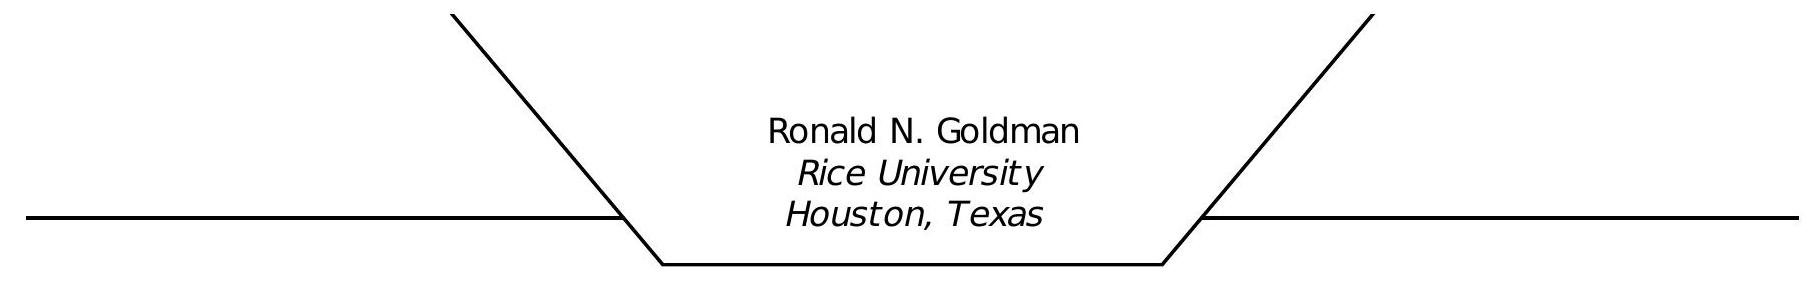
\includegraphics[max width=\textwidth]{2022_11_30_0cbb01a33d99487fc27fg-140}
\end{center}

Goal

Every nonsingular linear transformation of three-dimensional space is the product of three scales, two shears, and one rotation. The goal of this Gem is to show how to decompose any arbitrary, singular or nonsingular, linear or affine transformation of three-dimensional space into simple, geometrically meaningful, factors. For an alternative approach to similar problems (see Thomas, 1991).

\section{Nonsingular Linear Transformations}
Linear transformations of three-dimensional space are generally represented by $3 \times 3$ matrices. To decompose an arbitrary nonsingular linear transformation, consider, then, an arbitrary nonsingular $3 \times 3$ matrix L. We shall show that L can be factored into the product of three scales, two shears, and one rotation matrix.

Let the rows of L be given by the vectors $u, v$, w. Since the matrix L is nonsingular, the vectors $\mathrm{u}, \mathrm{v}, \mathrm{w}$ are linearly independent. Therefore, using the Gram-Schmidt orthogonalization procedure, we can generate 3 orthonormal vectors $u^{*}, v^{*}, w^{*}$ by setting

$$
\begin{aligned}
&\mathrm{u}^{*}=\mathrm{u} /|\mathrm{u}|, \\
&\mathrm{v}^{*}=\left(\mathrm{v}-\left(\mathrm{v} \cdot \mathrm{u}^{*}\right) \mathrm{u}^{*}\right) /\left|\mathrm{v}-\left(\mathrm{v} \cdot \mathrm{u}^{*}\right) \mathrm{u}^{*}\right|, \\
&\mathrm{w}^{*}=\left(\mathrm{w}-\left(\mathrm{w} \cdot \mathrm{u}^{*}\right) \mathrm{u}^{*}-\left(\mathrm{w} \cdot \mathrm{v}^{*}\right) \mathrm{v}^{*}\right) /\left|\mathrm{w}-\left(\mathrm{w} \cdot \mathrm{u}^{*}\right) \mathrm{u}^{*}-\left(\mathrm{w} \cdot \mathrm{v}^{*}\right) \mathrm{v}^{*}\right| .
\end{aligned}
$$

GRAPHICS GEMS III Edited by DAVID KIRK This orthogonalization procedure can be used to decompose the matrix L into the desired factors.

Begin with the rotation. By construction, the matrix $R$ whose rows are $u^{*}, v^{*}, w^{*}$ is an orthogonal matrix. If $\operatorname{Det}(R)=-1$, replace $w^{*}$ by $-w^{*}$. Then $R$ is the rotation matrix we seek. Using the results in Goldman (1991a), we can, if we like, retrieve the rotation axis and angle from the matrix R.

The three scaling transformations are also easy to find. Let

$$
\begin{aligned}
&\mathrm{s}_{1}=|\mathrm{u}|, \\
&\mathrm{s}_{2}=\left|\mathrm{v}-\left(\mathrm{v} \cdot \mathrm{u}^{*}\right) \mathrm{u}^{*}\right|, \\
&\mathrm{s}_{3}=\left|\mathrm{w}-\left(\mathrm{w} \cdot \mathrm{u}^{*}\right) \mathrm{u}^{*}-\left(\mathrm{w} \cdot \mathrm{v}^{*}\right) \mathrm{v}^{*}\right| .
\end{aligned}
$$

That is, $s_{1}, s_{2}, s_{3}$ are the lengths of $u^{*}, v^{*}, w^{*}$ before they are normalized. Now let $\mathrm{S}$ be the matrix with $\mathrm{s}_{1}, \mathrm{~s}_{2}, \mathrm{~s}_{3}$ along the diagonal and with zeroes everywhere else. The matrix $\mathrm{S}$ represents the three independent scaling transformations that scale by $s_{1}$ along the $x$-axis, $s_{2}$ along the $y$-axis, and $s_{3}$ along the z-axis. (If $\operatorname{Det}(R)$ was originally $-1$, then replace $s_{3}$ by $-s_{3}$. In effect, this mirrors points in the xy-plane.)

Before we can introduce the two shears, we need to recall notation for the identity matrix and the tensor product of two vectors.

Identity:

$$
I=\left|\begin{array}{lll}
1 & 0 & 0 \\
0 & 1 & 0 \\
0 & 0 & 1
\end{array}\right|
$$

\section{Tensor Product:}
$$
\nu \otimes \omega=\left|\begin{array}{lll}
v_{1} \omega_{1} & v_{1} \omega_{2} & v_{1} \omega_{3} \\
v_{2} \omega_{1} & v_{2} \omega_{2} & v_{2} \omega_{3} \\
v_{3} \omega_{1} & v_{3} \omega_{2} & v_{3} \omega_{3}
\end{array}\right|=\left|\begin{array}{l}
v_{1} \\
v_{2} \\
v_{3}
\end{array}\right| *\left|\omega_{1} \omega_{2} \omega_{3}\right|=v^{\mathrm{t}} * \omega .
$$

Here $*$ denotes matrix multiplication and the superscript $\mathrm{t}$ denotes

\section{III.3 DECOMPOSING LINEAR AND AFFINE TRANSFORMATIONS}
transpose. Observe that for all vectors $\mu$

$$
\begin{gathered}
\mu \cdot \mathrm{I}=\mu, \\
\mu *(\nu \otimes \omega)=(\mu \cdot v) \omega .
\end{gathered}
$$

Now we are ready to define the two shears. Recall from Goldman (199lb) that a shear $\mathrm{H}$ is defined in terms of a unit vector $\mathrm{v}$ normal to a plane $Q$, a unit vector $\omega$ in the plane $Q$, and an angle $\varphi$ by setting

$$
\mathrm{H}=\mathrm{I}+\tan \varphi(v \otimes \omega) .
$$

Let $\mathrm{H}_{1}$ be the shear defined by unit normal $v^{*}$, the unit vector $\mathrm{u}^{*}$, and the angle $\theta$ by setting

$$
\begin{aligned}
&\mathrm{H}_{1}=\mathrm{I}+\tan \theta\left(\mathrm{v}^{*} \otimes \omega^{*}\right), \\
&\tan \theta=\mathrm{v} \cdot \mathrm{u}^{*} / \mathrm{s}_{2} .
\end{aligned}
$$

Similarly, let $\mathrm{H}_{2}$ be the shear defined by unit normal $\mathrm{w}^{*}$, the unit vector $r^{*}$, and the angle $\psi$ by setting

$$
\begin{gathered}
\mathrm{H}_{2}=\mathrm{I}+\tan \psi\left(\mathrm{w}^{*} \otimes \mathrm{r}^{*}\right), \\
\tan \psi=\operatorname{SQRT}\left\{\left(\mathrm{w} \cdot \mathrm{u}^{*}\right)^{2}+\left(\mathrm{w} \cdot \mathrm{v}^{*}\right)^{2}\right\} / \mathrm{s}_{3^{\prime}} \\
\mathrm{r}^{*}=\left\{\left(\mathrm{w} \cdot \mathrm{u}^{*}\right) \mathrm{u}^{*}+\left(\mathrm{w} \cdot \mathrm{v}^{*}\right) \mathrm{v}^{*}\right\} \mathrm{s}_{3} \tan \psi
\end{gathered}
$$

Then it is easy to verify that

$$
\begin{aligned}
&\mathrm{u}^{*} * \mathrm{H}_{1}=\mathrm{u}^{*}, \quad \mathrm{v}^{*} * \mathrm{H}_{1}=\mathrm{v}^{*}+\left(\mathrm{v} \cdot \mathrm{u}^{*} / \mathrm{s}_{2}\right) \mathrm{u}^{*}, \quad \mathrm{w}^{*} * \mathrm{H}_{1}=\mathrm{w}^{*}, \\
&\mathrm{u}^{*} * \mathrm{H}_{2}=\mathrm{u}^{*}, \quad \mathrm{v}^{*} * \mathrm{H}_{2}=\mathrm{v}^{*}, \\
&\mathrm{w}^{*} * \mathrm{H}_{2}=\mathrm{w}^{*}+\left\{\left(\mathrm{w} \cdot \mathrm{u}^{*}\right) \mathrm{u}^{*}+\left(\mathrm{w} \cdot \mathrm{v}^{*}\right) \mathrm{v}^{*}\right\} / \mathrm{s}_{3} .
\end{aligned}
$$

Finally, we shall show that

$$
\mathrm{L}=\mathrm{S} * \mathrm{R} * \mathrm{H}_{1} * \mathrm{H}_{2}
$$

Since the transformation L is linear, we need only check that both sides give the same result on the canonical basis $\mathbf{i}, \mathbf{j}, \mathbf{k}$. By construction we know that

$$
\mathbf{i} * \mathrm{~L}=\mathrm{u}, \quad \mathbf{j} * \mathrm{~L}=\mathrm{v}, \quad \mathbf{k} * \mathrm{~L}=\mathrm{w},
$$

so we need to verify that we get the same results for the right-hand side. Let us check.

First,

$$
\begin{aligned}
\mathbf{i} * \mathrm{~S} * \mathrm{R} * \mathrm{H}_{1} * \mathrm{H}_{2} &=\left(\mathrm{s}_{1}\right) \mathbf{i} * \mathrm{R} * \mathrm{H}_{1} * \mathrm{H}_{2} \\
&=\left(\mathrm{s}_{1}\right) \mathrm{u}^{*} * \mathrm{H}_{1} * \mathrm{H}_{2} \\
&=\mathrm{u} .
\end{aligned}
$$

since by construction the two shears $\mathrm{H}_{1}$ and $\mathrm{H}_{2}$ do not affect $\mathrm{u}^{*}$. Next,

$$
\begin{aligned}
\mathbf{j} * \mathrm{~S} * \mathrm{R} * \mathrm{H}_{1} * \mathrm{H}_{2} &=\left(\mathrm{s}_{2}\right) \mathbf{j} * \mathrm{R} * \mathrm{H}_{1} * \mathrm{H}_{2} \\
&=\left(\mathrm{s}_{2}\right) \mathrm{v}^{*} * \mathrm{H}_{1} * \mathrm{H}_{2} \\
&=\left\{\mathrm{s}_{2} \mathrm{v}^{*}+\left(\mathrm{v} \cdot \mathrm{u}^{*}\right) \mathrm{u}^{*}\right\} * \mathrm{H}_{2} \\
&=\mathrm{s}_{2} \mathrm{v}^{*}+\left(\mathrm{v} \cdot \mathrm{u}^{*}\right) \mathrm{u}^{*} \\
&=\mathrm{v} .
\end{aligned}
$$

Finally,

$$
\begin{aligned}
\mathbf{k} * \mathrm{~S} * \mathrm{R} * \mathrm{H}_{1} * \mathrm{H}_{2} &=\left(\mathrm{s}_{3}\right) \mathbf{k} * \mathrm{R} * \mathrm{H}_{1} * \mathrm{H}_{2} \\
&=\left(\mathrm{s}_{3}\right) \mathrm{w}^{*} * \mathrm{H}_{1} * \mathrm{H}_{2} \\
&=\left(\mathrm{s}_{3}\right) \mathrm{w}^{*} * \mathrm{H}_{2} \\
&=\mathrm{s}_{3} \mathrm{w}^{*}+\left(\mathrm{w} \cdot \mathrm{u}^{*}\right) \mathrm{u}^{*}+\left(\mathrm{w} \cdot \mathrm{v}^{*}\right) \mathrm{v}^{*} \\
&=\mathrm{w} .
\end{aligned}
$$

\section{III.3 DECOMPOSING LINEAR AND AFFINE TRANSFORMATIONS}
Although we have succeeded in factoring an arbitrary nonsingular linear transformation, notice that this decomposition is not unique. Indeed, the Gram-Schmidt orthogonalization procedure depends upon the ordering of the vectors to which it is applied. We could, for example, have applied the Gram-Schmidt procedure to the vectors in the order w, u, v instead of $u, v$, w. We would then have retrieved a different decomposition of the same matrix. Nevertheless, this procedure is still of some value since it allows us to decompose an arbitrary nonsingular linear transformation into simple, geometrically meaningful factors.

\section{Singular Linear Transformations}
Now let L be an arbitrary singular $3 \times 3$ matrix. There are three cases to consider, depending on the rank of L. If $\operatorname{rank}(\mathrm{L})=0$, there is nothing to do since L simply maps all vectors into the zero vector. The case $\operatorname{rank}(\mathrm{L})=1$ is also essentially trivial, since all vectors are simply appropriately scaled and then projected onto a single fixed vector. Therefore, we shall concentrate on the case where $\operatorname{rank}(\mathrm{L})=2$.

We will show that when $\operatorname{rank}(\mathrm{L})=2$, we still need one rotation, but we require only two scales, one shear, and one parallel projection. Thus, the number of scales is reduced by one and a shear is replaced by a parallel projection. Moreover, we shall shovv that the parallel projection can be replaced by a shear followed by an orthogonal projection.

Again, let the rows of L be given by the vectors $u, v$, w. Since the matrix $L$ is singular, the row vectors $u, v, w$ are linearly dependent, but since $\operatorname{rank}(\mathrm{L})=2$, two rows of $\mathrm{L}$ are linearly independent. For simplicity and without loss of generality, we will assume that $u$ and $v$ are linearly independent.

Modifying the Gram-Schmidt orthogonalization procedure, we can generate three orthonormal vectors $u^{*}, v^{*}, w^{*}$ by setting

$$
\begin{aligned}
u^{*} &=u /|u|, \\
v^{*} &=\left(v-\left(v \cdot u^{*}\right) u^{*}\right) /\left|v-\left(v \cdot u^{*}\right) u^{*}\right|, \\
w^{*} &=u^{*} \times v^{*} .
\end{aligned}
$$

This orthogonalization procedure can again be used to decompose the matrix L into the desired factors.

By construction, the matrix $R$ whose rows are $u^{*}, v^{*}, w^{*}$ is an orthogonal matrix and $\operatorname{Det}(\mathrm{R})=1$. The matrix $\mathrm{R}$ is the rotation matrix that we seek. We can recover the axis and angle of rotation from the matrix $\mathrm{R}$ using the techniques described in Goldman (199la).

The two scaling transformations are also easy to find. Let

$$
\begin{aligned}
&\mathrm{s}_{1}=|\mathrm{u}|, \\
&\mathrm{s}_{2}=\left|\mathrm{v}-\left(\mathrm{v} \cdot \mathrm{u}^{*}\right) \mathrm{u}^{*}\right| .
\end{aligned}
$$

Note that $s_{1}, s_{2}$ are, respectively, the lengths of $u^{*}, v^{*}$ before they are normalized. Now let $\mathrm{S}$ be the matrix with $\mathrm{s}_{1}, \mathrm{~s}_{2}, 1$ along the diagonal and with zeroes everywhere else. The matrix $S$ represents the two independent scaling transformations that scale by $\mathrm{s}_{1}$ along the $\mathrm{x}$-axis and $\mathrm{s}_{2}$ along the y-axis.

The shear $\mathrm{H}$ is the same as the first of the two shears that we used to decompose a nonsingular linear transformation. Using the notation for the identity matrix and the tensor product of two vectors that we established above,

$$
\begin{aligned}
\mathrm{H} &=\mathrm{I}+\tan \theta\left(\mathrm{v}^{*} \otimes \mathrm{u}^{*}\right), \\
\tan \theta &=\mathrm{v} \cdot \mathrm{u}^{*} / \mathrm{s}_{2} .
\end{aligned}
$$

Thus, $\mathrm{H}$ is the shear defined by the unit normal vector $\mathrm{v}^{*}$, the unit vector $u^{*}$, and the angle $\theta$. Again, it is easy to verify that

$$
u^{*} * H=u^{*}, \quad v^{*} * H=v^{*}+\left(v \cdot u^{*} / s_{2}\right) u^{*}, \quad w^{*} * H=w^{*} .
$$

Last, we define the parallel projection $P$ to be projection into the $u^{*} v^{*}$-plane parallel to the vector( $\left.w^{*}-\mathrm{w}\right)$. According to Goldman(1990), the matrix $\mathrm{P}$ is given by

$$
\mathrm{P}=\mathrm{I}-\mathrm{w}^{*} \otimes\left(\mathrm{w}^{*}-\mathrm{w}\right)
$$

Notice that if $\mathrm{w}=0$, this parallel projection reduces to orthogonal projection into the $u^{*} v^{*}$-plane (Goldman, 1990). In any event, it is easy

\section{III.3 DECOMPOSING LINEAR AND AFFINE TRANSFORMATIONS}
to verify that

$$
\mathrm{u}^{*} * \mathrm{P}=\mathrm{u}^{*}, \quad \mathrm{v}^{*} * \mathrm{P}=\mathrm{v}^{*}, \quad \mathrm{w}^{*} * \mathrm{P}=\mathrm{w} .
$$

Finally, let us show that

$$
\mathrm{L}=\mathrm{S} * \mathrm{R} * \mathrm{H} * \mathrm{P}
$$

by checking that both sides give the same result on the canonical basis $\mathbf{i}, \mathbf{j}$, k. By construction we know that

$$
\mathbf{i} * \mathrm{~L}=\mathrm{u}, \quad \mathbf{j} * \mathrm{~L}=\mathrm{v}, \quad \mathbf{k} * \mathrm{~L}=\mathrm{w},
$$

so we need to verify that we get the same results for the right-hand side. Let us check.

First,

$$
\begin{aligned}
\mathbf{i} * \mathrm{~S} * \mathrm{R} * \mathrm{H} * \mathrm{P} &=\left(\mathrm{s}_{1}\right) \mathbf{i} * \mathrm{R} * \mathrm{H} * \mathrm{P} \\
&=\left(\mathrm{s}_{1}\right) \mathrm{u}^{*} * \mathrm{H} * \mathrm{P} \\
&=\mathrm{s}_{1} \mathrm{u}^{*} \\
&=\mathrm{u},
\end{aligned}
$$

since by construction the two linear transformations $\mathrm{H}$ and $\mathrm{P}$ do not affect $u^{*}$.

Next,

$$
\begin{aligned}
\mathbf{j} * \mathrm{~S} * \mathrm{R} * \mathrm{H} * \mathrm{P} &=\left(\mathrm{s}_{2}\right) \mathbf{j} * \mathrm{R} * \mathrm{H} * \mathrm{P} \\
&=\left(\mathrm{s}_{2}\right) \mathrm{v}^{*} * \mathrm{H} * \mathrm{P} \\
&=\left\{\mathrm{s}_{2} \mathrm{v}^{*}+\left(\mathrm{v} \cdot \mathrm{u}^{*}\right) \mathrm{u}^{*}\right\} * \mathrm{P} \\
&=\mathrm{s}_{2} \mathrm{v}^{*}+\left(\mathrm{v} \cdot \mathrm{u}^{*}\right) \mathrm{u}^{*} \\
&=\mathrm{v} .
\end{aligned}
$$

\section{III.3 DECOMPOSING LINEAR AND AFFINE TRANSFORMATIONS}
Finally,

$$
\begin{aligned}
\mathbf{k} * \mathrm{~S} * \mathrm{R} * \mathrm{H} * \mathrm{P} &=\mathbf{k} * \mathrm{R} * \mathrm{H} * \mathrm{P} \\
&=\mathrm{w}^{*} * \mathrm{H} * \mathrm{P} \\
&=\mathrm{w}^{*} * \mathrm{P} \\
&=\mathrm{w} .
\end{aligned}
$$

By the way, every parallel projection can be written as the product of a shear followed by an orthogonal projection. To see this, recall that a projection $P$ parallel to the vector $\omega$ into the plane with normal vector $n$ is given by Goldman (1990):

$$
P=I-(n \otimes \omega) / n \cdot \omega .
$$

Consider the orthogonal projection 0 into the plane perpendicular to the unit vector $n$ (Goldman, 1990),

$$
0=I-(n \otimes n),
$$

and the shear $\mathrm{K}$ defined by the unit normal vector $\mathrm{n}$, the unit vector $v=(\mathrm{n}-\omega / \omega \cdot \mathrm{n}) /|\mathrm{n}-\omega / \omega \cdot \mathrm{n}|$, and the angle $\theta$ given by $\tan \theta=$ $|\mathrm{n}-\omega / \omega \cdot \mathrm{n}|:$

$$
K=I+\tan \theta(n \otimes \nu) .
$$

Since $v \cdot \mathrm{n}=0$, it follows that $(\mathrm{n} \otimes v) *(\mathrm{n} \otimes \mathrm{n})=(v \cdot \mathrm{n})(\mathrm{n} \otimes \mathrm{n})=0$. Therefore,

$$
I-(n \otimes \omega) / n \cdot \omega=\{1+\tan \theta(n \otimes \nu)\} *\{I-(n \otimes n)\},
$$

or, equivalently,

$$
\mathrm{P}=\mathrm{K} * 0
$$

In our case $\omega=\mathrm{w}^{*}-\mathrm{w}, \mathrm{n}=\mathrm{w}^{*}$, and $v=\mathrm{w}$. Thus, we have shown that when $\operatorname{rank}(\mathrm{L})=2$, we can factor L into the product of two scales one rotation, two shears, and one orthogonal projection. This decomposition is the same as in the nonsingular case, except that the number of scales is reduced by one and the standard nonsingular factors-scales, rotation, and shears-are followed by an orthogonal projection.

\section{III.3 DECOMPOSING LINEAR AND AFFINE TRANSFORMATIONS}
Notice again that this decomposition is not unique. Indeed, the modified Gram-Schmidt orthogonalization procedure also depends upon the ordering of the vectors to which it is applied. We could, for example, have applied the Gram-Schmidt procedures to the vectors in the order $v$, u instead of $u$, v. We would then have retrieved a different decomposition of the same matrix. Nevertheless, this procedure is still of some value since it allows us to decompose an arbitrary singular linear transformation into simple, geometrically meaningful factors.

\section{Affine Transformations}
Finally, recall that every affine transformation A is simply a linear transformation $\mathrm{L}$ followed by a translation $\mathrm{T}$. If the affine transformation is represented by a $4 \times 3$ matrix

$$
\mathrm{A}=\left|\begin{array}{l}
\mathrm{L} \\
\mathrm{T}
\end{array}\right|,
$$

then the upper $3 \times 3$ submatrix L represents the linear transformation and the fourth row $\mathrm{T}$ represents the translation vector. Thus, to decompose an arbitrary affine transformation into simpler, geometrically meaningful factors, simply factor the associated linear transformation L and append the translation T. Thus, every nonsingular affine transformation of three-dimensional space can be factored into the product of three scales, two shears, one rotation, and one translation. Similarly, every singular affine transformation of three-dimensional space can be factored into the product of two scales, two shears, one rotation, one orthogonal projection, and one translation. Again, these decompositions are not unique, since the decompositions of the associated linear transformations are not unique. Nevertheless, these procedures are still of some value since they allow us to decompose arbitrary affine transformations into simple, geometrically meaningful factors.

See also G2, 319; G2, 320; G3, C.2.\\
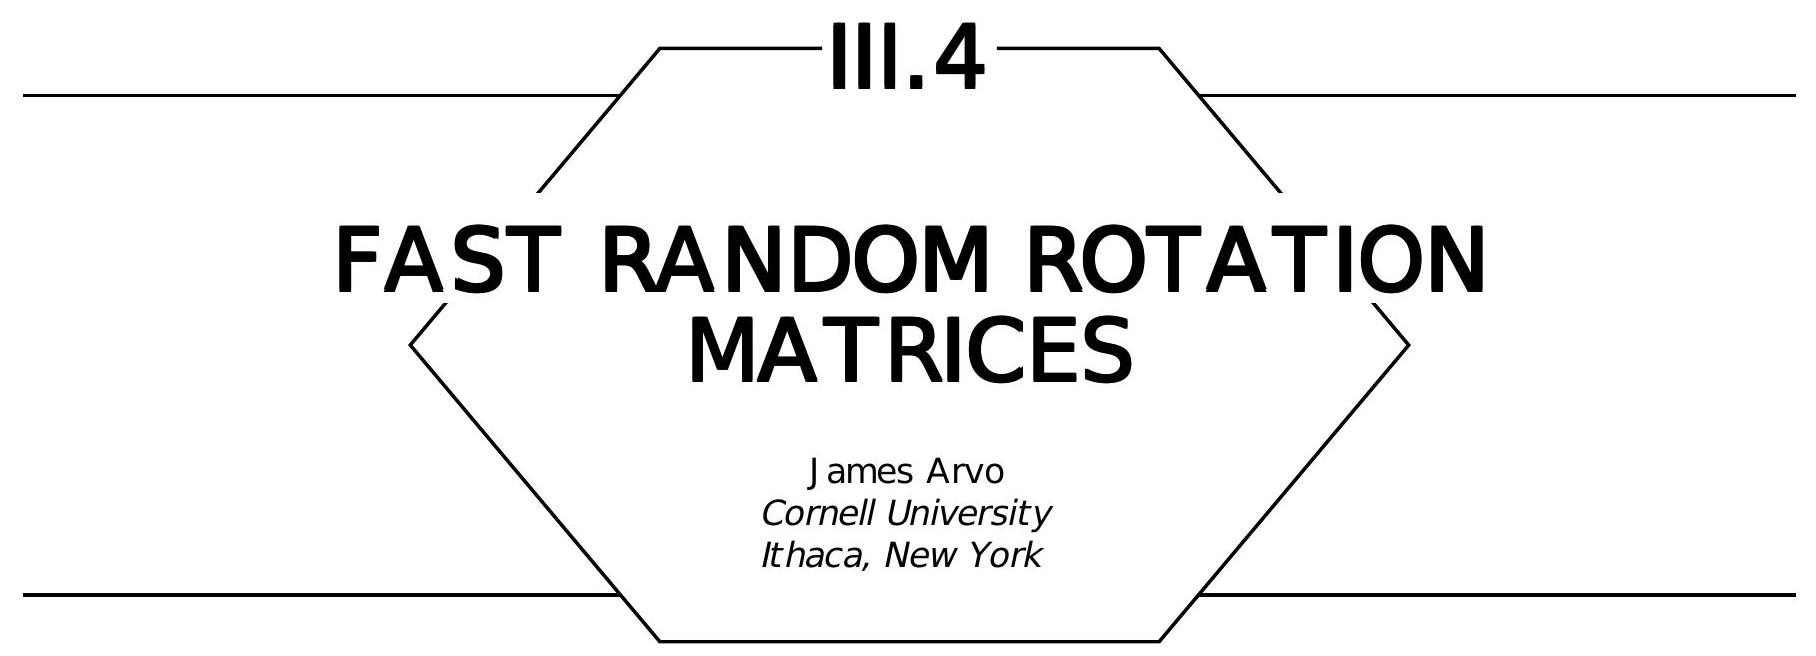
\includegraphics[max width=\textwidth, center]{2022_11_30_0cbb01a33d99487fc27fg-149}

In a previous Gem (Arvo, 1991), I described a method for generating random rotation matrices based on random unit quaternions. As Ken Shoemake points out in his Gem (III.6) that algorithm was flawed in that it did not generate uniformly distributed rotation matrices. For a method based on quaternions that corrects this defect see his algorithm. In this Gem I describe a completely different approach to solving the same problem that has the additional benefit of being slightly faster than the previous method. The approach is based on the following fact:

To generate uniformly distributed random rotations of a unit sphere, first perform a random rotation about the vertical axis, then rotate the north pole to a random position.

The first step of this prescription is trivial. Given a random number, $\mathrm{x}_{1}$, between 0 and 1. the matrix $\mathrm{R}$ does the trick:

$$
R=\begin{array}{ccc}
\cos \left(2 \pi \mathrm{x}_{1}\right) & \sin \left(2 \pi \mathrm{x}_{1}\right) & 0 \\
-\sin \left(2 \pi \mathrm{x}_{1}\right) & \cos \left(2 \pi \mathrm{x}_{1}\right) & 0 \\
0 & 0 & 1
\end{array} .
$$

Here we are assuming that the z-axis is the vertical axis, so the "north pole" will be the point $\mathrm{z}=(0,0,1)$. The second operation is not quite so obvious, but fortunately it can be carried out quite efficiently. Observe that we can take the point $\mathrm{z}$ to any other point $\mathrm{p}$ on the sphere via a

\section{III.4 FAST RANDOM ROTATION MATRICES}
reflection through the plane orthogonal to the line $\overline{\mathrm{zp}}$ and containing the origin. Such a reflection is given by the Householder matrix

$$
H=I-2 v^{T},
$$

where $\mathrm{v}$ is a unit vector parallel to $\overline{\mathrm{zp}}$ (see, for instance, Golub and Van Loan, 1985). To turn this into a rotation we need only apply one more reflection (making the determinant positive). A convenient reflection for this purpose is reflection through the origin-that is, scaling by $-1$. Thus, the final rotation matrix can be expressed as the product

$$
M=-H R,
$$

where $R$ is the simple rotation in Eq. (1). The rotation matrix M will be uniformly distributed within $\mathrm{SO}(3)$, the set of all rotations in three-space, if $\mathrm{H}$ takes the north pole to every point on the sphere with equal probability density. This will hold if the image of z under the random reflection is such that both its azimuth angle and the cosine of its elevation angle are uniformly distributed. The matrix $\mathrm{H}$ in Eq. (2) will satisfy these requirements if we let

$$
\mathrm{v}=\begin{gathered}
\cos \left(2 \pi \mathrm{x}_{2}\right) \sqrt{\mathrm{x}_{3}} \\
\sin \left(2 \pi \mathrm{x}_{2}\right) \sqrt{\mathrm{x}_{3}} \\
\sqrt{1-\mathrm{x}_{3}}
\end{gathered},
$$

where $x_{2}$ and $x_{3}$ are two independent uniform random variables in $[0,1]$. To show this we need only compute $p=H z$ and verify that $p$ is distributed appropriately. Using the preceding definition of $\mathrm{v}$, we have

$$
p=z-2 v^{T} z=\begin{gathered}
-2 \cos \left(2 \pi x_{2}\right) \sqrt{x_{3}\left(1-\mathrm{x}_{3}\right)} \\
-2 \sin \left(2 \pi x_{2}\right) \sqrt{x_{3}\left(1-\mathrm{x}_{3}\right)} \\
2 \mathrm{x}_{3}-1
\end{gathered} .
$$

Because the third component of $p$ is the cosine of its elevation angle, we see immediately that it is uniformly distributed over $[-1,1]$, as required.

\section{III.4 FAST RANDOM ROTATION MATRICES}
random\_rotation $\left(x_{1}, x_{2}, x_{2}, M\right)$

$x_{1}, x_{2}, x_{3}$ : real; Three random variables.

$M$ : matrix3; The resulting matrix.

begin

$\theta \leftarrow 2 \pi x_{1} ; \quad$ Pick a rotation about the pole.

$\phi \leftarrow 2 \pi x_{2} ; \quad$ Pick a direction to deflect the pole.

$z \leftarrow x_{3} ; \quad$ Pick the amount of pole deflection.

Construct a vector for performing the reflection.

$V \leftarrow\left[\begin{array}{c}\cos \phi \sqrt{z} \\ \sin \phi \sqrt{z} \\ \sqrt{1-z}\end{array}\right]$

Construct the rotation matrix by combining two

simple rotations: first rotate about the $Z$ axis,

then rotate the $Z$ axis to a random orientation.

$M \leftarrow\left(2 V V^{\mathrm{T}}-I\right)\left[\begin{array}{ccc}\cos \theta & \sin \theta & 0 \\ -\sin \theta & \cos \theta & 0 \\ 0 & 0 & 1\end{array}\right]$

end

Figure 1. An efficient procedure for creating random $3 \times 3$ rotation matrices.

Similarly, from its first two components we see that the azimuth angle of $p$ is $2 \pi x_{2}$, which is uniformly distributed over $[0,2 \pi]$.

The complete algorithm combining the reflection and simple rotation is shown in Fig. 1, and an optimized version in C appears in the appendix. Procedure "random\_rotation" requires three uniformly distributed random numbers between 0 and 1. Supplying these values as arguments has several advantages. First, the procedure can be used in conjunction with your favorite pseudorandom number generator, and there are a great many to choose from. Secondly, if we obtain the three random numbers by stratified or jittered sampling of the unit cube, the resulting rotation

\section{III.4 FAST RANDOM ROTATION MATRICES}
\begin{center}
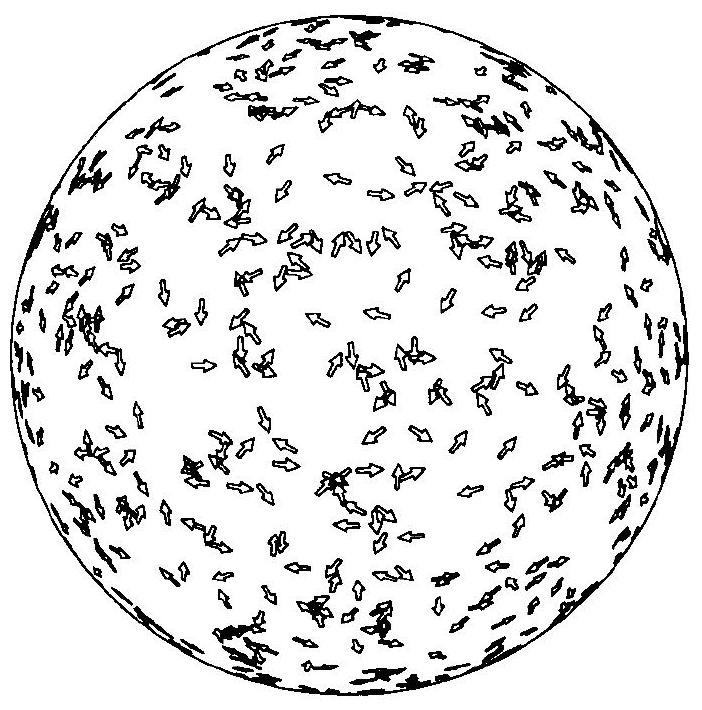
\includegraphics[max width=\textwidth]{2022_11_30_0cbb01a33d99487fc27fg-152}
\end{center}

(a)

\begin{center}
\includegraphics[max width=\textwidth]{2022_11_30_0cbb01a33d99487fc27fg-152(1)}
\end{center}

(b)

Figure 2.

matrices will inherit the benefits-namely, less clumping. Finally, if we restrict the range of the random input variables (while maintaining their uniformity), we can generate uniformly distributed perturbations or "wobbles" within given limits.

Figure $2 \mathrm{a}$ shows the result of applying 1,000 random rotations to a sphere with an arrow painted at one pole. The resulting pattern looks much the same from any vantage point, providing visual confirmation of uniformity. Figure $2 \mathrm{~b}$ was generated by restricting $\mathrm{x}_{1}$ and $\mathrm{x}_{3}$ to the range $[0,0.1]$

See also G2, 355; G3, C.6.

\begin{center}
\includegraphics[max width=\textwidth]{2022_11_30_0cbb01a33d99487fc27fg-153}
\end{center}

\section{Introduction}
Spencer, (1991) explains how to express a matrix as a set of parameters, called an unmatrix. In Spencer's unmatrix, each parameter is a single value that can be interpolated using linear interpolation or piecewise splining techniques. When simple interpolation is used to calculate transformations between samples, unnatural motion can occur.

This Gem shows how to interpolate motion naturally between two sample matrices for use in motion control or key-framing applications. This technique was used to create the key frame animation system described in Dana (1991).

\section{Interpolating in Logarithmic Space}
Unnatural or accelerated motion occurs when scaling parameters are interpolated in a straightforward way. A simple interpolation, halfway between a scaling parameter of $0.50$ and 2.0, produces a value of $1.25$ when the visually expected value would be 1.0.

A solution to this problem is to interpolate the logarithm of the scaling parameter.

\section{III.5 ISSUES AND TECHNIQUES FOR KEYFRAMING TRANSFORMATIONS}
\section{Relative Motion}
The most natural motion from one sample transformation to another is the one that takes the shortest apparent path. When rotation parameters are interpolated, sometimes the shortest path may cross the zero degree mark. For example, the shortest path between 10 degrees and 350 degrees is $-20$ degrees, not $+340$ degrees.

A second rotation problem occurs when you want an object to appear to rotate relative to its own oriental ion instead of relative to its current orientation in the 3-D universe.

To get the desired transformation and to solve both the zero mark problem and the axis problem:

\begin{enumerate}
  \item Express the motion between two samples relative to the first sample, prior to interpolation.

  \item Calculate the interpolation using an identity transformation and the difference between the two samples.

  \item Concatenate the interpolated transformation to the first sample.

\end{enumerate}

This solves the zero mark problem because the rotational values of an identity transformation are all zero. It also solves the axis problem by expressing a segment of motion relative to the segment's first sample.

\section{Linear vs. Splined Interpolation}
Although it might seem best to use a splining technique to interpolate all the parameters of an unmatrix, experience has shown that ordinary linear interpolation is best for the scaling, shearing, rotation, and perspective parameters, and splined interpolation is best for the translation parameters.

\section{III.5 ISSUES AND TECHNIQUES FOR KEYFRAMING TRANSFORMATIONS}
\section{Subdividing Motion}
For a motion to have constant speed between two samples, the motion must be subdivided into intervals of equal length in space, not just duration in time. When using splined interpolation to interpolate translation parameters, the spline type must allow for even subdivision along the length of a piece. A spline, such as a Cardinal spline, should be used.

See also G3, C.7.\\
\includegraphics[max width=\textwidth, center]{2022_11_30_0cbb01a33d99487fc27fg-156}

\section{Background}
A previous Graphics Gem (Arvo, 1991) presented an algorithm for generating random rotations, in both quaternion and matrix form. It takes as input three uniform deviates and efficiently computes a random rotation with a uniformly distributed axis and a uniformly distributed angle. The purpose of the present gem is to demonstrate that, surprisingly, that algorithm does not generate a uniformly distributed rotation, and to give two simple algorithms that do.

How can the distribution of the axis and angle be uniform, and yet the distribution of the rotations not be? To answer that question requires, first of all, a definition of uniformity. Since rotations form a group, an approach that is both standard and intuitively satisfying uses "Haar measure" as follows: If $\mathrm{X}$ is a random rotation with uniform distribution, then for any fixed but arbitrary rotation R, RX and XR have the same distribution as $X$. A rough physical analogy is the testing of a bicycle wheel for balance by spinning it and looking for wobbles, or dragging a flat edge across freshly poured cement to smooth it.

\section{Planar Rotations}
Before examining the implications of this definition for spatial rotations, let us first examine its application to the simpler case of planar rotations, where we can use both our eyes and our intuition. A planar rotation can be represented in several ways, for example as an angle between 0 and

\section{III.6 UNIFORM RANDOM ROTATIONS}
$2 \pi$, as a unit complex number $\mathrm{x}+\mathbf{i} \mathrm{y}=\cos \theta+\mathbf{i} \sin \theta$, and as a matrix

\begin{center}
\includegraphics[max width=\textwidth]{2022_11_30_0cbb01a33d99487fc27fg-157}
\end{center}

Planar rotations combine by summing their angles modulo $2 \pi$, so one way to generate a uniform planar rotation is to generate a uniform angle. Combination of $\mathrm{X}$ with $\mathrm{R}$ merely slides the angle around. Since this leaves the distribution unchanged, it is uniform. A more geometrical interpretation of this problem is that we want to generate points uniformly distributed on the unit circle $x^{2}+y^{2}=1$, with probability proportional to arc length. Note that the average magnitude of $x$ will be $1 / \pi$ times the integral of $2 \cos \theta$ from 0 to $\pi / 2$, namely $2 / \pi \approx 0.6366$. This computation is merely "summing"-integrating-the $\mathrm{x}$ values of all the points on the right half of the circle and dividing by the "number of points" used-the arc length of that half of the circle. Here and subsequently we take advantage of circle (later, sphere) and sinusoid symmetries when computing magnitudes. Now suppose a rotation is generated by choosing a uniformly distributed $\mathrm{x}$ between $-1$ and $+1$, with $\mathrm{y}$

\begin{center}
\includegraphics[max width=\textwidth]{2022_11_30_0cbb01a33d99487fc27fg-157(1)}
\end{center}

Figure 1. Haar test reveals distribution lumps.

\section{III.6 UNIFORM RANDOM ROTATIONS}
computed as $\pm \sqrt{1-x^{2}}$ (either sign being equally likely). For this distribution the average magnitude of $\mathrm{x}$ will be $\frac{1}{2}$, and so it cannot give uniformly distributed rotations.

\section{Uniform Spherical Distribution}
Shortly, we are going to want to know about points uniformly distributed on a sphere, and on a hypersphere. The sphere case is easier to visualize, and has a surprising result: Each coordinate of a point uniformly distributed on a sphere is uniformly distributed! Thus, for example, the average magnitude of the $x$ coordinate is $\frac{1}{2}$. A uniformly distributed point can be generated by choosing $z$ uniformly distributed on $-1$ to $+1$, and $\mathrm{x}$ and $\mathrm{y}$ uniformly distributed on a circle of radius $\sqrt{1-\mathrm{z}^{2}}$, a fact exploited in Arvo's algorithm (Arvo, 1991).

To derive the $\mathrm{x}$ distribution and average magnitude, we integrate circular slices. Since the sphere is symmetrical, and only positive $\mathrm{x}$ values lie in the right hemisphere, we will confine our attention there.

\begin{center}
\includegraphics[max width=\textwidth]{2022_11_30_0cbb01a33d99487fc27fg-158}
\end{center}

Figure 2. Density and average of $\mathrm{x}$ for planar rotation.

\section{III.6 UNIFORM RANDOM ROTATIONS}
Calculation will be simpler if the variable of integration is $\theta$, with $\mathrm{x}=\sin \theta$; then the radius of the circular slice at $\mathrm{x}$ will be $\cos \theta$, and its perimeter length $2 \pi \cos \theta$. The area of the hemisphere is, of course, just the integral of the perimeters for $\theta$ from 0 to $\pi / 2$, which is $2 \pi$. For the circle, the integral for average magnitude weighted each $\mathrm{x}$ value by 2 , since the one-dimensional slices gave exactly two points. Now the weight for $\mathrm{x}=\sin \theta$ will be $2 \pi \cos \theta$, because of the circular slice. (There, $\mathrm{x}$ was $\cos \theta$; here, $\sin \theta$.) So the average magnitude is

$$
\frac{1}{2 \pi} \int^{\pi / 2}-2 \pi \cos \theta \sin \theta \mathrm{d} \theta=\frac{1}{2} .
$$

To find the probability of a value being between 0 and $\mathrm{x}$, we simply integrate the circular slices from 0 to arcsin $\mathrm{x}$, giving

$$
\frac{1}{2 \pi} \int_{0}^{\arcsin x}-2 \pi \cos \theta \mathrm{d} \theta=\mathrm{x} \text {. }
$$

This shows that the coordinate distributions are uniform (though not independently so!) for points uniformly distributed on a sphere.

\begin{center}
\includegraphics[max width=\textwidth]{2022_11_30_0cbb01a33d99487fc27fg-159}
\end{center}

Figure 3. Sphere distribution integral.

\section{III.6 UNIFORM RANDOM ROTATIONS}
\section{Spatial Rotations}
With these warm-up exercises behind us, we are ready to tackle spatial rotations. Once again there are several possible representations, including Euler angles $\left(\theta_{x^{\prime}}, \theta_{y}, \theta_{z}\right)$, unit quaternions $\mathrm{w}+\mathbf{i v}+\mathbf{j x}+\mathbf{k z}$ (Shoemake, 1985, 1989), and $3 \times 3$ matrices

$$
\begin{array}{ccc}
1-2\left(y^{2}+z^{2}\right) & 2 x y-2 w z & 2 x z+2 w y \\
2 x y+2 w z & 1-2\left(x^{2}+z^{2}\right) & 2 y z-2 w x \\
2 x z-2 w y & 2 y z+2 w x & 1-2\left(x^{2}+y^{2}\right)
\end{array}
$$

In this case, unit quaternions are the best representation, and the geometric problem turns out to be one of generating a point uniformly distributed on a sphere in four dimensions, the quaternion unit sphere $\mathrm{x}^{2}+\mathrm{y}^{2}+\mathrm{z}^{2}+\mathrm{w}^{2}=1$. Composition of a random rotation $\mathrm{X}$ with a given rotation $\mathrm{R}$ is given by multiplication of the corresponding unit quaternions, $q_{R} \forall q_{X}$ Multiplication turns (and/ or reflects) the hypersphere, just as two-dimensional rotation composition turns the unit circle. Nonuniformity in the distribution of $q_{x}$ values on the hypersphere shows up as a change-violating the Haar criterion-when it is turned by composition with some $q_{R}$. Turns around any four-dimensional axis are possible (Shoemake, 1991), so there are no "dead spots" where nonuniformity can hide (except equivalence of $q$ and $-q$, but we avoid that loophole by dealing with magnitudes). So only uniformly distributed unit quaternions correspond to uniformly distributed rotations.

\section{Angles Not Uniform}
The average magnitude of, say, the $\mathrm{w}$ component can be computed in perfect analogy to the spherical case. There, the average $\mathrm{x}$ magnitude was obtained by integrating over a hemisphere (to give only positive values) and dividing by the associated area. Here, we integrate over half the hypersphere, and divide by the corresponding hypersurface measure. There, a circle of radius $\cos \theta$ contributed to each $\mathrm{x}$ value of $\sin \theta$; here, a complete three-dimensional sphere of radius $\cos \theta$ contributes to the $\mathrm{w}$

\section{III.6 UNIFORM RANDOM ROTATIONS}
value of $\sin \theta$. The area of a radius $\mathrm{r}$ sphere is $4 \pi \mathrm{r}^{2}$, while that of a unit hypersphere is $2 \pi^{2}$. Thus, the average magnitude of $\mathrm{w}$ for uniformly distributed unit quaternions is given by

$$
\frac{1}{\pi^{2}} \int^{\pi / 2} 4 \pi \cos ^{2} \theta \sin \theta \mathrm{d} \theta=\frac{4}{3 \pi} \approx 0.4244 .
$$

We are now in a position to prove that a uniformly distributed spatial rotation does not have a uniformly distributed angle. For a unit quaternion, the w component is the cosine of half the angle of rotation. When the angle is uniformly distributed between 0 and $2 \pi$, the average magnitude of $w$ will be $2 / \pi \approx 0.6366$, which exceeds the correct value for a uniform rotation by a factor of $\frac{3}{2}$. Thus, the algorithm in Arvo (1991) cannot generate a uniformly distributed rotation, as claimed.

\section{Uniform Rotations from Gaussians}
Fortunately, it is easy to generate random unit quaternions-and hence rotations-with the correct distribution. Assign to the components of a quaternion the values of four Gaussian distributed independent random variables with mean 0 and any common standard deviation-say, 1. Then the quaternion itself will be Gaussian distributed in four-dimensional space (because of the separability of Gaussians) and can be normalized to give a uniformly distributed unit quaternion (because of the spatial symmetry of Gaussians). Pairs of independent variables with Gaussian distribution can easily be generated using the polar, or Box-Muller, method, which transforms a point uniformly distributed within the unit disk. The Gaussian generation can be folded into the unit quaternion generation to give an efficient algorithm (Knuth, 1981, p. 130).

\section{Subgroup Algorithm}
There is, however, a better way to generate uniform random rotations, an approach that generalizes efficiently to any number of dimensions, and to groups other than rotations. In our case, it reduces to the following simple prescription. Let $\mathrm{X}_{0^{\prime}} \mathrm{X}_{1}$, and $\mathrm{X}_{2}$ be three independent random

\section{III.6 UNIFORM RANDOM ROTATIONS}
variables that are uniformly distributed between 0 and 1. Compute two uniformly distributed angles, $\theta_{1}=2 \pi \mathrm{X}_{1}$ and $\theta_{2}=2 \pi \mathrm{X}_{2^{\prime}}$, and their sines and cosines, $\mathrm{s}_{1}, \mathrm{c}_{1}, \mathrm{~s}_{2}, \mathrm{c}_{2}$. Also compute $\mathrm{r}_{1}=\sqrt{1-\mathrm{X}_{0}}$ and $\mathrm{r}_{2}=\sqrt{\mathrm{X}_{0}}$. Then return the unit quaternion with components $\left[s_{1} r_{1}, c_{1} r_{1}, s_{2} r_{2}, c_{2} r_{2}\right]$. Before comparing the computed distribution with the correct distribution, let us look at how this code can be derived from first principles. As we saw earlier, a uniform plane rotation is easily obtained from a uniform angle between 0 and $2 \pi$. Plane rotations form a subgroup of the group of rotations in space, namely rotations around the $\mathrm{z}$ axis. The cosets of this subgroup are represented by the rotations pointing the $\mathrm{z}$ axis in different directions. By multiplying a uniformly distributed element from the subgroup with a uniformly distributed coset representative, the subgroup algorithm generates a uniformly distributed element of the complete group, as explained below.

To better understand the subgroup algorithm, consider a simpler example. The six permutations of a triangle's vertices form a group. Reversing the triangle generates a two-permutation subgroup $(1,2,3)$ and $(3,2,1)$, for which there are three cosets, $\{(1,2,3),(3,2,1)\},\{(2,3,1),(1,3,2)\}$, and $\{(3,1,2),(2,1,3)\}$, each closed under composition with the subgroup permutations. Uniformly choose one of the cosets; then the combination of a permutation from that coset with a uniformly chosen permutation from the subgroup will be uniform over the whole group. Further examples are given in Diaconis and Shahshahani (1986).

In terms of quaternions, a rotation around $z$ has the form $[0,0, s, c]$, while a rotation pointing $\mathrm{z}$ in an arbitrary direction has the form

\begin{center}
\includegraphics[max width=\textwidth]{2022_11_30_0cbb01a33d99487fc27fg-162}
\end{center}

Figure 4. Cosets in dihedral group.

\section{III.6 UNIFORM RANDOM ROTATIONS}
$[\mathrm{x}, \mathrm{y}, 0, \mathrm{w}]$. If the direction is to be uniformly distributed, w must be distributed as the square root of a uniform distribution, and $\mathrm{x}$ and $\mathrm{y}$ must be a uniform plane rotation times $\sqrt{1-\mathrm{w}^{2}}$. The square root is necessary because the rotated $\mathrm{z}$ value should be uniform for a point uniformly distributed on a sphere. (Remember?) The $\mathrm{z}$ value comes out to be $2 \mathrm{w}^{2}-1$; substituting $\mathrm{w}=\sqrt{\mathrm{X}_{0}}$ gives $2 \mathrm{X}_{0}-1$, a uniform deviate between $-1$ and $+1$, as required. The product of the $\mathrm{z}$ placement with the $z$ rotation is $[c x+s y,-s x+c y, s w, c w]$, which is just one step away from the final code. We know, since this should give points uniformly distributed on a hypersphere, that all components have the same kind of distribution. In particular, the first two components are the product of two uniform plane rotations times a magnitude of $\sqrt{1-X_{0}}$, which can be reduced to a single plane rotation of the correct magnitude, like the last two components. The result is the code stated.

\section{Distribution Check}
Ignoring the derivation, what is the distribution of a component, say, $\sqrt{\mathrm{X}_{0}} \sin \left(2 \pi \mathrm{X}_{2}\right)$ ? The average magnitude can be computed by integrating square root from 0 to 1 , and $1 / \pi$ times the sine from 0 to $\pi$; taking their

\includegraphics[max width=\textwidth, center]{2022_11_30_0cbb01a33d99487fc27fg-163}\\
but not sufficient to show that the distribution is correct, so we press on. The probability that the magnitude of a component is less than or equal to $\mathrm{x}$ should be $2 / \pi\left(\mathrm{x} \sqrt{1-\mathrm{x}^{2}}+\arcsin \mathrm{x}\right)$, a value obtained from

$$
\frac{1}{\pi^{2}} \int_{0}^{\arcsin x}-4 \pi \cos ^{2} \theta d \theta
$$

much as in the spherical case. Obtaining the computed probability is harder. For a uniform distribution, the probability of obtaining a value less than or equal to $\mathrm{x}$ is $F(\mathrm{x})=\mathrm{x}$; for an invertible function $g(\mathrm{x})$ of a uniform distribution, the probability is $\mathrm{F}(\mathrm{x})=\mathrm{g}^{-1}(\mathrm{x})$. Thus, for $\sqrt{\mathrm{X}_{0}}$ we have $F(x)=x^{2}$, while for $\sin \pi / 2 X_{2}$ (with the range restricted for invertibility and magnitude) we have $\mathrm{F}(\mathrm{x})=2 / \pi \arcsin \mathrm{x}$. The density at $\mathrm{x}$ of this latter distribution is the derivative there, $2 / \pi 1 / \sqrt{1-\mathrm{x}^{2}}$. Now

\section{III.6 UNIFORM RANDOM ROTATIONS}
the distribution of the product can be obtained. When the sine term has the value s, the only way to get a product less than or equal to $\mathrm{x}$ is for the square root term to be less than or equal to $\mathrm{x} / \mathrm{s}$, which-since the square root is at most $1-$ has probability $(\operatorname{Min}(\mathrm{x} / \mathrm{s}, 1))^{2}$. Weighting each $\mathrm{s}$ value by its density, and integrating over all s, we have

$$
\begin{aligned}
\int^{1} \frac{2}{\pi} & \frac{1}{\sqrt{1-s^{2}}}(\operatorname{Min}(\mathrm{x} / \mathrm{s}, 1))^{2} \mathrm{ds} \\
&=\int_{1}^{1} \frac{2}{\pi} \frac{1}{\sqrt{1-\mathrm{s}^{2}}}(\mathrm{x} / \mathrm{s})^{2} \mathrm{ds}+\int^{x} \frac{2}{\pi} \frac{1}{\sqrt{1-\mathrm{s}^{2}}} \mathrm{ds} \\
&=\frac{2}{\pi}\left(\mathrm{x} \sqrt{1-\mathrm{x}^{2}}+\arcsin \mathrm{x}\right),
\end{aligned}
$$

as required.

\section{Acknowledgments}
Thanks to James Arvo for his questions and suggestions; this Gem is better as a result.

See also G2, 355; G3, C.4.

\begin{center}
\includegraphics[max width=\textwidth]{2022_11_30_0cbb01a33d99487fc27fg-165}
\end{center}

\section{Introduction}
The Bézier representation (Eq. (1)) is well known and frequently used for CAD applications as it possesses extremely useful properties:

$$
B(t)=\sum_{i=0}^{k} P_{i} B_{i}^{k}(t), \quad B_{i}^{k}(t)={ }_{i}^{k} t^{i}(1-t)^{k-i} .
$$

Bézier curves are easy to evaluate, derive, and subdivide and are unimodal for $t \in[0, \ldots$, 1]. This representation possesses important properties such as control polygon convex hull curve bounding, intuitive curve shape control using control points, and the variation diminishing property. All in all, the Bézier representation is a very useful tool for CAD applications.

A Bézier curve only approximates the shape of its control polygon. If an interpolation scheme is required, this representation cannot usually be used. It may be desired to find the Bézier curve that interpolates a set of points. This will enable the use of the simple and elegant evaluation algorithms (Goldman, 1990) of the Bézier representation with its useful properties.

In this Gem we will present a simple way to find the Bézier curve that interpolates a given set of points.

\section{III.7 INTERPOLATION USING BÉZIER CURVES}
\section{Numeric Solution}
When one attempts to solve the interpolation problem for Bézier curves, a set of linear equations may be defined and solved. Let $\mathbf{B}(\mathrm{t})$ be the Bézier curve interpolating the point set $\mathrm{l}=(\mathbf{T}, \mathbf{V})=\left(\mathrm{t}_{\mathrm{i}}, \mathrm{V}_{\mathrm{i}}\right), \mathrm{i}=0, \ldots, \mathrm{k}, \mathrm{t}, \neq$ $\mathrm{t}_{\mathrm{j}}, \forall \mathrm{i} \neq \mathrm{j}:$

$$
\mathbf{B}\left(\mathrm{t}_{\mathrm{i}}\right)=\mathrm{V}_{\mathrm{i}}, \quad \mathrm{i}=0, \ldots, \mathrm{k}
$$

A one-dimensional Bézier curve of degree $\mathrm{k}$ has $\mathrm{k}+1$ degrees of freedom-its coefficients or control points. Therefore, given a set of $\mathrm{k}+1$ points to interpolate, a Bézier curve of at least degree $\mathrm{k}$ is required to ensure that solution exists.

A linear system of $\mathrm{k}+1$ equations is defined for the $\mathrm{k}+1$ Bézier control polygon points, $\mathbf{P}=\mathrm{P}_{\mathrm{i}}, \mathrm{i}=0, \ldots, \mathrm{k}$, as the unknowns:

$$
\begin{array}{ccccccc}
\mathrm{B}_{0}^{\mathrm{k}}\left(\mathrm{t}_{0}\right) & \mathrm{B}_{1}^{\mathrm{k}}\left(\mathrm{t}_{0}\right) & \cdots & \mathrm{B}_{\mathrm{k}}^{\mathrm{k}}\left(\mathrm{t}_{0}\right) & \mathrm{P}_{0} & = & \mathrm{V}_{0} \\
\mathrm{~B}_{0}^{\mathrm{k}}\left(\mathrm{t}_{1}\right) & \mathrm{B}_{1}^{\mathrm{k}}\left(\mathrm{t}_{1}\right) & \cdots & \mathrm{B}_{\mathrm{k}}^{\mathrm{k}}\left(\mathrm{t}_{1}\right) & \mathrm{P}_{1} & = & \mathrm{V}_{1} \\
\vdots & \vdots & \ddots & \vdots & \vdots & \vdots & \vdots \\
\mathrm{B}_{0}^{\mathrm{k}}\left(\mathrm{t}_{\mathrm{k}}\right) & \mathrm{B}_{1}^{\mathrm{k}}\left(\mathrm{t}_{\mathrm{k}}\right) & \cdots & \mathrm{B}_{\mathrm{k}}^{\mathrm{k}}\left(\mathrm{t}_{\mathrm{k}}\right) & \mathrm{P}_{\mathrm{k}} & = & \mathrm{V}_{\mathrm{k}}
\end{array}
$$

and given input $\mathrm{I}$ one can numerically solve and find $\mathbf{P}$. Note that $\mathrm{V}_{\mathrm{i}}$ (and $P_{i}$ ) may be vectors in which the linear system should be solved coordinatewise. Let $\mathbf{M}$ be the B's square matrix of Eq. (3). As almost all $B_{i}^{k}\left(t_{j}\right) \neq 0$ in $M$, the solution to Eq. (3) is of the order $O\left(k^{3}\right)$ or quite expensive. In the next section we present a way to perform this task without the need to solve such a linear system each time.

\section{Symbolic Solution}
While the numeric technique described in the preceding section is general, one can alleviate the need to solve the linear system each time by posing one more constraint on the problem. Let $\mathrm{l}=\left((\mathrm{i} / \mathrm{k}), \mathrm{V}_{\mathrm{i}}\right), \mathrm{i}=$ $0, \ldots, k$, be the set of points to interpolate. In other words, the parameter value interpolating $\mathrm{V}_{\mathrm{i}}$ is not free any more, but equal to i/k. One only

\section{III.7 INTERPOLATION USING BÉZIER CURVES}
needs to specify $\mathbf{V}$ or $\mathrm{l}=(\mathbf{V})=\left(\mathrm{V}_{\mathrm{i}}\right), \mathrm{i}=0, \ldots, \mathrm{k}$, as now the $t_{\mathrm{i}}$ s are in fixed and equally spaced positions.

$\mathrm{B}_{\mathrm{i}}^{\mathrm{k}}(\mathrm{t})$ maximum is at $\mathrm{i} / \mathrm{k}$. Therefore, $\mathrm{P}_{\mathrm{i}}$ is most influenced from $\mathrm{V}_{\mathrm{i}}$, which is usually more intuitive. However, any fixed and distinguished set of $\mathrm{k}+1$ parameter values may be used in a similar way.

Updating Eq. (3) and using this new constraint, we get

$$
\begin{aligned}
& \mathrm{B}_{0}^{\mathrm{k}} \frac{0}{\mathrm{k}} \quad \mathrm{B}_{1}^{\mathrm{k}} \frac{0}{\mathrm{k}} \quad \cdots \quad \mathrm{B}_{\mathrm{k}}^{\mathrm{k}} \frac{0}{\mathrm{k}} \quad \mathrm{P}_{0}=\mathrm{V}_{0} \\
& \mathrm{B}_{0}^{\mathrm{k}} \frac{1}{\mathrm{k}} \quad \mathrm{B}_{1}^{\mathrm{k}} \frac{1}{\mathrm{k}} \quad \cdots \quad \mathrm{B}_{\mathrm{k}}^{\mathrm{k}} \frac{1}{\mathrm{k}} \quad \mathrm{P}_{1}=\mathrm{V}_{1} \text {. } \\
& \mathrm{B}_{0}^{\mathrm{k}} \frac{\mathrm{k}}{\mathrm{k}} \quad \mathrm{B}_{1}^{\mathrm{k}} \frac{\mathrm{k}}{\mathrm{k}} \quad \cdots \quad \mathrm{B}_{\mathrm{k}}^{\mathrm{k}} \frac{\mathrm{k}}{\mathrm{k}} \quad \mathrm{P}_{\mathrm{k}} \quad=\quad \mathrm{V}_{\mathrm{k}}
\end{aligned}
$$

Interestingly enough, $\mathbf{M}$ in Eq. (4) is independent of $\mid$. In other words, one can solve this system (invert M) without knowing anything about the input set I ! Given a set of points, I, the control polygon of the Bézier curve interpolating $\mid$ is

$$
\mathbf{P}=\mathbf{M}^{-1} \mathbf{V},
$$

where $\mathbf{M}^{-1}$ is $\mathbf{M}$ inverse.

By picking i/ $\mathrm{k}$ as the parameters at which the Bézier curve is interpolating the input data, all the terms in $\mathbf{M}, \mathrm{M}_{\mathrm{ji}}$, are of the form

\begin{center}
\includegraphics[max width=\textwidth]{2022_11_30_0cbb01a33d99487fc27fg-167}
\end{center}

or the term in Eq. (6) and therefore all the terms in $\mathbf{M}$ and $\mathbf{M}^{-1}$ may be expressed as rational integers exactly.

\section{III.7 INTERPOLATION USING BÉZIER CURVES}
\section{Implement ation}
The C program provided uses the symbolic solution for $\mathbf{M}^{-1}$ for Bézier curves from order 2 (linear) to 9. A long rational integer (32 bits) is used to hold the exact symbolic solution (Reduce, 1987). The zero element of each row holds the line common denominator for the rest of the line numerators. Most of the implementation is, in fact, the symbolic solution represented as rational values. The following routines simply multiply this matrix solution by the given $\mathbf{V}$ input set to find the control polygon point set, P.

See also G1, 75; G3, C.4.\\
\includegraphics[max width=\textwidth, center]{2022_11_30_0cbb01a33d99487fc27fg-169}

Superquadric ellipsoids and toroids are recent geometric shapes, useful for computer graphics modeling. In this article, we provide equations needed to calculate the motion of these shapes in rigid physically based modeling: We present closed-form algebraic expressions for the volume, center of mass, and rotational inertia tensor for (constant density) superquadric shapes. We do not cover nonrigid physically based motion. In the appendices, we briefly review superquadrics, the equations of rigid body motion of Newtonian physics, and ancillary mathematical definitions and derivations.

\section{Review of Superquadrics}
Superquadrics (Barr, 1981) are three-dimensional extensions of Piet Hein's two-dimensional superellipses (Faux and Pratt, 1979). They allow us to easily represent rounded, square, cylindrical, pinched, and toroidal shapes with relatively simple equations. The superquadric parametric surface function is a profile surface based on trigonometric functions raised to exponents (which retain the appropriate plus or minus sign in their octant).

There are six shape parameters of the superquadrics:

\begin{itemize}
  \item the roundness/ squareness shape parameter in the north-south direction is " $\mathrm{n}$ "
\end{itemize}

\section{III.8 RIGID PHYSICALLY BASED SUPERQUADRICS}
\begin{center}
\includegraphics[max width=\textwidth]{2022_11_30_0cbb01a33d99487fc27fg-170}
\end{center}

Figure 1. Examples of superquadric ellipsoids. From left to right, we produce a sphere, a pyramid, a cylindroid, and a cuboid. The north-south parameters, respectively, are 1.0, $1.8,0.2,0.2$, and the east-west parameters are 1.0, 0.6, 1.0, and 0.2.

\begin{itemize}
  \item the east-west roundness/ squareness parameter is " $\mathrm{e}^{\text {" }}$

  \item $\mathrm{a}_{1}, \mathrm{a}_{2}$, and $\mathrm{a}_{3}$ are length, width, and depth parameters

  \item for toroids, " $\alpha$ " is a "hole diameter" parameter and should be greater than one, to avoid self-intersection.

\end{itemize}

Equations reviewing the geometric properties of superquadrics are found in Appendix A.

\section{Rigid Physically Based Superquadric Quantities}
We need several quantities to calculate physically based computer graphics motions of rigid bodies. Specifically, we need to know

\begin{enumerate}
  \item the position $\mathrm{x}_{\mathrm{C}}$ of the center of mass of the object,

  \item the net mass $M$ of the bodies, and

  \item the rotational inertia tensor, $\underline{\underline{I}}$, of the body.

\end{enumerate}

We use these quantities in the equations of rigid body motion, which we review briefly in Appendix B. We use notation similar to that of Barzel and Barr (1988) and refer the reader to that article and to Barzel (1992) for a description of rigid body motion and methods to calculate dynamic constraints on rigid bodies. We refer to Barr (1984), Terzopoulis et al. (1987), and Pentland and Williams (1989) for different types of nonrigid motion.

\section{III.8 RIGID PHYSICALLY BASED SUPERQUADRICS}
\begin{center}
\includegraphics[max width=\textwidth]{2022_11_30_0cbb01a33d99487fc27fg-171}
\end{center}

Figure 2. Examples of superquadric toroids. From left to right, we produce a round torus, a "pineapple-slice" toroid, and a square toroid. The north-south parameters, respectively, are 1.0, 0.2, 0.2, and the east-west parameters are 1.0, 1.0, and 0.2. The hole parameter, $\alpha$, is 2.

\section{Center of Mass}
For the canonical superquadrics described in Appendix A, the position of the center of mass is at the origin:

$$
\underline{\mathrm{x}}_{C}=\underline{0} .
$$

Of course, when we calculate a new center of mass of the object from the equations of rigid body motion, we need to translate the superquadric to the new position.

\section{Volume, Density, and Mass}
There are a number of ways to specify volume, density, and mass. In this article, we let the terms $\rho$ and $\mathrm{M}$ be the density and mass of the superquadric object (ellipsoid or toroid). The user first chooses the substance of the object (say steel or wood), which determines $\rho$, its density. Then the mass of the object is determined from the object's volume. 1

We let $V_{E}$ signify the volume of the superquadric ellipsoids, and $V_{T}$ the volume of the toroids (V without either subscript can signify the volume of either shape). We express the volume formula in terms of beta functions, $\beta(\mathrm{m}, \mathrm{n})$. Methods for computing $\beta(\mathrm{m}, \mathrm{n})$ are shown in Appendix C. Appendix D provides a sketch of the derivation of the volume and inertia tensor formulas.

'This is the recommended approach. Of course, we could also choose the mass first, without choosing a "real" material. Then the density would be the derived quantity, instead of the mass.

\section{III.8 RIGID PHYSICALLY BASED SUPERQUADRICS}
Volume, Superquadric Ellipsoids

$$
\mathrm{V}_{\mathrm{E}}=\frac{2}{3} \mathrm{a}_{1} \mathrm{a}_{2} \mathrm{a}_{3} \mathrm{e} \mathrm{n} \beta \frac{\mathrm{e}}{2}, \frac{\mathrm{e}}{2} \beta \mathrm{n}, \frac{\mathrm{n}}{2} \text {. }
$$

Volume, Superquadric Toroids

$$
\mathrm{V}_{\mathrm{T}}=2 \mathrm{a}_{1} \mathrm{a}_{2} \mathrm{a}_{3} \alpha \mathrm{e} \beta \frac{\mathrm{e}}{2}, \frac{\mathrm{e}}{2} \beta \frac{\mathrm{n}}{2}, \frac{\mathrm{n}}{2} .
$$

Mass, Ellipsoid or Toroid

The mass $\mathrm{M}$ is expressed in terms of the volume $\mathrm{V}$ and density $\rho$. $\rho=$ substance density, $M=\rho V$, where $V$ is the volume of either ellipsoid or toroid.

\section{Inertia Tensor}
The formulas for the inertia tensor are the primary results of this paper. We let $\underline{\underline{I}}_{\mathrm{E}}$ be the inertia tensor of the superquadric ellipsoids, and $\underline{\underline{I}}_{\mathrm{T}}$ the inertia tensor of the toroids.

Inertia Tensor, Superquadric Ellipsoid

In body coordinates, the components of the inertia tensor are constant. The off-diagonal components are zero, due to symmetry arguments:

$$
\begin{aligned}
& \text { where } \\
& \rho_{\mathrm{E}}=(\text { constant) density of superquadric ellipsoid, } \\
& \mathrm{i}_{1 \mathrm{E}}=\frac{2}{5} \mathrm{a}_{1}^{3} \mathrm{a}_{2} \mathrm{a}_{3} \mathrm{e} \beta 3 \frac{\mathrm{e}}{2}, \frac{\mathrm{e}}{2} \beta 2 \mathrm{n}, \frac{\mathrm{n}}{2} \text {, } \\
& \mathrm{i}_{2 \mathrm{E}}=\frac{2}{5} \mathrm{a}_{1} \mathrm{a}_{2}^{3} \mathrm{a}_{3} \mathrm{e} \mathrm{n} \beta \frac{\mathrm{e}}{2}, 3 \frac{\mathrm{e}}{2} \beta 2 \mathrm{n}, \frac{\mathrm{n}}{2} \text {, } \\
& \mathrm{i}_{3 \mathrm{E}}=\frac{2}{5} \mathrm{a}_{1} \mathrm{a}_{2} \mathrm{a}_{3}^{3} \mathrm{e} \mathrm{n} \beta \frac{\mathrm{e}}{2}, \frac{\mathrm{e}}{2} \beta \mathrm{n}, \frac{3 \mathrm{n}}{2} \text {. }
\end{aligned}
$$

\begin{center}
\includegraphics[max width=\textwidth]{2022_11_30_0cbb01a33d99487fc27fg-172}
\end{center}

\section{III.8 RIGID PHYSICALLY BASED SUPERQUADRICS}
In Appendix $D$, we show the derivation of $i_{1 E^{\prime}} i_{2 E^{\prime}}$ and $i_{3 E^{\prime}}$ along with the volume, V.

\section{Inertia Tensor, Superquadric Toroid}
Likewise, the components of the toroid inertia tensor are constant in body coordinates.

$$
\begin{aligned}
& \mathrm{i}_{2 \mathrm{~T}}+\mathrm{i}_{3 \mathrm{~T}} \quad 0 \quad 0 \\
& \underline{\underline{I}}_{\mathrm{T}}^{\text {body }}=\rho_{\mathrm{T}} \quad \begin{array}{lllll} & \mathrm{i}_{1 \mathrm{~T}}+\mathrm{i}_{3 \mathrm{~T}} & 0 & \text { where }\end{array} \\
& \begin{array}{lll}0 & 0 & \mathrm{i}_{1 \mathrm{~T}}+\mathrm{i}_{2 \mathrm{TT}}\end{array} \\
& \rho_{\mathrm{T}}=\text { (constant) density of superquadric toroid, } \\
& \mathrm{i}_{1 \mathrm{~T}}=\mathrm{a}_{1}^{3} \mathrm{a}_{2} \mathrm{a}_{3} \alpha \mathrm{en} \beta 3 \frac{\mathrm{e}}{2}, \frac{\mathrm{e}}{2} \quad 2 \alpha^{2} \beta \frac{\mathrm{n}}{2}, \frac{\mathrm{n}}{2}+3 \beta \frac{3 \mathrm{n}}{2}, \frac{\mathrm{n}}{2} \text { , } \\
& \mathrm{i}_{2 \mathrm{~T}}=\mathrm{a}_{1} \mathrm{a}_{2}^{3} \mathrm{a}_{3} \alpha \mathrm{e} \beta \frac{\mathrm{e}}{2}, 3 \frac{\mathrm{e}}{2} \quad 2 \alpha^{2} \beta \frac{\mathrm{n}}{2}, \frac{\mathrm{n}}{2}+3 \beta \frac{3 \mathrm{n}}{2}, \frac{\mathrm{n}}{2} \text {, } \\
& \mathrm{i}_{3 \mathrm{~T}}=\mathrm{a}_{1} \mathrm{a}_{2} \mathrm{a}_{3}^{3} \alpha \mathrm{n} \beta \frac{\mathrm{e}}{2}, \frac{\mathrm{e}}{2} \beta \frac{\mathrm{n}}{2}, \frac{3 \mathrm{n}}{2} \text {. }
\end{aligned}
$$

In Appendix D, we show the derivation of $i_{1 T}, i_{2 T^{\prime}}$ and $i_{3 T^{\prime}}$ along with the volume, V.

\section{Examples of the Volume and Inertia Tensors}
For some values of $\mathrm{n}$ and e, the superquadric inertia tensor is particularly simple and can be compared to known inertia tensors of spheres, ellipsoids, blocks, and cones. Note that the values of $a_{1}, a_{2}$, and $a_{3}$ are the principal radii of the shapes (not the diameters!).

\section{Superquadric Ellipsoid Examples}
We present the volume and nonzero components of the inertia tensors for particular superquadric ellipsoids. The reader can compare the results of their numerical computations to these formulas, for verification purposes.

\section{III.8 RIGID PHYSICALLY BASED SUPERQUADRICS}
\begin{center}
\includegraphics[max width=\textwidth]{2022_11_30_0cbb01a33d99487fc27fg-174}
\end{center}

\section{III.8 RIGID PHYSICALLY BASED SUPERQUADRICS}
\begin{center}
\includegraphics[max width=\textwidth]{2022_11_30_0cbb01a33d99487fc27fg-175}
\end{center}

\section{Toroid Examples}
We provide similar test cases for the superquadric toroids.

\section{III.8 RIGID PHYSICALLY BASED SUPERQUADRICS}
\begin{center}
\includegraphics[max width=\textwidth]{2022_11_30_0cbb01a33d99487fc27fg-176}
\end{center}

\section{III.8 RIGID PHYSICALLY BASED SUPERQUADRICS}
\section{Obtaining the Tensors and Their Inverses in World Coordinates}
To obtain the components of the inertia tensor in world coordinates, we use the same $3 \times 3$ rotation matrix $\underline{\underline{\mathrm{R}}}$ that rotates the body vectors into world coordinates.

The inertia tensor in world coordinates is given by

$$
\left(I^{\text {world }}\right)_{\mathrm{ij}}=\sum_{\mathrm{k}=1}^{3} \sum_{=1}^{3} \mathrm{R}_{\mathrm{ik}} \mathrm{R}_{\mathrm{jl}}\left(\mathrm{I}^{\text {body }}\right)_{\mathrm{kl}} .
$$

The components of the inverse matrix of the inertia tensor in world coordinates are given by

$$
\left(\left(I^{\text {world }}\right)^{-1}\right)_{\mathrm{ij}}=\sum_{\mathrm{k}=1}^{3} \sum_{=1}^{3} R_{\mathrm{ik}} \mathrm{R}_{\mathrm{j} l}\left(\left(I^{\text {body }}\right)^{-1}\right)_{\mathrm{kl}} .
$$

Note that in the body coordinate system, the components of the matrices are constant and only need to be computed once (and that in world coordinates the components change as a function of time).

\section{Conclusion}
By applying the results of the preceding sections in the context of Appendix B, the reader is able to add superquadric shapes to a previously written physically based computer graphics modeling package.

\section{Acknowledgment}
I would like to thank Dr. John Snyder for alternate numerical computations used to double-check the closed-form equations for volume and inertia tensor.

\section{III.8 RIGID PHYSICALLY BASED SUPERQUADRICS}
\section{Appendix A: Review of Superquadric Geometric Quantities}
Superquadrics have an unusual property: They have closed-form algebraic expressions for their most important geometric features. This closed-form property makes them easier to use and more appropriate for computer graphics applications. Thus, like spheres, they have

\begin{enumerate}
  \item a relatively simple parametric form of their surface,

  \item an implicit function to test if a given 3-D point is inside or outside of the shape, and

  \item simple expressions for their normal vectors.

\end{enumerate}

\section{Parametric Surface Functions}
We need three functions, $\mathrm{c}(\mathrm{w}, \mathrm{m}), \mathrm{s}(\mathrm{w}, \mathrm{m})$, and $\mathrm{c}_{\mathrm{T}}(\mathrm{w}, \mathrm{m}, \alpha)$ to calculate the parametric surface for superquadric ellipsoids and toroids:

$$
\begin{gathered}
\mathrm{c}(\mathrm{w}, \mathrm{m})=\operatorname{sgn}(\cos (\mathrm{w}))|\cos (\mathrm{w})|^{\mathrm{m}}, \\
\mathrm{c}_{\mathrm{T}}(\mathrm{w}, \mathrm{m}, \alpha)=\alpha+\mathrm{c}(\mathrm{w}, \mathrm{m}), \quad \alpha>1, \\
\mathrm{~s}(\mathrm{w}, \mathrm{m})=\operatorname{sgn}(\sin (\mathrm{w}))|\sin (\mathrm{w})|^{\mathrm{m}} .
\end{gathered}
$$

For us,

$$
\begin{aligned}
& -1, \quad \mathrm{x}<0 \\
& \operatorname{sgn}(\mathrm{x})=0, \quad \mathrm{x}=0 . \\
& 1, \mathrm{x}>0
\end{aligned}
$$

Also, note that $\mathrm{c}_{\mathrm{T}}(\mathrm{w}, \mathrm{m}, \alpha)$ is always greater than zero (to avoid self-intersection).

\section{III.8 RIGID PHYSICALLY BASED SUPERQUADRICS}
\section{Superquadric Ellipsoid}
(Surface parameters $u$ and $v$; dimensions: $a_{1}, a_{2}, a_{3} ;$ roundness/ squareness shape parameters: $n$, e.)

$$
\begin{gathered}
\mathrm{x}(u, v)=a_{1} c(v, n) c(u, e) \\
y(u, v)=a_{2} c(v, n) s(u, e) \\
z(u, v)=a_{3} s(v, n) \\
-\pi / 2 \leq v \leq \pi / 2, \quad-\pi \leq u<\pi .
\end{gathered}
$$

See Figs. 1 and 3.

\section{Superquadric Toroid}
(Surface parameters $u$ and $v$; dimension parameters: $a_{1}, a_{2}, a_{3}$; hole diameter parameter: $\alpha, \alpha>1$; roundness/ squareness shape parameters: n, e.)

$$
\begin{aligned}
& \mathrm{x}(\mathrm{u}, \mathrm{v})=\mathrm{a}_{1} \mathrm{C}_{\mathrm{T}}(\mathrm{v}, \mathrm{n}, \alpha) \mathrm{c}(\mathrm{u}, \mathrm{e}), \\
& y(u, v)=a_{2} c_{T}(v, n, \alpha) s(u, e), \\
& z(u, v)=a_{3} s(v, n), \\
& -\pi \leq \mathrm{v}<\pi, \quad-\pi \leq \mathrm{u}<\pi .
\end{aligned}
$$

Note that unlike the ellipsoids, the $\mathrm{v}$ parameter for the toroids goes completely around a circle, from $-\pi$ to $\pi$, instead of only halfway around.

See Figs. 2 and 4.

\section{"Inside-Outside" Function}
If $f(x, y, z)<0$ we are inside the object; if $f(x, y, z)=0$ we are on the object, while if $f(x, y, z)>0$ we are outside the object.

\section{III.8 RIGID PHYSICALLY BASED SUPERQUADRICS}
\section{"Inside-Outside" Function of Superquadric Ellipsoids}
$$
\mathrm{f}(\mathrm{x}, \mathrm{y}, \mathrm{z})=\left(\left|\mathrm{x} / \mathrm{a}_{1}\right|^{2 / \mathrm{e}}+\left|\mathrm{y} / \mathrm{a}_{2}\right|^{2 / \mathrm{e}}\right)^{\mathrm{e} / \mathrm{n}}+\left|\mathrm{z} / \mathrm{a}_{3}\right|^{2 / \mathrm{n}}-1
$$

\section{"Inside-Outside" Function of Superquadric Toroids}
$$
\mathrm{f}(\mathrm{x}, \mathrm{y}, \mathrm{z})=\left|\left(\left|\mathrm{x} / \mathrm{a}_{1}\right|^{2 / \mathrm{e}}+\left|\mathrm{y} / \mathrm{a}_{2}\right|^{2 / \mathrm{e}}\right)^{e / 2}-\alpha\right|^{2 / \mathrm{n}}+\left|\mathrm{z} / \mathrm{a}_{3}\right|^{2 / \mathrm{n}}-1
$$

\section{Normal Vectors}
As the reader is aware of, normal vectors are used in computer graphics shading operations. To obtain unit normal vectors, you need to divide by the magnitude of the normal vectors in the following equations:

Normal Vectors, Superquadric Ellipsoids and Toroids, Parametric Form

$$
\begin{aligned}
&N_{1}(u, v)=\frac{1}{a_{1}} c(v, 2-n) c(u, 2-e), \\
&N_{2}(u, v)=\frac{1}{a_{2}} c(v, 2-n) s(u, 2-e), \\
&N_{3}(u, v)=\frac{1}{a_{3}} s(v, 2-n) .
\end{aligned}
$$

Normal Vectors, Superquadric Ellipsoids and Toroids, Implicit Form

$$
\begin{aligned}
&N_{1}=\frac{\partial f(x, y, z)}{\partial x}, \\
&N_{2}=\frac{\partial f(x, y, z)}{\partial y}, \\
&N_{3}=\frac{\partial f(x, y, z)}{\partial z} .
\end{aligned}
$$

\section{III.8 RIGID PHYSICALLY BASED SUPERQUADRICS}
\section{Appendix B: Some Equations of Rigid-Body Motion}
Although we cannot provide a complete description of rigid-body motion within the scope of this article, we can review parts of it briefly.

The main purpose of the rotational inertia tensor $\underline{\underline{I}}$ is to allow us to convert between angular momentum $\underline{L}$ and angular velocity $\underline{\omega}$. The rotational inertia matrix times the angular velocity is the angular momentum. It is very similar to the conversion between linear momentum $\underline{P}$ and linear velocity $\underline{\mathrm{v}}$. The mass (linear inertia) $\mathrm{M}$ times the velocity is the linear momentum $\underline{P}$.

There are several types of equations that rigid-body motion utilizes:

Differential equations:

$$
\begin{aligned}
\underline{\mathrm{x}}^{\mathrm{\prime}} &=\underline{\mathrm{v}}, \\
\underline{\mathrm{q}}_{\mathrm{i}}^{\prime} &=\frac{1}{2}-\omega \cdot \mathrm{r} \\
\underline{\mathrm{P}}^{\prime} &=\mathrm{F} \omega+\omega \times \mathrm{r} \\
\underline{\mathrm{P}}^{\prime} &=\mathrm{T} ;
\end{aligned}
$$

\section{Initial conditions:}
$$
\begin{aligned}
&\underline{\mathrm{x}}(0)=\underline{\mathrm{x}}_{0}, \\
&\underline{\mathrm{q}}(0)=\underline{\mathrm{q}}_{0^{\prime}} \\
&\underline{\mathrm{P}}(0)=\mathrm{M}_{\underline{\mathrm{v}}_{0}}, \\
&\underline{\mathrm{L}}(0)=\underline{\underline{\mathrm{I}}}^{\text {world }} \underline{\omega}_{0} ;
\end{aligned}
$$

\section{III.8 RIGID PHYSICALLY BASED SUPERQUADRICS}
Auxiliary equations:

$$
\begin{aligned}
& \underline{v}=\frac{P}{M} \text {, } \\
& \underline{\omega}=\left(\underline{\underline{I}}^{\text {world }}\right)^{-1} \mathrm{~L}, \\
& 1-2 \hat{q}_{2}^{2}-2 \hat{q}_{3}^{2} \quad 2 \hat{q}_{1} \hat{q}_{2}-2 \hat{q}_{0} \hat{q}_{3} \quad 2 \hat{q}_{1} \hat{q}_{3}+2 \hat{q}_{2} \hat{q}_{3} \\
& \underline{\underline{R}}=2 \hat{q}_{1} \hat{q}_{2}+2 \hat{q}_{0} \hat{q}_{3} \quad 1-2 \hat{q}_{1}^{2}-2 \hat{q}_{3}^{2} \quad 2 \hat{q}_{2} \hat{q}_{3}-2 \hat{q}_{0} \hat{q}_{1} \\
& 2 \hat{q}_{1} \hat{q}_{3}-2 \hat{q}_{0} \hat{q}_{1} \quad 2 \hat{q}_{2} \hat{q}_{3}+2 \hat{q}_{0} \hat{q}_{1} \quad 1-2 \hat{q}_{1}^{2}-2 \hat{q}_{2}^{2} \\
& s \text { = scalar part of quaternion } \\
& \mathrm{r}=\text { vector part of quaternion }
\end{aligned}
$$

where

$\underline{\mathrm{x}}$ is a three-by-one vector for the position of the center of mass of the object, for us to translate our object by;

$\underline{\underline{R}}$ is a right-handed three-by-three rotation matrix that rotates the object;

$\underline{P}$ is the linear momentum of the object (a three-by-one vector);

$\mathrm{L}$ is the angular momentum of the object (three-by-one vector);

$\underline{F}$ is the net force acting on the object's center of mass (a three-by-one vector);

T is the net torque acting around the object's center of mass (a three-by-one vector);

$\underline{v}$ is the linear velocity of the object (a three-by-one vector);

$\underline{\omega}$ is the angular velocity of the object (a three-by-one vector);

$\mathrm{M}$ is the mass of the object;

$\underline{\underline{I}}^{\text {world }}$ is a three-by-three matrix for the rotational inertia tensor of the object in world coordinates (see the section in the text on the inertia tensor);

and $\hat{q}=q / \sqrt{q \cdot q}$

Please see Goldstein (1980) for additional details.

\section{III.8 RIGID PHYSICALLY BASED SUPERQUADRICS}
\section{Appendix C: How to Compute $\beta(m, n)$, and $\Gamma(n)$ 
 Integral Form of the Beta Function}
The $\beta$ function is defined via the integral

$$
\int_{0}^{1} t^{n-1}(1-t)^{\mathrm{m}-1} d t=\beta(m, n) .
$$

The parameters $\mathrm{m}$ and $\mathrm{n}$ are nonnegative real numbers.

The volume and inertia tensor derivation is based on the following integral, where we transform the preceding definition. We let $\mathrm{t}=\sin ^{2}(\mathrm{x})$ and divide both sides by 2 :

$$
\int_{0}^{\pi / 2} \cos ^{2 n-1}(x) \sin ^{2 m-1}(x) d x=\frac{1}{2} \beta(m, n) .
$$

Thus, we can evaluate any definite integral with an integrand consisting of $\sin$ and cos raised to (non-integer) powers (if we can coerce it into having limits from zero to $\pi / 2$ ). This is the heart of the derivation shown in Appendix D.

\section{How to Compute $\beta(n, m)$}
When we wish to compute the value of the beta function, we take the ratio of numerically computed gamma functions:

$$
\beta(\mathrm{m}, \mathrm{n})=\frac{\Gamma(\mathrm{m}) \Gamma(\mathrm{n})}{\Gamma(\mathrm{m}+\mathrm{n})} .
$$

\section{How to Numerically Compute $\Gamma(x)$}
The $\Gamma$ function is a continuum form of the factorial function (with its argument shifted by 1). For all real $\mathrm{x}>0$ (integer or not),

$$
\Gamma(\mathrm{x}+1)=\mathrm{x} \Gamma(\mathrm{x}) .
$$

When $\mathrm{x}$ is a positive integer,

Also,

$$
\Gamma(x+1)=x !
$$

$$
\Gamma(1 / 2)=\pi^{1 / 2}
$$

\section{III.8 RIGID PHYSICALLY BASED SUPERQUADRICS}
Based on a continued fraction formulation found in Abremowitz and Stegun (1970) we provide a method to compute $\Gamma(\mathrm{x})$.

Let

$$
\begin{aligned}
\gamma_{0} &=1 / 12 \\
\gamma_{1} &=1 / 30 \\
\gamma_{2} &=53 / 210 \\
\gamma_{3} &=195 / 371 \\
\gamma_{4} &=22,999 / 22,737 \\
\gamma_{5} &=29,944,523 / 19,733,142 \\
\gamma_{6} &=109,535,241,009 / 48,264,275,462 \\
\mathrm{G}(\mathrm{x}) &=\frac{1}{2} \log (2 \pi)-\mathrm{x}+\mathrm{x}-\frac{1}{2} \log (\mathrm{x}) \\
&+\gamma_{0} /\left(\mathrm{x}+\gamma_{1} /\left(\mathrm{x}+\gamma_{2} /\left(\mathrm{x}+\gamma_{3} /\left(\mathrm{x}+\gamma_{4} /\left(\mathrm{x}+\gamma_{5} /\left(\mathrm{x}+\gamma_{6} / \mathrm{x}\right)\right)\right)\right)\right)\right) \\
\Gamma(\mathrm{x}) &=\exp [\mathrm{G}(\mathrm{x}+5) /(\mathrm{x}(\mathrm{x}+1)(\mathrm{x}+2)(\mathrm{x}+3)(\mathrm{x}+4))
\end{aligned}
$$

\section{Appendix D: Sketch of Derivation of Superquadric Volume, Mass, and Inertia Tensor}
The volume $\mathrm{V}$ of an object is given by

$$
\mathrm{V}=\iiint_{\text {egion }} 1 \mathrm{dx} d y d z .
$$

The mass $M$ of an object is given by

$$
\mathrm{M}=\iiint_{\text {egion }} \rho(\mathrm{x}, \mathrm{y}, \mathrm{z}) \mathrm{dx} d \mathrm{y} d \mathrm{z},
$$

where $\rho(\mathrm{x}, \mathrm{y}, \mathrm{z})$ is the density of the objects.

\section{III.8 RIGID PHYSICALLY BASED SUPERQUADRICS}
The rotational inertia tensor $\underline{\underline{I}}$ of an object is given by the following expression:

$$
\begin{aligned}
& y^{2}+z^{2} \quad-(x y)-(x z) \\
& \underline{\underline{I}}=\iiint_{\text {xgion }} \rho(\mathrm{x}, \mathrm{y}, \mathrm{z})-(x y) x^{2}+z^{2} \quad-(y z) \quad \mathrm{dx} d y d z . \\
& -(x z) \quad-(y z) \quad x^{2}+y^{2}
\end{aligned}
$$

For constant density, by symmetry, we can determine that the offdiagonal terms are zero for the rotational inertia tensor of a superquadric in its home coordinate system. We can integrate $x^{2}, y^{2}$, and $z^{2}$, and then combine them additively to get the diagonal terms. We will also need to integrate "1" to get the volume.

If the density were not constant, but instead were a function $\rho(r, u, v)$ expressed in terms of $\sin$ and $\cos$, and integer powers of $r$, the derivation would be similar to what follows, except we would need to compute seven quantities instead of four (six quantities from the three-by-three matrix, and the mass integral). The eight different pieces would need to be computed separately.

For constant density, however, it is sufficient to compute four quantities involving $1, \mathrm{x}^{2}, \mathrm{y}^{2}$, and $\mathrm{z}^{2}$, which we combine to get the volume, mass, and inertia tensor as shown in the section entitled "Inertia Tensor, Superquadric Ellipsoid."

Let

$$
\begin{aligned}
& \rho \mathrm{V}_{\mathrm{E}} \quad 1 \\
& \underline{\underline{I}}_{\mathrm{E}} \equiv \mathrm{i}_{1 \mathrm{E}}=\rho \int \mathrm{i}_{2 \mathrm{E}}=\mathrm{x}^{2} \mathrm{degion} \mathrm{y}^{2} d x d y d z . \\
& \mathrm{i}_{3 \mathrm{E}} \quad \mathrm{z}^{2}
\end{aligned}
$$

We will provide a superquadric coordinate system for the ellipsoids and the toroids, as radial "shells" to perform the integration. The shells are parameterized by " $r$ " for radius and $u$ and $v$ for the surface. To change

\section{III.8 RIGID PHYSICALLY BASED SUPERQUADRICS}
the coordinates from $\mathrm{x}, \mathrm{y}, \mathrm{z}$ to $\mathrm{u}, \mathrm{v}, \mathrm{r}$, we need to compute the determi-

\begin{center}
\includegraphics[max width=\textwidth]{2022_11_30_0cbb01a33d99487fc27fg-186}
\end{center}

$$
\begin{aligned}
& 1 \\
& \mathrm{z}^{2}
\end{aligned}
$$

\section{Superquadric Ellipsoids}
For the superquadric ellipsoids, the eight shells are centered at the origin, parameterized by " $r$ " for radius. In each octant of the $\mathrm{x}, \mathrm{y}, \mathrm{z}$ coordinate system, the superquadric shape is expressed via

$$
\begin{gathered}
\mathrm{x}(\mathrm{u}, \mathrm{v})=\pm \mathrm{ra}_{1} \cos (\mathrm{u})^{\mathrm{e}} \cos (\mathrm{v})^{\mathrm{n}}, \\
\mathrm{y}(\mathrm{u}, \mathrm{v})=\pm \mathrm{ra}_{2} \cos (\mathrm{v})^{\mathrm{n}} \sin (\mathrm{u})^{\mathrm{e}}, \\
\mathrm{z}(\mathrm{u}, \mathrm{v})=\pm \mathrm{ra}_{3} \sin (\mathrm{v})^{\mathrm{n}}, \\
0 \leq \mathrm{r} \leq 1, \quad 0 \leq \mathrm{v} \leq \pi / 2, \quad 0 \leq \mathrm{u} \leq \pi / 2 .
\end{gathered}
$$

Since the density is the same in each octant, we compute the integral in the first octant (where the signs are all positive) and multiply by eight. We need to compute the Jacobian determinant, multiply out $\mathrm{x}^{2}, \mathrm{y}^{2}$, and $\mathrm{z}^{2}$ in terms of $\sin$ and $\cos$, and then simplify using $\beta(~)$ functions. Our

\begin{center}
\includegraphics[max width=\textwidth]{2022_11_30_0cbb01a33d99487fc27fg-186(1)}
\end{center}

Figure 5. The eight octants for the superquadric ellipsoid. We integrate from the origin, where $r=0$, to the surface, where $r=1$.

\begin{center}
\includegraphics[max width=\textwidth]{2022_11_30_0cbb01a33d99487fc27fg-186(2)}
\end{center}

\section{III.8 RIGID PHYSICALLY BASED SUPERQUADRICS}
integration limits are from 0 to 1 for $r$, to get all of the "shells," and from 0 to $\pi / 2$ for the surface parameters:

$$
\dot{i}_{\mathrm{E}}=8 \rho \int_{0}^{1} \int_{0}^{\pi / 2} \int_{\mathrm{z}^{2}}^{\pi / 2} \mathrm{y}^{2} \operatorname{det} \mathrm{J} d u d v d r
$$

The Jacobian matrix is given by

$$
\underline{=}=\begin{array}{llll}
\partial \mathrm{x} / \partial \mathrm{u} & \partial \mathrm{x} / \partial \mathrm{v} & \partial \mathrm{x} / \partial \mathrm{r} \\
\partial \mathrm{y} / \partial \mathrm{u} & \partial \mathrm{y} / \partial \mathrm{v} & \partial \mathrm{y} / \partial \mathrm{r} \\
\partial \mathrm{z} / \partial \mathrm{u} & \partial \mathrm{z} / \partial \mathrm{v} & \partial \mathrm{z} / \partial \mathrm{r}
\end{array}
$$

I will spare the reader the expression for the matrix itself, but provide the expression for the determinant of the matrix. Symbolic derivatives can be computed using a symbolic manipulation program such as Mathematica (Wolfram, 1991). The determinant in the first octant is given by

$$
\operatorname{det} J=\mathrm{a}_{1} \mathrm{a}_{2} \mathrm{a}_{3} e n \mathrm{r}^{2} \cos (\mathrm{u})^{-1+\mathrm{e}} \cos (\mathrm{v})^{-1+2 n} \sin (u)^{-1+e} \sin (\mathrm{v})^{-1+\mathrm{n}} .
$$

Introducing the determinant into our equation for $\mathrm{i}_{\mathrm{E}}$ and expanding, we obtain

$$
\underline{i}_{\mathrm{E}}=8 \rho \delta_{0}^{1 / 2} \mathrm{~b}^{\pi / 2}
$$

$$
\begin{aligned}
& \mathrm{a}_{1} \mathrm{a}_{2} \mathrm{a}_{3} \mathrm{enr}^{2} \cos (u)^{-1+\mathrm{t}} \cos (\mathrm{v})^{-1+2 \mathrm{n}} \sin (u)^{-1+\mathrm{t}} \sin (\mathrm{v})^{-1+\mathrm{n}} \\
& \mathrm{a}_{1}^{3} \mathrm{a}_{2} \mathrm{a}_{3} \mathrm{enr}^{4} \cos (u)^{-1+3 \mathrm{e}} \cos (\mathrm{v})^{-1+4 \mathrm{n}} \sin (u)^{-1+e} \sin (\mathrm{v})^{-1+\mathrm{n}} \\
& a_{1} a_{2}^{3} a_{3} e n r^{4} \cos (u)^{-1+e} \cos (v)^{-1+4 n} \sin (u)^{-1+3 e} \sin (v)^{-1+n} d u d v d r \text {. } \\
& \mathrm{a}_{1} \mathrm{a}_{2} \mathrm{a}_{3}^{3} \mathrm{enr}^{4} \cos (u)^{-1+e} \cos (v)^{-1+2 \mathrm{n}} \sin (u)^{-1+\mathrm{e}} \sin (\mathrm{v})^{-1+3 \mathrm{n}} 
\end{aligned}
$$

\section{III.8 RIGID PHYSICALLY BASED SUPERQUADRICS}
Note that we have cosine and sine functions in the form mentioned in Appendix C. We can simplify the integral with respect to u using $\beta($ ) functions. Thus,

$$
\begin{aligned}
& \mathrm{a}_{1} \mathrm{a}_{2} \mathrm{a}_{3} e n r^{2} \cos (v)^{-1+2 n} \sin (v)^{-1+n} \beta \frac{e}{2}, \frac{e}{2} \\
& i_{-\mathrm{E}}=4 \rho \int_{0}^{1} \int_{0}^{\pi / 2} \mathrm{a}_{1}^{3} \mathrm{a}_{2} \mathrm{a}_{3} e n r^{4} \cos (v)^{-1+4 n} \sin (v)^{-1+n} \beta \frac{3 e}{2}, \frac{e}{2} \mathrm{a}_{1} \mathrm{a}_{2}^{3} \mathrm{a}_{3} e n r^{4} \cos (v)^{-1+4 n} \sin (v)^{-1+n} \beta \frac{e}{2}, \frac{3 e}{2} d v d r . \\
& \mathrm{a}_{1} \mathrm{a}_{2} \mathrm{a}_{3}^{3} \mathrm{enr}^{4} \cos (v)^{-1+2 n} \sin (v)^{-1+3 n} \beta \frac{e}{2}, \frac{e}{2}
\end{aligned}
$$

We also note that we can simplify the integral with respect to v using $\beta($ ) functions, so

$$
\begin{aligned}
& \mathrm{a}_{1} \mathrm{a}_{2} \mathrm{a}_{3} \mathrm{enr}^{2} \beta \frac{\mathrm{e}}{2}, \frac{\mathrm{e}}{2} \beta \mathrm{n}, \frac{\mathrm{n}}{2} \\
& i_{E}=2 \rho \int^{1} \mathrm{a}_{1}^{3} \mathrm{a}_{2} \mathrm{a}_{3} \mathrm{enr}^{4} \beta \frac{3 \mathrm{e}}{2}, \frac{\mathrm{e}}{2} \beta 2 \mathrm{n}, \frac{\mathrm{n}}{2} \\
& a_{1} a_{2}^{3} a_{3} e n r^{4} \beta \frac{e}{2}, \frac{3 e}{2} \beta \quad 2 n, \frac{n}{2} \\
& a_{1} a_{2} a_{3}^{3} \mathrm{enr}^{4} \beta \frac{\mathrm{e}}{2}, \frac{e}{2} \beta n, \frac{3 n}{2}
\end{aligned}
$$

dr.

Finally, we note that we can easily simplify the integral of $\mathrm{r}^{\mathrm{n}}$ with respect to $\mathrm{r}$ :

$$
\begin{aligned}
& \frac{2}{3} \mathrm{a}_{1} \mathrm{a}_{2} \mathrm{a}_{3} \text { en } \beta \frac{\mathrm{e}}{2}, \frac{\mathrm{e}}{2} \beta \mathrm{n}, \frac{\mathrm{n}}{2} \\
& \mathrm{i}_{\mathrm{E}}=\rho \\
& { }_{5}^{2} a_{1}^{3} a_{2} a_{3} \text { en } \beta \frac{3 e}{2}, \frac{e}{2} \beta \quad 2 n, \frac{n}{2} \\
& { }_{5}^{2} a_{1} a_{2} a_{3} \operatorname{en} \beta \frac{e}{2}, \frac{3 e}{2} \beta 2 n, \frac{n}{2} \\
& { }_{5}^{2} a_{1} a_{2} a_{3}^{3} \operatorname{en} \beta \frac{e}{2}, \frac{e}{2} \beta n, \frac{3 n}{2} 
\end{aligned}
$$

\section{III.8 RIGID PHYSICALLY BASED SUPERQUADRICS}
Then the four components of $\mathrm{i}_{E}$ (in other words $\rho \mathrm{V}_{E^{\prime}}, \mathrm{i}_{1 E^{\prime}}, \mathrm{i}_{2 \mathrm{E}}$, and $\mathrm{i}_{3 E}$ ) are used to produce the volume and inertia tensor of the superquadric ellipsoids, as shown in the section entitled "Inertia Tensor, Superquadric Ellipsoid."

\section{Superquadric Toroids}
The toroids are broken down similarly, into eight "outer" pieces and eight "inner" pieces. In the first octant, the outer piece is given by

$$
\begin{aligned}
&\mathrm{x}_{\text {outer }}=\mathrm{a}_{1} \cos (\mathrm{u})^{\mathrm{e}}\left(\alpha+\mathrm{r} \cos (\mathrm{v})^{\mathrm{n}}\right), \\
&\mathrm{y}_{\text {outer }}=\mathrm{a}_{2} \sin (\mathrm{u})^{\mathrm{e}}\left(\alpha+\mathrm{r} \cos (\mathrm{v})^{\mathrm{n}}\right), \\
&\mathrm{z}_{\text {outer }}=\mathrm{a}_{3} \mathrm{r} \sin (\mathrm{v})^{\mathrm{n}} .
\end{aligned}
$$

The inner piece is given by

$$
\begin{aligned}
&x_{\text {inner }}=a_{1} \cos (u)^{e}\left(\alpha-\mathrm{r} \cos (v)^{\mathrm{n}}\right), \\
&y_{\text {iner }}=a_{2} \sin (u)^{\mathrm{e}}\left(\alpha-\mathrm{r} \cos (v)^{\mathrm{n}}\right), \\
&z_{\text {iner }}=a_{3} \mathrm{r} \sin (v)^{\mathrm{n}} .
\end{aligned}
$$

\begin{center}
\includegraphics[max width=\textwidth]{2022_11_30_0cbb01a33d99487fc27fg-189}
\end{center}

(a)

\begin{center}
\includegraphics[max width=\textwidth]{2022_11_30_0cbb01a33d99487fc27fg-189(1)}
\end{center}

(b)

Figure 6 (a) The eight octants for the outer part of the superquadric toroid. We integrate from the torus centerline (not shown) where $r=0$ outwards to the surface, where $r=1$. (b) The eight octants for the inner part of the superquadric toroid. We integrate from the torus centerline (not shown) where $r=0$ inward to the surface, where $r=1$

\section{III.8 RIGID PHYSICALLY BASED SUPERQUADRICS}
where

$$
0 \leq \mathrm{r} \leq 1, \quad 0 \leq \mathrm{v} \leq \pi / 2, \quad 0 \leq u \leq \pi / 2 .
$$

We separately compute the Jacobian matrix, but we need to take the appropriate sign of the determinant of the outer and inner equations:

$$
\begin{aligned}
&\operatorname{det} J_{\text {outer }}=\mathrm{a}_{1} \mathrm{a}_{2} \mathrm{a}_{3} \text { enr } \cos (u)^{-1+e} \cos (v)^{-1+\mathrm{n}}\left(\alpha+\mathrm{r} \cos (v)^{\mathrm{n}}\right) \sin (u)^{-1+\mathrm{e}} \sin (v)^{-1+\mathrm{n}} \\
&\operatorname{det} \mathrm{J}_{\text {inner }}=-\mathrm{a}_{1} \mathrm{a}_{2} \mathrm{a}_{3} \text { enr } \cos (u)^{-1+e} \cos (v)^{-1+\mathrm{n}}\left(\alpha-\mathrm{r} \cos (v)^{\mathrm{n}}\right) \sin (u)^{-1+\mathrm{e}} \sin (v)^{-1+\mathrm{n}}
\end{aligned}
$$

We need to correctly combine the outer and inner parts into one integral, to obtain the expression for the four terms used in the expression for the inertia tensor of a superquadric toroid. Since the "inner" Jacobian matrix has the opposite handedness from the outer one, we need to change the sign on the determinant to maintain continuity at the common boundary between the two representations.

Thus, we let

$$
\begin{aligned}
& 1 \quad 1
\end{aligned}
$$

As before,

$$
\underline{i}_{\mathrm{T}} \equiv \begin{gathered}
\rho \mathrm{V}_{\mathrm{T}} \\
\mathrm{i}_{1 \mathrm{~T}} \\
\mathrm{i}_{2 \mathrm{~T}} \\
\mathrm{i}_{3 \mathrm{~T}}
\end{gathered} .
$$

\begin{center}
\includegraphics[max width=\textwidth]{2022_11_30_0cbb01a33d99487fc27fg-190}
\end{center}

\section{III.8 RIGID PHYSICALLY BASED SUPERQUADRICS}
The preceding integral expands to

$$
\begin{aligned}
& 2 \mathrm{a}_{1} \mathrm{a}_{2} \mathrm{a}_{3} \alpha \mathrm{enr} \cos (u)^{\mathrm{e}-1} \cos (\mathrm{v})^{\mathrm{n}-1} \sin (\mathrm{u})^{\mathrm{e}-1} \sin (\mathrm{v})^{\mathrm{n}-1} \\
& \underline{i}_{\mathrm{T}}=8 \rho \int_{0}^{1} \int_{0}^{\pi / 2} \int_{0}^{\pi / 2} 2 \mathrm{a}_{1}^{3} \mathrm{a}_{2} \mathrm{a}_{3} \alpha \operatorname{conr} \cos (u)^{3 \mathrm{e}-1} \cos (\mathrm{v})^{\mathrm{n}-1}\left(\alpha^{2}+3 \mathrm{a}^{2} \mathrm{a}_{2}^{3} \mathrm{a}_{3} \alpha \mathrm{cos}(\mathrm{v})^{2 \mathrm{n}}\right) \sin (u)^{\mathrm{e}-1} \sin (\mathrm{v})^{\mathrm{n}-1}(\mathrm{u})^{\mathrm{e}-1} \cos (\mathrm{v})^{\mathrm{n}-1}\left(\alpha^{2}+3 \mathrm{r}^{2} \cos (\mathrm{v})^{2 \mathrm{n}}\right) \sin (u)^{3 \mathrm{e}-1} \sin (\mathrm{v})^{\mathrm{n}-1} d u d v \\
& 2 \mathrm{a}_{1} \mathrm{a}_{2} \mathrm{a}_{3}^{3} \alpha e n r^{3} \cos (u)^{\mathrm{e}-1} \cos (\mathrm{v})^{\mathrm{n}-1} \sin (\mathrm{u})^{\mathrm{e}-1} \sin (\mathrm{v})^{3 \mathrm{n}-1}
\end{aligned}
$$

\section{and simplifies into $\beta($ ) functions}
$$
\begin{aligned}
& 2 \mathrm{a}_{1} \mathrm{a}_{2} \mathrm{a}_{3} \alpha \operatorname{en} \beta \frac{\mathrm{e}}{2}, \frac{\mathrm{e}}{2} \beta \frac{\mathrm{n}}{2}, \frac{\mathrm{n}}{2} \\
& \underline{i}_{\mathrm{T}}=\rho \\
& 2 \mathrm{a}_{1}^{3} \mathrm{a}_{2} \mathrm{a}_{3} \alpha^{3} \operatorname{en} \beta \frac{3 \mathrm{e}}{2}, \frac{\mathrm{e}}{2} \beta \frac{\mathrm{n}}{2}, \frac{\mathrm{n}}{2}+3 \mathrm{a}_{1}^{3} \mathrm{a}_{2} \mathrm{a}_{3} \alpha \operatorname{en} \beta \frac{3 \mathrm{e}}{2}, \frac{\mathrm{e}}{2} \beta \frac{3 \mathrm{n}}{2}, \frac{\mathrm{n}}{2} \\
& 2 \mathrm{a}_{1} \mathrm{a}_{2}^{3} \mathrm{a}_{3} \alpha^{3} \operatorname{en} \beta \frac{\mathrm{e}}{2}, \frac{3 \mathrm{e}}{2} \beta \frac{\mathrm{n}}{2}, \frac{\mathrm{n}}{2}+3 \mathrm{a}_{1} \mathrm{a}_{2}^{3} \mathrm{a}_{3} \alpha \operatorname{en} \beta \frac{\mathrm{e}}{2}, \frac{3 \mathrm{e}}{2} \beta \frac{3 \mathrm{n}}{2}, \frac{\mathrm{n}}{2} \\
& \mathrm{a}_{1} \mathrm{a}_{2} \mathrm{a}_{3}^{3} \alpha \mathrm{en} \beta \frac{\mathrm{e}}{2}, \frac{\mathrm{e}}{2} \beta \frac{\mathrm{n}}{2}, \frac{3 \mathrm{n}}{2}
\end{aligned}
$$

Then the four components of $\underline{i}_{T}$ (in other words $\rho V_{T}, i_{1 T}, i_{2 T}$, and $i_{3 T}$ ) are used to produce the volume and inertia tensor of the toroids.\\
\includegraphics[max width=\textwidth, center]{2022_11_30_0cbb01a33d99487fc27fg-194}

$$
\begin{gathered}
\text { 2-D GEOMETRY } \\
\text { AND } \\
\text { ALGORITHMS }
\end{gathered}
$$

\begin{center}
\includegraphics[max width=\textwidth]{2022_11_30_0cbb01a33d99487fc27fg-195}
\end{center}

Two-dimensional geometry is an important part of computer graphics. Figure-making, layout of geometric figures on a sheet, and projective geometry are examples of common applications. The Gems in this section focus on techniques for making pictures from two-dimensional entities.

The first, third, and fifth Gems deal with methods of drawing various two-dimensional curves. The first Gem describes how to draw elliptical arcs. The third Gem discusses an efficient technique for circle clipping. The fifth Gem provides a recipe for generating circular arc fillets between two lines.

The second Gem describes techniques for producing well organized figures, helping with the related problems of where to place items and how to connect them.

The fourth, sixth, and seventh Gems present clever improvements upon previous Gems. The fourth and sixth Gems discuss efficient computation of the intersection between two lines, while the seventh Gem discusses the construction of circles tangent to other figures, and related problems.\\
\includegraphics[max width=\textwidth, center]{2022_11_30_0cbb01a33d99487fc27fg-196}

Sometimes an arc of a circle or of an ellipse is a better choice than a cubic spline for representing a particular curved shape. Because circles and ellipses are inherently simpler curves than cubics, the algorithms for generating them should also be simpler. This is chiefly why conic splines are popular in applications such as the generation of font outlines, where drawing speed is of critical importance.

This note describes an algorithm for generating points along an elliptical arc. The points are separated by a fixed angular increment specified in radians of elliptical arc. The algorithm is based on a parametric representation of the ellipse. It is particularly inexpensive in terms of the amount of computation required. Only a few integer (or fixed-point) shifts, additions, and subtractions are needed to generate each point-without compromising accuracy.

\section{The Algorithm}
The QtrElips function in Fig. 1 is a version of the algorithm that uses floating-point operations. An integer-only version is presented later. The first six arguments to the function are the $\mathrm{x}$ and $\mathrm{y}$ coordinates of the vertices $\mathrm{P}, \mathrm{Q}$, and $\mathrm{K}$ of a control polygon (a triangle) that defines the curve. The arc beings at $P$, ends at $Q$, and is completely contained within the triangle formed by the three points. The last argument, $\Delta t$, specifies the (approximate) angular increment in radians between successive points plotted along the curve. This argument is a fractional value in the range $1 \geq \Delta t>0$.



\clearpage
\end{CJK}
\end{document}